\expandafter\ifx\csname MasterFile\endcsname\relax
	\def\SubFile{hoge}
	\documentclass[a4j,12pt,twoside,openany]{jreport}
%\nofiles %tocファイルを更新させない
%\documentclass[12pt,a4j,twoside,openany]{jsbook}
\usepackage[dvipdfmx]{graphicx}
\usepackage{../dspc} % ベースラインスキップの指定
\usepackage{../slashbox} % 表に斜線を入れる
%\usepackage{../mediabb}
\usepackage{fancyvrb} % Verbatim環境
\usepackage{fancyhdr} % Headerの下線付き章見出し
\usepackage{here} % float[H]
\usepackage{multirow}
\usepackage{hhline} % 表の罫線の角を美しくする
\usepackage{amsmath} %コレがないとcasesが動かない
\usepackage{amsfonts} % 数学用フォント
\usepackage{bm} % 数式環境での bold
\usepackage{algorithm}
\usepackage{algorithmicx}
\usepackage[noend]{algpseudocode}%\procedureはここに含まれる
\usepackage[flushleft]{threeparttable} % 脚注付きテーブル
\usepackage{enumitem}
\usepackage{comment}
\usepackage{fancybox}
%\usepackage{csvsimple,booktabs,siunitx}
%\usepackage{filecontents}
\usepackage{ulinej}


\setlength{\evensidemargin}{5pt}
\setlength{\oddsidemargin}{40pt}
%\setlength{\headheight}{16.5pt}
%%\setlength{\headheight}{30pt}
\setcounter{secnumdepth}{3}
\setlist[description]{leftmargin=2\parindent,labelindent=\parindent}

\makeatletter
\def\@makechapterhead#1{%
	\vspace*{50\p@}%
	{
		\parindent \z@ \raggedright \normalfont
		\ifnum \c@secnumdepth >\m@ne
		% \if@mainmatter
			\huge\bfseries\@chapapp\thechapter\@chappos
			\par\nobreak
			\vskip 20\p@
		% \fi
		\fi
		\interlinepenalty\@M
		\Huge\bfseries #1\par\nobreak
		\vskip 40\p@
	}
}

%新しいコマンド定義
\newcounter{linenumber}
\newenvironment{listing}{%
  \begin{list}{%
    \small\arabic{linenumber}:}{%
      \usecounter{linenumber}%
      \setlength{\baselineskip}{18pt}%
      \setlength{\itemsep}{0pt}%
      \setlength{\parsep}{0pt}}}%
 {\end{list}}
\newcommand{\figcaption}[1]{\def\@captype{figure}\caption{#1}}
\newcommand{\tblcaption}[1]{\def\@captype{table}\caption{#1}}
\newcommand{\norm}[1]{\left\| #1 \right\|}
\newcommand{\cc}[1]{\multicolumn{1}{|c|}{#1}}
\newcommand{\circled}[1]{\raisebox{.5pt}{\textcircled{\raisebox{-.9pt} {#1}}}}
\newcommand{\specialcell}[2][c]{%
  \begin{tabular}[#1]{@{}c@{}}#2\end{tabular}}
\makeatother
%===============================================================================
\expandafter\ifx\csname SubFile\endcsname\relax
\begin{document}
\def\MasterFile{hoge}
%-------------------------------------------------------------------------------
%\maketitle
\thispagestyle{empty}
\documentclass[a4j,12pt]{jarticle}
% 外表紙

% 題名
\def\title{降水量予測のための\\Sequence-to-Sequenceモデルに基づく\\マルチモーダル学習}
% 著者
\def\author{林 政行}
% 入学年度(平成)
\def\year{24}
% 学籍番号
\def\number{24115113}
% 指導教官
\def\kyoukan{伊藤孝行}
% 指導教官役職
\def\kyoukanrank{教授}
% 提出日
\def\teisyutubi{平成28年2月8日}

\begin{document}
\pagestyle{empty}
\baselineskip=18pt

\begin{center}

\vspace*{2cm}

{\huge \textbf{卒業論文}}

\vspace*{3cm}

%\vrule width 10cm height 1pt depth 0pt



%(題目)
%\vspace{5pt}
%\hrule height 3pt
%\vspace{1zh}

\vrule width 6.25cm height 6pt depth -2pt
\makebox[1.5cm]{(題目)}
\vrule width 6.25cm height 6pt depth -2pt

{\LARGE {\title}}

\vspace{1zh}
%{\large {\subtitle}}
%\hrule height 3pt
\vrule width 14cm height 4pt depth 0pt

\vspace*{1cm}

指導教員 {\large {\kyoukan}} {\kyoukanrank}

%\vspace*{5cm}
\vfill

{\large 名古屋工業大学 情報工学科}

{\large 平成{\year}年度 入学 ({\number})}

\vspace*{1cm}

%{\huge\mc {\author}}

\underline{(氏名)\hspace{3zw}{\huge\mc {\author}}\hspace{3zw}}

\vspace*{1cm}

({\teisyutubi}提出)

\vspace{2cm}
\end{center}

\end{document}
\begin{titlepage}

% 題名
\def\title{分散表現を用いた\\話題変化判定}
% 補助題名
\def\subtitle{卒業論文}
% 著者
\def\author{芳野 魁}
% 入学年度(平成)
\def\year{29}
% 学籍番号
\def\number{26115162}
% 指導教官
\def\kyoukan{伊藤 孝行}
% 指導教官役職
\def\kyoukanrank{教授}
% 提出日
\def\teisyutubi{平成29年9月19日}

\pagestyle{empty}

\begin{center}

\vspace*{20mm}
{\Large\mc 平成29年度 \hspace{7mm} 卒 業 論 文}
\vspace{15mm}

%\setlength{\unitlength}{1mm}
\begin{picture}(100,60)
  \put(0,0){\makebox(100,60){\huge\bf\shortstack{\title}}}
\end{picture}
\\
%\begin{picture}(100,5)
%  \put(0,0){\makebox(100,5){\Large\bf\shortstack{\subtitle}}}
%\end{picture}
\end{center}
\vspace{10mm}
\begin{flushright}
\begin{tabular}{ll}
{\large 提出日} & {\large {\teisyutubi}} \\
{\large 所属}  & {\large 名古屋工業大学 情報工学科} \\
{\large 指導教員} & {\large {\kyoukan} {\kyoukanrank}} \\
 & \\
{\large 入学年度} & {\large 平成{\year}年度入学}\\
{\large 学籍番号} &{\large {\number}} \\
 & \\
%{\large 氏名} & {\huge {\author}}
{\large 氏名} & {\huge\mc {\author}}
\end{tabular}
\end{flushright}

\end{titlepage}

%\addcontentsline{toc}{chapter}{表紙}
\thispagestyle{empty}
\mbox{}\newpage
%===============================================================================
%\frontmatter
%===============================================================================
%\mainmatter
%-------------------------------------------------------------------------------
\pagenumbering{arabic}
\cleardoublepage
\expandafter\ifx\csname MasterFile\endcsname\relax
\def\SubFile{hoge}
\documentclass[a4j,12pt,twoside,openany]{jreport}
%\nofiles %tocファイルを更新させない
%\documentclass[12pt,a4j,twoside,openany]{jsbook}
\usepackage[dvipdfmx]{graphicx}
\usepackage{../dspc} % ベースラインスキップの指定
\usepackage{../slashbox} % 表に斜線を入れる
%\usepackage{../mediabb}
\usepackage{fancyvrb} % Verbatim環境
\usepackage{fancyhdr} % Headerの下線付き章見出し
\usepackage{here} % float[H]
\usepackage{multirow}
\usepackage{hhline} % 表の罫線の角を美しくする
\usepackage{amsmath} %コレがないとcasesが動かない
\usepackage{amsfonts} % 数学用フォント
\usepackage{bm} % 数式環境での bold
\usepackage{algorithm}
\usepackage{algorithmicx}
\usepackage[noend]{algpseudocode}%\procedureはここに含まれる
\usepackage[flushleft]{threeparttable} % 脚注付きテーブル
\usepackage{enumitem}
\usepackage{comment}
\usepackage{fancybox}
%\usepackage{csvsimple,booktabs,siunitx}
%\usepackage{filecontents}
\usepackage{ulinej}


\setlength{\evensidemargin}{5pt}
\setlength{\oddsidemargin}{40pt}
%\setlength{\headheight}{16.5pt}
%%\setlength{\headheight}{30pt}
\setcounter{secnumdepth}{3}
\setlist[description]{leftmargin=2\parindent,labelindent=\parindent}

\makeatletter
\def\@makechapterhead#1{%
	\vspace*{50\p@}%
	{
		\parindent \z@ \raggedright \normalfont
		\ifnum \c@secnumdepth >\m@ne
		% \if@mainmatter
			\huge\bfseries\@chapapp\thechapter\@chappos
			\par\nobreak
			\vskip 20\p@
		% \fi
		\fi
		\interlinepenalty\@M
		\Huge\bfseries #1\par\nobreak
		\vskip 40\p@
	}
}

%新しいコマンド定義
\newcounter{linenumber}
\newenvironment{listing}{%
  \begin{list}{%
    \small\arabic{linenumber}:}{%
      \usecounter{linenumber}%
      \setlength{\baselineskip}{18pt}%
      \setlength{\itemsep}{0pt}%
      \setlength{\parsep}{0pt}}}%
 {\end{list}}
\newcommand{\figcaption}[1]{\def\@captype{figure}\caption{#1}}
\newcommand{\tblcaption}[1]{\def\@captype{table}\caption{#1}}
\newcommand{\norm}[1]{\left\| #1 \right\|}
\newcommand{\cc}[1]{\multicolumn{1}{|c|}{#1}}
\newcommand{\circled}[1]{\raisebox{.5pt}{\textcircled{\raisebox{-.9pt} {#1}}}}
\newcommand{\specialcell}[2][c]{%
  \begin{tabular}[#1]{@{}c@{}}#2\end{tabular}}
\makeatother
%===============================================================================
\expandafter\ifx\csname SubFile\endcsname\relax
\begin{document}
\def\MasterFile{hoge}
%-------------------------------------------------------------------------------
%\maketitle
\thispagestyle{empty}
\input{../hyoushi/hyoushi}
\input{../hyoushi/title}
%\addcontentsline{toc}{chapter}{表紙}
\thispagestyle{empty}
\mbox{}\newpage
%===============================================================================
%\frontmatter
%===============================================================================
%\mainmatter
%-------------------------------------------------------------------------------
\pagenumbering{arabic}
\cleardoublepage
\input{../0.Abstract/chapter}
%-------------------------------------------------------------------------------
\clearpage
\addcontentsline{toc}{chapter}{目次}
\tableofcontents

\clearpage
\addcontentsline{toc}{chapter}{図目次}
\listoffigures

\clearpage
\addcontentsline{toc}{chapter}{表目次}
\listoftables

%-------------------------------------------------------------------------------

%=====================
\pagestyle{fancy} % Headerをつける
\renewcommand{\sectionmark}[1]{\markright{\thesection\ \ \ #1}}
\renewcommand{\chaptermark}[1]{\markboth{#1}{}}
\lhead{}
\chead{}
\lfoot{}
\rfoot{}%-------------------------------------------------------------------------------
\input{../1.Introduction/chapter}
%-------------------------------------------------------------------------------
\input{../2.Related_Work/chapter}
%-------------------------------------------------------------------------------
\input{../3.The_Model/chapter}
%-------------------------------------------------------------------------------
\input{../4.Implementation/chapter}
%-------------------------------------------------------------------------------
\input{../5.Experiments/chapter}
%-------------------------------------------------------------------------------
\input{../6.Conclusion/chapter}

%===============================================================================
\pagestyle{plain}
%-------------------------------------------------------------------------------
\input{../7.Acknowledgement/chapter} %謝辞
%-------------------------------------------------------------------------------
\def\BibFile{../Bibliograhoy/database2}
\input{../Bibliography/chapter} %参考文献
% %===============================================================================
\appendix
\input{../A.Mypaper/chapter} % 投稿論文リスト
\input{../B.SIG-CCI2/chapter} %
\input{../C.IPSJ80/chapter} %
\input{../D.TopicGraph/chapter} %
%===============================================================================
\end{document}\input{../../../../../../../Downloads/2章.docx}

\fi

\begin{document}
\fi
%-------------------------------------------------------------------------------
\cleardoublepage
\chapter*{論文要旨}\addcontentsline{toc}{chapter}{論文要旨}
近年,Web上での大規模な議論活動が活発になっているが,現在一般的に使われている "2ちゃんねる" や "Twitter" といったシステムでは整理や収束を行うことが困難である.困難である原因として,議論の管理を行う者がいないことが挙げられる.
議論を収束させるには議論のマネジメントを行う人物が必要である.
%
大規模意見集約システムCOLLAGREEではファシリテーターと呼ばれる人物が議論のマネジメントを行っている.
しかし,ファシリテーターは人間であり,長時間に渡って大人数での議論の動向をマネジメントし続けるのは困難である.
%
COLLAGREEで大規模な議論を収束させるためには,ファシリテーターが必要な時にだけ画面を見るようにして画面に向き合う時間を減らす工夫があることが望ましい.ファシリテーターが画面を見るべきタイミングは議論の話題が変化したときである.以前の議論の内容から外れた発言がされた時,ファシリテーターが適切に発言することで,脱線や炎上を避けて議論を収束させることができる.
すなわち,ファシリテーターの代わりに自動的に議論中の話題の変化を事前に判定することが求められている.
%
現在,COLLAGREE上で使用されている議論支援システムは投稿支援システムと議論可視化システムの2つに大別できる.
投稿支援システムはポイント機能やファシリテーションフレーズ簡易投稿機能のように,ユーザーが投稿をする際に何らかの補助やリアクションを行う.現行の機能では選択肢の提示に留まっており,作業量を減らすことには繋がりにくい。
一方,議論可視化システムは議論ツリーやキーワード抽出のように,ユーザーにスレッドとは異なる議論の見方を提供する.現行の機能では議論を見やすくすることに重点が置かれており,議論の把握の助けにはなるが画面に向き合う時間を減らすことにはなりにくい.むしろ,作業量を増やすことになり得る機能もある.
\begin{comment}
ポイント機能(ユーザの議論行動を活性化)-1
ファシリテーションフレーズ簡易投稿機能-1
議論ツリー-2
1文の要約,スレッドの要約,クラスタリング,返信意見の極性判定-2
ファシリテーションスタンプ-1
キーワード抽出-2
いいね機能-1
いいねランキング-2
投票機能-1
議論フェーズ機能-2
1-意見を出す、投稿をする際に補助や選択肢、リアクションを与える
2-議論の別の見方を提供する
\end{comment}
%
近年,自然言語処理の分野において分散表現が多くの研究で使われており,機械翻訳を始めとする単語の意味が重要となる分野で精度の向上が確認されている.分散表現を用いることで,人間に近い精度で話題の変化を観測することが可能となる.
%
以上のような背景を踏まえて,分散表現を用いて,話題の変化を観測し,話題の変化が確認された時にファシリテーターに伝えることが望ましい.
話題の変化の観測は,発言中に現れる単語の関連度合いの計算と見なすことができる.
分散表現を用いることで単語間の類似度を求めることができる,値が大きいほど単語がそれぞれ類似した実数ベクトルであることを表す.単語Aと単語Bの実数ベクトルが類似しているとは,単語Aと共に使われることの多い単語と単語Bと共に使われることの多い単語が多く共通していることを示す.故に,分散表現を使って単語の関連度を計算することができる.
%
発言文から単語を選ぶ際には自動要約を用いる.発言文から重要でない単語を取り除くことで関連度の計算の精度を高めることが可能となる.
%
本論文では,分散表現を用いて議論中での発言に含まれる単語の関連度を計算し,話題の変化を観測する手法を提案する.
%
提案手法は,既存の抽出的要約手法を用いて選ばれた単語の関連度を計算する手法,Seq2Seqによる生成的要約を用いて生成された単語の関連度を計算する手法,オントロジーを用いて求められた単語の関連度を計算する手法の3つである.
提案した3つの手法により,議論中の話題の変化の観測の評価実験を行い,各手法の評価を行う.
評価実験によって,提案手法を用いることで人間の代わりに自動的に話題の変化を観測できることを確認する.
%
 \begin{comment}
大規模な議論では意見を共有することは可能であるが,議論を整理させることや収束させることは難しい.以上から大規模意見集約システムCOLLAGREEが開発された.本システムではWeb上で適切に大規模な議論を行うことができるように議論をマネジメントするファシリテーターを導入した.
過去の実験ではファシリテーターの存在が議論の集約に大きな役割を果たしていることが認識されており,大規模な議論のためにファシリテータは必要である.しかし,議論の規模に伴って議論時間が長くなる傾向があり,同時にファシリテーターは常に議論の動向を見続ける必要がある.故に,議論の規模が大きくなればなるほどファシリテーターは長時間かつ大規模な議論の動向の監視によって大きな負担がかかる.大規模な議論が増加する傾向を踏まえるとファシリテーターにかかる負担を軽減する支援が必要となることは明白である.
また,近年自然言語処理の分野において分散表現が多くの研究で使われており,機械翻訳を始めとする複数の分野で精度の向上が確認されている.まだ適応されていない分野でも結果の向上が期待できる.
従って,本研究では負担軽減の1つとして分散表現を用いて議論中での話題の変化を人間の代わりに検知することでファシリテーターの負担を軽減することを目指す.
-----------------

\end{comment}
%-------------------------------------------------------------------------------
\expandafter\ifx\csname MasterFile\endcsname\relax
\end{document}
\fi

%-------------------------------------------------------------------------------
\clearpage
\addcontentsline{toc}{chapter}{目次}
\tableofcontents

\clearpage
\addcontentsline{toc}{chapter}{図目次}
\listoffigures

\clearpage
\addcontentsline{toc}{chapter}{表目次}
\listoftables

%-------------------------------------------------------------------------------

%=====================
\pagestyle{fancy} % Headerをつける
\renewcommand{\sectionmark}[1]{\markright{\thesection\ \ \ #1}}
\renewcommand{\chaptermark}[1]{\markboth{#1}{}}
\lhead{}
\chead{}
\lfoot{}
\rfoot{}%-------------------------------------------------------------------------------
\expandafter\ifx\csname MasterFile\endcsname\relax
\def\SubFile{hoge}
\documentclass[a4j,12pt,twoside,openany]{jreport}
%\nofiles %tocファイルを更新させない
%\documentclass[12pt,a4j,twoside,openany]{jsbook}
\usepackage[dvipdfmx]{graphicx}
\usepackage{../dspc} % ベースラインスキップの指定
\usepackage{../slashbox} % 表に斜線を入れる
%\usepackage{../mediabb}
\usepackage{fancyvrb} % Verbatim環境
\usepackage{fancyhdr} % Headerの下線付き章見出し
\usepackage{here} % float[H]
\usepackage{multirow}
\usepackage{hhline} % 表の罫線の角を美しくする
\usepackage{amsmath} %コレがないとcasesが動かない
\usepackage{amsfonts} % 数学用フォント
\usepackage{bm} % 数式環境での bold
\usepackage{algorithm}
\usepackage{algorithmicx}
\usepackage[noend]{algpseudocode}%\procedureはここに含まれる
\usepackage[flushleft]{threeparttable} % 脚注付きテーブル
\usepackage{enumitem}
\usepackage{comment}
\usepackage{fancybox}
%\usepackage{csvsimple,booktabs,siunitx}
%\usepackage{filecontents}
\usepackage{ulinej}


\setlength{\evensidemargin}{5pt}
\setlength{\oddsidemargin}{40pt}
%\setlength{\headheight}{16.5pt}
%%\setlength{\headheight}{30pt}
\setcounter{secnumdepth}{3}
\setlist[description]{leftmargin=2\parindent,labelindent=\parindent}

\makeatletter
\def\@makechapterhead#1{%
	\vspace*{50\p@}%
	{
		\parindent \z@ \raggedright \normalfont
		\ifnum \c@secnumdepth >\m@ne
		% \if@mainmatter
			\huge\bfseries\@chapapp\thechapter\@chappos
			\par\nobreak
			\vskip 20\p@
		% \fi
		\fi
		\interlinepenalty\@M
		\Huge\bfseries #1\par\nobreak
		\vskip 40\p@
	}
}

%新しいコマンド定義
\newcounter{linenumber}
\newenvironment{listing}{%
  \begin{list}{%
    \small\arabic{linenumber}:}{%
      \usecounter{linenumber}%
      \setlength{\baselineskip}{18pt}%
      \setlength{\itemsep}{0pt}%
      \setlength{\parsep}{0pt}}}%
 {\end{list}}
\newcommand{\figcaption}[1]{\def\@captype{figure}\caption{#1}}
\newcommand{\tblcaption}[1]{\def\@captype{table}\caption{#1}}
\newcommand{\norm}[1]{\left\| #1 \right\|}
\newcommand{\cc}[1]{\multicolumn{1}{|c|}{#1}}
\newcommand{\circled}[1]{\raisebox{.5pt}{\textcircled{\raisebox{-.9pt} {#1}}}}
\newcommand{\specialcell}[2][c]{%
  \begin{tabular}[#1]{@{}c@{}}#2\end{tabular}}
\makeatother
%===============================================================================
\expandafter\ifx\csname SubFile\endcsname\relax
\begin{document}
\def\MasterFile{hoge}
%-------------------------------------------------------------------------------
%\maketitle
\thispagestyle{empty}
\input{../hyoushi/hyoushi}
\input{../hyoushi/title}
%\addcontentsline{toc}{chapter}{表紙}
\thispagestyle{empty}
\mbox{}\newpage
%===============================================================================
%\frontmatter
%===============================================================================
%\mainmatter
%-------------------------------------------------------------------------------
\pagenumbering{arabic}
\cleardoublepage
\input{../0.Abstract/chapter}
%-------------------------------------------------------------------------------
\clearpage
\addcontentsline{toc}{chapter}{目次}
\tableofcontents

\clearpage
\addcontentsline{toc}{chapter}{図目次}
\listoffigures

\clearpage
\addcontentsline{toc}{chapter}{表目次}
\listoftables

%-------------------------------------------------------------------------------

%=====================
\pagestyle{fancy} % Headerをつける
\renewcommand{\sectionmark}[1]{\markright{\thesection\ \ \ #1}}
\renewcommand{\chaptermark}[1]{\markboth{#1}{}}
\lhead{}
\chead{}
\lfoot{}
\rfoot{}%-------------------------------------------------------------------------------
\input{../1.Introduction/chapter}
%-------------------------------------------------------------------------------
\input{../2.Related_Work/chapter}
%-------------------------------------------------------------------------------
\input{../3.The_Model/chapter}
%-------------------------------------------------------------------------------
\input{../4.Implementation/chapter}
%-------------------------------------------------------------------------------
\input{../5.Experiments/chapter}
%-------------------------------------------------------------------------------
\input{../6.Conclusion/chapter}

%===============================================================================
\pagestyle{plain}
%-------------------------------------------------------------------------------
\input{../7.Acknowledgement/chapter} %謝辞
%-------------------------------------------------------------------------------
\def\BibFile{../Bibliograhoy/database2}
\input{../Bibliography/chapter} %参考文献
% %===============================================================================
\appendix
\input{../A.Mypaper/chapter} % 投稿論文リスト
\input{../B.SIG-CCI2/chapter} %
\input{../C.IPSJ80/chapter} %
\input{../D.TopicGraph/chapter} %
%===============================================================================
\end{document}\input{../../../../../../../Downloads/2章.docx}

\fi

\begin{document}
\fi
%-------------------------------------------------------------------------------
\cleardoublepage
\chapter*{論文要旨}\addcontentsline{toc}{chapter}{論文要旨}
近年,Web上での大規模な議論活動が活発になっているが,現在一般的に使われている "2ちゃんねる" や "Twitter" といったシステムでは整理や収束を行うことが困難である.困難である原因として,議論の管理を行う者がいないことが挙げられる.
議論を収束させるには議論のマネジメントを行う人物が必要である.
%
大規模意見集約システムCOLLAGREEではファシリテーターと呼ばれる人物が議論のマネジメントを行っている.
しかし,ファシリテーターは人間であり,長時間に渡って大人数での議論の動向をマネジメントし続けるのは困難である.
%
COLLAGREEで大規模な議論を収束させるためには,ファシリテーターが必要な時にだけ画面を見るようにして画面に向き合う時間を減らす工夫があることが望ましい.ファシリテーターが画面を見るべきタイミングは議論の話題が変化したときである.以前の議論の内容から外れた発言がされた時,ファシリテーターが適切に発言することで,脱線や炎上を避けて議論を収束させることができる.
すなわち,ファシリテーターの代わりに自動的に議論中の話題の変化を事前に判定することが求められている.
%
現在,COLLAGREE上で使用されている議論支援システムは投稿支援システムと議論可視化システムの2つに大別できる.
投稿支援システムはポイント機能やファシリテーションフレーズ簡易投稿機能のように,ユーザーが投稿をする際に何らかの補助やリアクションを行う.現行の機能では選択肢の提示に留まっており,作業量を減らすことには繋がりにくい。
一方,議論可視化システムは議論ツリーやキーワード抽出のように,ユーザーにスレッドとは異なる議論の見方を提供する.現行の機能では議論を見やすくすることに重点が置かれており,議論の把握の助けにはなるが画面に向き合う時間を減らすことにはなりにくい.むしろ,作業量を増やすことになり得る機能もある.
\begin{comment}
ポイント機能(ユーザの議論行動を活性化)-1
ファシリテーションフレーズ簡易投稿機能-1
議論ツリー-2
1文の要約,スレッドの要約,クラスタリング,返信意見の極性判定-2
ファシリテーションスタンプ-1
キーワード抽出-2
いいね機能-1
いいねランキング-2
投票機能-1
議論フェーズ機能-2
1-意見を出す、投稿をする際に補助や選択肢、リアクションを与える
2-議論の別の見方を提供する
\end{comment}
%
近年,自然言語処理の分野において分散表現が多くの研究で使われており,機械翻訳を始めとする単語の意味が重要となる分野で精度の向上が確認されている.分散表現を用いることで,人間に近い精度で話題の変化を観測することが可能となる.
%
以上のような背景を踏まえて,分散表現を用いて,話題の変化を観測し,話題の変化が確認された時にファシリテーターに伝えることが望ましい.
話題の変化の観測は,発言中に現れる単語の関連度合いの計算と見なすことができる.
分散表現を用いることで単語間の類似度を求めることができる,値が大きいほど単語がそれぞれ類似した実数ベクトルであることを表す.単語Aと単語Bの実数ベクトルが類似しているとは,単語Aと共に使われることの多い単語と単語Bと共に使われることの多い単語が多く共通していることを示す.故に,分散表現を使って単語の関連度を計算することができる.
%
発言文から単語を選ぶ際には自動要約を用いる.発言文から重要でない単語を取り除くことで関連度の計算の精度を高めることが可能となる.
%
本論文では,分散表現を用いて議論中での発言に含まれる単語の関連度を計算し,話題の変化を観測する手法を提案する.
%
提案手法は,既存の抽出的要約手法を用いて選ばれた単語の関連度を計算する手法,Seq2Seqによる生成的要約を用いて生成された単語の関連度を計算する手法,オントロジーを用いて求められた単語の関連度を計算する手法の3つである.
提案した3つの手法により,議論中の話題の変化の観測の評価実験を行い,各手法の評価を行う.
評価実験によって,提案手法を用いることで人間の代わりに自動的に話題の変化を観測できることを確認する.
%
 \begin{comment}
大規模な議論では意見を共有することは可能であるが,議論を整理させることや収束させることは難しい.以上から大規模意見集約システムCOLLAGREEが開発された.本システムではWeb上で適切に大規模な議論を行うことができるように議論をマネジメントするファシリテーターを導入した.
過去の実験ではファシリテーターの存在が議論の集約に大きな役割を果たしていることが認識されており,大規模な議論のためにファシリテータは必要である.しかし,議論の規模に伴って議論時間が長くなる傾向があり,同時にファシリテーターは常に議論の動向を見続ける必要がある.故に,議論の規模が大きくなればなるほどファシリテーターは長時間かつ大規模な議論の動向の監視によって大きな負担がかかる.大規模な議論が増加する傾向を踏まえるとファシリテーターにかかる負担を軽減する支援が必要となることは明白である.
また,近年自然言語処理の分野において分散表現が多くの研究で使われており,機械翻訳を始めとする複数の分野で精度の向上が確認されている.まだ適応されていない分野でも結果の向上が期待できる.
従って,本研究では負担軽減の1つとして分散表現を用いて議論中での話題の変化を人間の代わりに検知することでファシリテーターの負担を軽減することを目指す.
-----------------

\end{comment}
%-------------------------------------------------------------------------------
\expandafter\ifx\csname MasterFile\endcsname\relax
\end{document}
\fi

%-------------------------------------------------------------------------------
\expandafter\ifx\csname MasterFile\endcsname\relax
\def\SubFile{hoge}
\documentclass[a4j,12pt,twoside,openany]{jreport}
%\nofiles %tocファイルを更新させない
%\documentclass[12pt,a4j,twoside,openany]{jsbook}
\usepackage[dvipdfmx]{graphicx}
\usepackage{../dspc} % ベースラインスキップの指定
\usepackage{../slashbox} % 表に斜線を入れる
%\usepackage{../mediabb}
\usepackage{fancyvrb} % Verbatim環境
\usepackage{fancyhdr} % Headerの下線付き章見出し
\usepackage{here} % float[H]
\usepackage{multirow}
\usepackage{hhline} % 表の罫線の角を美しくする
\usepackage{amsmath} %コレがないとcasesが動かない
\usepackage{amsfonts} % 数学用フォント
\usepackage{bm} % 数式環境での bold
\usepackage{algorithm}
\usepackage{algorithmicx}
\usepackage[noend]{algpseudocode}%\procedureはここに含まれる
\usepackage[flushleft]{threeparttable} % 脚注付きテーブル
\usepackage{enumitem}
\usepackage{comment}
\usepackage{fancybox}
%\usepackage{csvsimple,booktabs,siunitx}
%\usepackage{filecontents}
\usepackage{ulinej}


\setlength{\evensidemargin}{5pt}
\setlength{\oddsidemargin}{40pt}
%\setlength{\headheight}{16.5pt}
%%\setlength{\headheight}{30pt}
\setcounter{secnumdepth}{3}
\setlist[description]{leftmargin=2\parindent,labelindent=\parindent}

\makeatletter
\def\@makechapterhead#1{%
	\vspace*{50\p@}%
	{
		\parindent \z@ \raggedright \normalfont
		\ifnum \c@secnumdepth >\m@ne
		% \if@mainmatter
			\huge\bfseries\@chapapp\thechapter\@chappos
			\par\nobreak
			\vskip 20\p@
		% \fi
		\fi
		\interlinepenalty\@M
		\Huge\bfseries #1\par\nobreak
		\vskip 40\p@
	}
}

%新しいコマンド定義
\newcounter{linenumber}
\newenvironment{listing}{%
  \begin{list}{%
    \small\arabic{linenumber}:}{%
      \usecounter{linenumber}%
      \setlength{\baselineskip}{18pt}%
      \setlength{\itemsep}{0pt}%
      \setlength{\parsep}{0pt}}}%
 {\end{list}}
\newcommand{\figcaption}[1]{\def\@captype{figure}\caption{#1}}
\newcommand{\tblcaption}[1]{\def\@captype{table}\caption{#1}}
\newcommand{\norm}[1]{\left\| #1 \right\|}
\newcommand{\cc}[1]{\multicolumn{1}{|c|}{#1}}
\newcommand{\circled}[1]{\raisebox{.5pt}{\textcircled{\raisebox{-.9pt} {#1}}}}
\newcommand{\specialcell}[2][c]{%
  \begin{tabular}[#1]{@{}c@{}}#2\end{tabular}}
\makeatother
%===============================================================================
\expandafter\ifx\csname SubFile\endcsname\relax
\begin{document}
\def\MasterFile{hoge}
%-------------------------------------------------------------------------------
%\maketitle
\thispagestyle{empty}
\input{../hyoushi/hyoushi}
\input{../hyoushi/title}
%\addcontentsline{toc}{chapter}{表紙}
\thispagestyle{empty}
\mbox{}\newpage
%===============================================================================
%\frontmatter
%===============================================================================
%\mainmatter
%-------------------------------------------------------------------------------
\pagenumbering{arabic}
\cleardoublepage
\input{../0.Abstract/chapter}
%-------------------------------------------------------------------------------
\clearpage
\addcontentsline{toc}{chapter}{目次}
\tableofcontents

\clearpage
\addcontentsline{toc}{chapter}{図目次}
\listoffigures

\clearpage
\addcontentsline{toc}{chapter}{表目次}
\listoftables

%-------------------------------------------------------------------------------

%=====================
\pagestyle{fancy} % Headerをつける
\renewcommand{\sectionmark}[1]{\markright{\thesection\ \ \ #1}}
\renewcommand{\chaptermark}[1]{\markboth{#1}{}}
\lhead{}
\chead{}
\lfoot{}
\rfoot{}%-------------------------------------------------------------------------------
\input{../1.Introduction/chapter}
%-------------------------------------------------------------------------------
\input{../2.Related_Work/chapter}
%-------------------------------------------------------------------------------
\input{../3.The_Model/chapter}
%-------------------------------------------------------------------------------
\input{../4.Implementation/chapter}
%-------------------------------------------------------------------------------
\input{../5.Experiments/chapter}
%-------------------------------------------------------------------------------
\input{../6.Conclusion/chapter}

%===============================================================================
\pagestyle{plain}
%-------------------------------------------------------------------------------
\input{../7.Acknowledgement/chapter} %謝辞
%-------------------------------------------------------------------------------
\def\BibFile{../Bibliograhoy/database2}
\input{../Bibliography/chapter} %参考文献
% %===============================================================================
\appendix
\input{../A.Mypaper/chapter} % 投稿論文リスト
\input{../B.SIG-CCI2/chapter} %
\input{../C.IPSJ80/chapter} %
\input{../D.TopicGraph/chapter} %
%===============================================================================
\end{document}\input{../../../../../../../Downloads/2章.docx}

\fi

\begin{document}
\fi
%-------------------------------------------------------------------------------
\cleardoublepage
\chapter*{論文要旨}\addcontentsline{toc}{chapter}{論文要旨}
近年,Web上での大規模な議論活動が活発になっているが,現在一般的に使われている "2ちゃんねる" や "Twitter" といったシステムでは整理や収束を行うことが困難である.困難である原因として,議論の管理を行う者がいないことが挙げられる.
議論を収束させるには議論のマネジメントを行う人物が必要である.
%
大規模意見集約システムCOLLAGREEではファシリテーターと呼ばれる人物が議論のマネジメントを行っている.
しかし,ファシリテーターは人間であり,長時間に渡って大人数での議論の動向をマネジメントし続けるのは困難である.
%
COLLAGREEで大規模な議論を収束させるためには,ファシリテーターが必要な時にだけ画面を見るようにして画面に向き合う時間を減らす工夫があることが望ましい.ファシリテーターが画面を見るべきタイミングは議論の話題が変化したときである.以前の議論の内容から外れた発言がされた時,ファシリテーターが適切に発言することで,脱線や炎上を避けて議論を収束させることができる.
すなわち,ファシリテーターの代わりに自動的に議論中の話題の変化を事前に判定することが求められている.
%
現在,COLLAGREE上で使用されている議論支援システムは投稿支援システムと議論可視化システムの2つに大別できる.
投稿支援システムはポイント機能やファシリテーションフレーズ簡易投稿機能のように,ユーザーが投稿をする際に何らかの補助やリアクションを行う.現行の機能では選択肢の提示に留まっており,作業量を減らすことには繋がりにくい。
一方,議論可視化システムは議論ツリーやキーワード抽出のように,ユーザーにスレッドとは異なる議論の見方を提供する.現行の機能では議論を見やすくすることに重点が置かれており,議論の把握の助けにはなるが画面に向き合う時間を減らすことにはなりにくい.むしろ,作業量を増やすことになり得る機能もある.
\begin{comment}
ポイント機能(ユーザの議論行動を活性化)-1
ファシリテーションフレーズ簡易投稿機能-1
議論ツリー-2
1文の要約,スレッドの要約,クラスタリング,返信意見の極性判定-2
ファシリテーションスタンプ-1
キーワード抽出-2
いいね機能-1
いいねランキング-2
投票機能-1
議論フェーズ機能-2
1-意見を出す、投稿をする際に補助や選択肢、リアクションを与える
2-議論の別の見方を提供する
\end{comment}
%
近年,自然言語処理の分野において分散表現が多くの研究で使われており,機械翻訳を始めとする単語の意味が重要となる分野で精度の向上が確認されている.分散表現を用いることで,人間に近い精度で話題の変化を観測することが可能となる.
%
以上のような背景を踏まえて,分散表現を用いて,話題の変化を観測し,話題の変化が確認された時にファシリテーターに伝えることが望ましい.
話題の変化の観測は,発言中に現れる単語の関連度合いの計算と見なすことができる.
分散表現を用いることで単語間の類似度を求めることができる,値が大きいほど単語がそれぞれ類似した実数ベクトルであることを表す.単語Aと単語Bの実数ベクトルが類似しているとは,単語Aと共に使われることの多い単語と単語Bと共に使われることの多い単語が多く共通していることを示す.故に,分散表現を使って単語の関連度を計算することができる.
%
発言文から単語を選ぶ際には自動要約を用いる.発言文から重要でない単語を取り除くことで関連度の計算の精度を高めることが可能となる.
%
本論文では,分散表現を用いて議論中での発言に含まれる単語の関連度を計算し,話題の変化を観測する手法を提案する.
%
提案手法は,既存の抽出的要約手法を用いて選ばれた単語の関連度を計算する手法,Seq2Seqによる生成的要約を用いて生成された単語の関連度を計算する手法,オントロジーを用いて求められた単語の関連度を計算する手法の3つである.
提案した3つの手法により,議論中の話題の変化の観測の評価実験を行い,各手法の評価を行う.
評価実験によって,提案手法を用いることで人間の代わりに自動的に話題の変化を観測できることを確認する.
%
 \begin{comment}
大規模な議論では意見を共有することは可能であるが,議論を整理させることや収束させることは難しい.以上から大規模意見集約システムCOLLAGREEが開発された.本システムではWeb上で適切に大規模な議論を行うことができるように議論をマネジメントするファシリテーターを導入した.
過去の実験ではファシリテーターの存在が議論の集約に大きな役割を果たしていることが認識されており,大規模な議論のためにファシリテータは必要である.しかし,議論の規模に伴って議論時間が長くなる傾向があり,同時にファシリテーターは常に議論の動向を見続ける必要がある.故に,議論の規模が大きくなればなるほどファシリテーターは長時間かつ大規模な議論の動向の監視によって大きな負担がかかる.大規模な議論が増加する傾向を踏まえるとファシリテーターにかかる負担を軽減する支援が必要となることは明白である.
また,近年自然言語処理の分野において分散表現が多くの研究で使われており,機械翻訳を始めとする複数の分野で精度の向上が確認されている.まだ適応されていない分野でも結果の向上が期待できる.
従って,本研究では負担軽減の1つとして分散表現を用いて議論中での話題の変化を人間の代わりに検知することでファシリテーターの負担を軽減することを目指す.
-----------------

\end{comment}
%-------------------------------------------------------------------------------
\expandafter\ifx\csname MasterFile\endcsname\relax
\end{document}
\fi

%-------------------------------------------------------------------------------
\expandafter\ifx\csname MasterFile\endcsname\relax
\def\SubFile{hoge}
\documentclass[a4j,12pt,twoside,openany]{jreport}
%\nofiles %tocファイルを更新させない
%\documentclass[12pt,a4j,twoside,openany]{jsbook}
\usepackage[dvipdfmx]{graphicx}
\usepackage{../dspc} % ベースラインスキップの指定
\usepackage{../slashbox} % 表に斜線を入れる
%\usepackage{../mediabb}
\usepackage{fancyvrb} % Verbatim環境
\usepackage{fancyhdr} % Headerの下線付き章見出し
\usepackage{here} % float[H]
\usepackage{multirow}
\usepackage{hhline} % 表の罫線の角を美しくする
\usepackage{amsmath} %コレがないとcasesが動かない
\usepackage{amsfonts} % 数学用フォント
\usepackage{bm} % 数式環境での bold
\usepackage{algorithm}
\usepackage{algorithmicx}
\usepackage[noend]{algpseudocode}%\procedureはここに含まれる
\usepackage[flushleft]{threeparttable} % 脚注付きテーブル
\usepackage{enumitem}
\usepackage{comment}
\usepackage{fancybox}
%\usepackage{csvsimple,booktabs,siunitx}
%\usepackage{filecontents}
\usepackage{ulinej}


\setlength{\evensidemargin}{5pt}
\setlength{\oddsidemargin}{40pt}
%\setlength{\headheight}{16.5pt}
%%\setlength{\headheight}{30pt}
\setcounter{secnumdepth}{3}
\setlist[description]{leftmargin=2\parindent,labelindent=\parindent}

\makeatletter
\def\@makechapterhead#1{%
	\vspace*{50\p@}%
	{
		\parindent \z@ \raggedright \normalfont
		\ifnum \c@secnumdepth >\m@ne
		% \if@mainmatter
			\huge\bfseries\@chapapp\thechapter\@chappos
			\par\nobreak
			\vskip 20\p@
		% \fi
		\fi
		\interlinepenalty\@M
		\Huge\bfseries #1\par\nobreak
		\vskip 40\p@
	}
}

%新しいコマンド定義
\newcounter{linenumber}
\newenvironment{listing}{%
  \begin{list}{%
    \small\arabic{linenumber}:}{%
      \usecounter{linenumber}%
      \setlength{\baselineskip}{18pt}%
      \setlength{\itemsep}{0pt}%
      \setlength{\parsep}{0pt}}}%
 {\end{list}}
\newcommand{\figcaption}[1]{\def\@captype{figure}\caption{#1}}
\newcommand{\tblcaption}[1]{\def\@captype{table}\caption{#1}}
\newcommand{\norm}[1]{\left\| #1 \right\|}
\newcommand{\cc}[1]{\multicolumn{1}{|c|}{#1}}
\newcommand{\circled}[1]{\raisebox{.5pt}{\textcircled{\raisebox{-.9pt} {#1}}}}
\newcommand{\specialcell}[2][c]{%
  \begin{tabular}[#1]{@{}c@{}}#2\end{tabular}}
\makeatother
%===============================================================================
\expandafter\ifx\csname SubFile\endcsname\relax
\begin{document}
\def\MasterFile{hoge}
%-------------------------------------------------------------------------------
%\maketitle
\thispagestyle{empty}
\input{../hyoushi/hyoushi}
\input{../hyoushi/title}
%\addcontentsline{toc}{chapter}{表紙}
\thispagestyle{empty}
\mbox{}\newpage
%===============================================================================
%\frontmatter
%===============================================================================
%\mainmatter
%-------------------------------------------------------------------------------
\pagenumbering{arabic}
\cleardoublepage
\input{../0.Abstract/chapter}
%-------------------------------------------------------------------------------
\clearpage
\addcontentsline{toc}{chapter}{目次}
\tableofcontents

\clearpage
\addcontentsline{toc}{chapter}{図目次}
\listoffigures

\clearpage
\addcontentsline{toc}{chapter}{表目次}
\listoftables

%-------------------------------------------------------------------------------

%=====================
\pagestyle{fancy} % Headerをつける
\renewcommand{\sectionmark}[1]{\markright{\thesection\ \ \ #1}}
\renewcommand{\chaptermark}[1]{\markboth{#1}{}}
\lhead{}
\chead{}
\lfoot{}
\rfoot{}%-------------------------------------------------------------------------------
\input{../1.Introduction/chapter}
%-------------------------------------------------------------------------------
\input{../2.Related_Work/chapter}
%-------------------------------------------------------------------------------
\input{../3.The_Model/chapter}
%-------------------------------------------------------------------------------
\input{../4.Implementation/chapter}
%-------------------------------------------------------------------------------
\input{../5.Experiments/chapter}
%-------------------------------------------------------------------------------
\input{../6.Conclusion/chapter}

%===============================================================================
\pagestyle{plain}
%-------------------------------------------------------------------------------
\input{../7.Acknowledgement/chapter} %謝辞
%-------------------------------------------------------------------------------
\def\BibFile{../Bibliograhoy/database2}
\input{../Bibliography/chapter} %参考文献
% %===============================================================================
\appendix
\input{../A.Mypaper/chapter} % 投稿論文リスト
\input{../B.SIG-CCI2/chapter} %
\input{../C.IPSJ80/chapter} %
\input{../D.TopicGraph/chapter} %
%===============================================================================
\end{document}\input{../../../../../../../Downloads/2章.docx}

\fi

\begin{document}
\fi
%-------------------------------------------------------------------------------
\cleardoublepage
\chapter*{論文要旨}\addcontentsline{toc}{chapter}{論文要旨}
近年,Web上での大規模な議論活動が活発になっているが,現在一般的に使われている "2ちゃんねる" や "Twitter" といったシステムでは整理や収束を行うことが困難である.困難である原因として,議論の管理を行う者がいないことが挙げられる.
議論を収束させるには議論のマネジメントを行う人物が必要である.
%
大規模意見集約システムCOLLAGREEではファシリテーターと呼ばれる人物が議論のマネジメントを行っている.
しかし,ファシリテーターは人間であり,長時間に渡って大人数での議論の動向をマネジメントし続けるのは困難である.
%
COLLAGREEで大規模な議論を収束させるためには,ファシリテーターが必要な時にだけ画面を見るようにして画面に向き合う時間を減らす工夫があることが望ましい.ファシリテーターが画面を見るべきタイミングは議論の話題が変化したときである.以前の議論の内容から外れた発言がされた時,ファシリテーターが適切に発言することで,脱線や炎上を避けて議論を収束させることができる.
すなわち,ファシリテーターの代わりに自動的に議論中の話題の変化を事前に判定することが求められている.
%
現在,COLLAGREE上で使用されている議論支援システムは投稿支援システムと議論可視化システムの2つに大別できる.
投稿支援システムはポイント機能やファシリテーションフレーズ簡易投稿機能のように,ユーザーが投稿をする際に何らかの補助やリアクションを行う.現行の機能では選択肢の提示に留まっており,作業量を減らすことには繋がりにくい。
一方,議論可視化システムは議論ツリーやキーワード抽出のように,ユーザーにスレッドとは異なる議論の見方を提供する.現行の機能では議論を見やすくすることに重点が置かれており,議論の把握の助けにはなるが画面に向き合う時間を減らすことにはなりにくい.むしろ,作業量を増やすことになり得る機能もある.
\begin{comment}
ポイント機能(ユーザの議論行動を活性化)-1
ファシリテーションフレーズ簡易投稿機能-1
議論ツリー-2
1文の要約,スレッドの要約,クラスタリング,返信意見の極性判定-2
ファシリテーションスタンプ-1
キーワード抽出-2
いいね機能-1
いいねランキング-2
投票機能-1
議論フェーズ機能-2
1-意見を出す、投稿をする際に補助や選択肢、リアクションを与える
2-議論の別の見方を提供する
\end{comment}
%
近年,自然言語処理の分野において分散表現が多くの研究で使われており,機械翻訳を始めとする単語の意味が重要となる分野で精度の向上が確認されている.分散表現を用いることで,人間に近い精度で話題の変化を観測することが可能となる.
%
以上のような背景を踏まえて,分散表現を用いて,話題の変化を観測し,話題の変化が確認された時にファシリテーターに伝えることが望ましい.
話題の変化の観測は,発言中に現れる単語の関連度合いの計算と見なすことができる.
分散表現を用いることで単語間の類似度を求めることができる,値が大きいほど単語がそれぞれ類似した実数ベクトルであることを表す.単語Aと単語Bの実数ベクトルが類似しているとは,単語Aと共に使われることの多い単語と単語Bと共に使われることの多い単語が多く共通していることを示す.故に,分散表現を使って単語の関連度を計算することができる.
%
発言文から単語を選ぶ際には自動要約を用いる.発言文から重要でない単語を取り除くことで関連度の計算の精度を高めることが可能となる.
%
本論文では,分散表現を用いて議論中での発言に含まれる単語の関連度を計算し,話題の変化を観測する手法を提案する.
%
提案手法は,既存の抽出的要約手法を用いて選ばれた単語の関連度を計算する手法,Seq2Seqによる生成的要約を用いて生成された単語の関連度を計算する手法,オントロジーを用いて求められた単語の関連度を計算する手法の3つである.
提案した3つの手法により,議論中の話題の変化の観測の評価実験を行い,各手法の評価を行う.
評価実験によって,提案手法を用いることで人間の代わりに自動的に話題の変化を観測できることを確認する.
%
 \begin{comment}
大規模な議論では意見を共有することは可能であるが,議論を整理させることや収束させることは難しい.以上から大規模意見集約システムCOLLAGREEが開発された.本システムではWeb上で適切に大規模な議論を行うことができるように議論をマネジメントするファシリテーターを導入した.
過去の実験ではファシリテーターの存在が議論の集約に大きな役割を果たしていることが認識されており,大規模な議論のためにファシリテータは必要である.しかし,議論の規模に伴って議論時間が長くなる傾向があり,同時にファシリテーターは常に議論の動向を見続ける必要がある.故に,議論の規模が大きくなればなるほどファシリテーターは長時間かつ大規模な議論の動向の監視によって大きな負担がかかる.大規模な議論が増加する傾向を踏まえるとファシリテーターにかかる負担を軽減する支援が必要となることは明白である.
また,近年自然言語処理の分野において分散表現が多くの研究で使われており,機械翻訳を始めとする複数の分野で精度の向上が確認されている.まだ適応されていない分野でも結果の向上が期待できる.
従って,本研究では負担軽減の1つとして分散表現を用いて議論中での話題の変化を人間の代わりに検知することでファシリテーターの負担を軽減することを目指す.
-----------------

\end{comment}
%-------------------------------------------------------------------------------
\expandafter\ifx\csname MasterFile\endcsname\relax
\end{document}
\fi

%-------------------------------------------------------------------------------
\expandafter\ifx\csname MasterFile\endcsname\relax
\def\SubFile{hoge}
\documentclass[a4j,12pt,twoside,openany]{jreport}
%\nofiles %tocファイルを更新させない
%\documentclass[12pt,a4j,twoside,openany]{jsbook}
\usepackage[dvipdfmx]{graphicx}
\usepackage{../dspc} % ベースラインスキップの指定
\usepackage{../slashbox} % 表に斜線を入れる
%\usepackage{../mediabb}
\usepackage{fancyvrb} % Verbatim環境
\usepackage{fancyhdr} % Headerの下線付き章見出し
\usepackage{here} % float[H]
\usepackage{multirow}
\usepackage{hhline} % 表の罫線の角を美しくする
\usepackage{amsmath} %コレがないとcasesが動かない
\usepackage{amsfonts} % 数学用フォント
\usepackage{bm} % 数式環境での bold
\usepackage{algorithm}
\usepackage{algorithmicx}
\usepackage[noend]{algpseudocode}%\procedureはここに含まれる
\usepackage[flushleft]{threeparttable} % 脚注付きテーブル
\usepackage{enumitem}
\usepackage{comment}
\usepackage{fancybox}
%\usepackage{csvsimple,booktabs,siunitx}
%\usepackage{filecontents}
\usepackage{ulinej}


\setlength{\evensidemargin}{5pt}
\setlength{\oddsidemargin}{40pt}
%\setlength{\headheight}{16.5pt}
%%\setlength{\headheight}{30pt}
\setcounter{secnumdepth}{3}
\setlist[description]{leftmargin=2\parindent,labelindent=\parindent}

\makeatletter
\def\@makechapterhead#1{%
	\vspace*{50\p@}%
	{
		\parindent \z@ \raggedright \normalfont
		\ifnum \c@secnumdepth >\m@ne
		% \if@mainmatter
			\huge\bfseries\@chapapp\thechapter\@chappos
			\par\nobreak
			\vskip 20\p@
		% \fi
		\fi
		\interlinepenalty\@M
		\Huge\bfseries #1\par\nobreak
		\vskip 40\p@
	}
}

%新しいコマンド定義
\newcounter{linenumber}
\newenvironment{listing}{%
  \begin{list}{%
    \small\arabic{linenumber}:}{%
      \usecounter{linenumber}%
      \setlength{\baselineskip}{18pt}%
      \setlength{\itemsep}{0pt}%
      \setlength{\parsep}{0pt}}}%
 {\end{list}}
\newcommand{\figcaption}[1]{\def\@captype{figure}\caption{#1}}
\newcommand{\tblcaption}[1]{\def\@captype{table}\caption{#1}}
\newcommand{\norm}[1]{\left\| #1 \right\|}
\newcommand{\cc}[1]{\multicolumn{1}{|c|}{#1}}
\newcommand{\circled}[1]{\raisebox{.5pt}{\textcircled{\raisebox{-.9pt} {#1}}}}
\newcommand{\specialcell}[2][c]{%
  \begin{tabular}[#1]{@{}c@{}}#2\end{tabular}}
\makeatother
%===============================================================================
\expandafter\ifx\csname SubFile\endcsname\relax
\begin{document}
\def\MasterFile{hoge}
%-------------------------------------------------------------------------------
%\maketitle
\thispagestyle{empty}
\input{../hyoushi/hyoushi}
\input{../hyoushi/title}
%\addcontentsline{toc}{chapter}{表紙}
\thispagestyle{empty}
\mbox{}\newpage
%===============================================================================
%\frontmatter
%===============================================================================
%\mainmatter
%-------------------------------------------------------------------------------
\pagenumbering{arabic}
\cleardoublepage
\input{../0.Abstract/chapter}
%-------------------------------------------------------------------------------
\clearpage
\addcontentsline{toc}{chapter}{目次}
\tableofcontents

\clearpage
\addcontentsline{toc}{chapter}{図目次}
\listoffigures

\clearpage
\addcontentsline{toc}{chapter}{表目次}
\listoftables

%-------------------------------------------------------------------------------

%=====================
\pagestyle{fancy} % Headerをつける
\renewcommand{\sectionmark}[1]{\markright{\thesection\ \ \ #1}}
\renewcommand{\chaptermark}[1]{\markboth{#1}{}}
\lhead{}
\chead{}
\lfoot{}
\rfoot{}%-------------------------------------------------------------------------------
\input{../1.Introduction/chapter}
%-------------------------------------------------------------------------------
\input{../2.Related_Work/chapter}
%-------------------------------------------------------------------------------
\input{../3.The_Model/chapter}
%-------------------------------------------------------------------------------
\input{../4.Implementation/chapter}
%-------------------------------------------------------------------------------
\input{../5.Experiments/chapter}
%-------------------------------------------------------------------------------
\input{../6.Conclusion/chapter}

%===============================================================================
\pagestyle{plain}
%-------------------------------------------------------------------------------
\input{../7.Acknowledgement/chapter} %謝辞
%-------------------------------------------------------------------------------
\def\BibFile{../Bibliograhoy/database2}
\input{../Bibliography/chapter} %参考文献
% %===============================================================================
\appendix
\input{../A.Mypaper/chapter} % 投稿論文リスト
\input{../B.SIG-CCI2/chapter} %
\input{../C.IPSJ80/chapter} %
\input{../D.TopicGraph/chapter} %
%===============================================================================
\end{document}\input{../../../../../../../Downloads/2章.docx}

\fi

\begin{document}
\fi
%-------------------------------------------------------------------------------
\cleardoublepage
\chapter*{論文要旨}\addcontentsline{toc}{chapter}{論文要旨}
近年,Web上での大規模な議論活動が活発になっているが,現在一般的に使われている "2ちゃんねる" や "Twitter" といったシステムでは整理や収束を行うことが困難である.困難である原因として,議論の管理を行う者がいないことが挙げられる.
議論を収束させるには議論のマネジメントを行う人物が必要である.
%
大規模意見集約システムCOLLAGREEではファシリテーターと呼ばれる人物が議論のマネジメントを行っている.
しかし,ファシリテーターは人間であり,長時間に渡って大人数での議論の動向をマネジメントし続けるのは困難である.
%
COLLAGREEで大規模な議論を収束させるためには,ファシリテーターが必要な時にだけ画面を見るようにして画面に向き合う時間を減らす工夫があることが望ましい.ファシリテーターが画面を見るべきタイミングは議論の話題が変化したときである.以前の議論の内容から外れた発言がされた時,ファシリテーターが適切に発言することで,脱線や炎上を避けて議論を収束させることができる.
すなわち,ファシリテーターの代わりに自動的に議論中の話題の変化を事前に判定することが求められている.
%
現在,COLLAGREE上で使用されている議論支援システムは投稿支援システムと議論可視化システムの2つに大別できる.
投稿支援システムはポイント機能やファシリテーションフレーズ簡易投稿機能のように,ユーザーが投稿をする際に何らかの補助やリアクションを行う.現行の機能では選択肢の提示に留まっており,作業量を減らすことには繋がりにくい。
一方,議論可視化システムは議論ツリーやキーワード抽出のように,ユーザーにスレッドとは異なる議論の見方を提供する.現行の機能では議論を見やすくすることに重点が置かれており,議論の把握の助けにはなるが画面に向き合う時間を減らすことにはなりにくい.むしろ,作業量を増やすことになり得る機能もある.
\begin{comment}
ポイント機能(ユーザの議論行動を活性化)-1
ファシリテーションフレーズ簡易投稿機能-1
議論ツリー-2
1文の要約,スレッドの要約,クラスタリング,返信意見の極性判定-2
ファシリテーションスタンプ-1
キーワード抽出-2
いいね機能-1
いいねランキング-2
投票機能-1
議論フェーズ機能-2
1-意見を出す、投稿をする際に補助や選択肢、リアクションを与える
2-議論の別の見方を提供する
\end{comment}
%
近年,自然言語処理の分野において分散表現が多くの研究で使われており,機械翻訳を始めとする単語の意味が重要となる分野で精度の向上が確認されている.分散表現を用いることで,人間に近い精度で話題の変化を観測することが可能となる.
%
以上のような背景を踏まえて,分散表現を用いて,話題の変化を観測し,話題の変化が確認された時にファシリテーターに伝えることが望ましい.
話題の変化の観測は,発言中に現れる単語の関連度合いの計算と見なすことができる.
分散表現を用いることで単語間の類似度を求めることができる,値が大きいほど単語がそれぞれ類似した実数ベクトルであることを表す.単語Aと単語Bの実数ベクトルが類似しているとは,単語Aと共に使われることの多い単語と単語Bと共に使われることの多い単語が多く共通していることを示す.故に,分散表現を使って単語の関連度を計算することができる.
%
発言文から単語を選ぶ際には自動要約を用いる.発言文から重要でない単語を取り除くことで関連度の計算の精度を高めることが可能となる.
%
本論文では,分散表現を用いて議論中での発言に含まれる単語の関連度を計算し,話題の変化を観測する手法を提案する.
%
提案手法は,既存の抽出的要約手法を用いて選ばれた単語の関連度を計算する手法,Seq2Seqによる生成的要約を用いて生成された単語の関連度を計算する手法,オントロジーを用いて求められた単語の関連度を計算する手法の3つである.
提案した3つの手法により,議論中の話題の変化の観測の評価実験を行い,各手法の評価を行う.
評価実験によって,提案手法を用いることで人間の代わりに自動的に話題の変化を観測できることを確認する.
%
 \begin{comment}
大規模な議論では意見を共有することは可能であるが,議論を整理させることや収束させることは難しい.以上から大規模意見集約システムCOLLAGREEが開発された.本システムではWeb上で適切に大規模な議論を行うことができるように議論をマネジメントするファシリテーターを導入した.
過去の実験ではファシリテーターの存在が議論の集約に大きな役割を果たしていることが認識されており,大規模な議論のためにファシリテータは必要である.しかし,議論の規模に伴って議論時間が長くなる傾向があり,同時にファシリテーターは常に議論の動向を見続ける必要がある.故に,議論の規模が大きくなればなるほどファシリテーターは長時間かつ大規模な議論の動向の監視によって大きな負担がかかる.大規模な議論が増加する傾向を踏まえるとファシリテーターにかかる負担を軽減する支援が必要となることは明白である.
また,近年自然言語処理の分野において分散表現が多くの研究で使われており,機械翻訳を始めとする複数の分野で精度の向上が確認されている.まだ適応されていない分野でも結果の向上が期待できる.
従って,本研究では負担軽減の1つとして分散表現を用いて議論中での話題の変化を人間の代わりに検知することでファシリテーターの負担を軽減することを目指す.
-----------------

\end{comment}
%-------------------------------------------------------------------------------
\expandafter\ifx\csname MasterFile\endcsname\relax
\end{document}
\fi

%-------------------------------------------------------------------------------
\expandafter\ifx\csname MasterFile\endcsname\relax
\def\SubFile{hoge}
\documentclass[a4j,12pt,twoside,openany]{jreport}
%\nofiles %tocファイルを更新させない
%\documentclass[12pt,a4j,twoside,openany]{jsbook}
\usepackage[dvipdfmx]{graphicx}
\usepackage{../dspc} % ベースラインスキップの指定
\usepackage{../slashbox} % 表に斜線を入れる
%\usepackage{../mediabb}
\usepackage{fancyvrb} % Verbatim環境
\usepackage{fancyhdr} % Headerの下線付き章見出し
\usepackage{here} % float[H]
\usepackage{multirow}
\usepackage{hhline} % 表の罫線の角を美しくする
\usepackage{amsmath} %コレがないとcasesが動かない
\usepackage{amsfonts} % 数学用フォント
\usepackage{bm} % 数式環境での bold
\usepackage{algorithm}
\usepackage{algorithmicx}
\usepackage[noend]{algpseudocode}%\procedureはここに含まれる
\usepackage[flushleft]{threeparttable} % 脚注付きテーブル
\usepackage{enumitem}
\usepackage{comment}
\usepackage{fancybox}
%\usepackage{csvsimple,booktabs,siunitx}
%\usepackage{filecontents}
\usepackage{ulinej}


\setlength{\evensidemargin}{5pt}
\setlength{\oddsidemargin}{40pt}
%\setlength{\headheight}{16.5pt}
%%\setlength{\headheight}{30pt}
\setcounter{secnumdepth}{3}
\setlist[description]{leftmargin=2\parindent,labelindent=\parindent}

\makeatletter
\def\@makechapterhead#1{%
	\vspace*{50\p@}%
	{
		\parindent \z@ \raggedright \normalfont
		\ifnum \c@secnumdepth >\m@ne
		% \if@mainmatter
			\huge\bfseries\@chapapp\thechapter\@chappos
			\par\nobreak
			\vskip 20\p@
		% \fi
		\fi
		\interlinepenalty\@M
		\Huge\bfseries #1\par\nobreak
		\vskip 40\p@
	}
}

%新しいコマンド定義
\newcounter{linenumber}
\newenvironment{listing}{%
  \begin{list}{%
    \small\arabic{linenumber}:}{%
      \usecounter{linenumber}%
      \setlength{\baselineskip}{18pt}%
      \setlength{\itemsep}{0pt}%
      \setlength{\parsep}{0pt}}}%
 {\end{list}}
\newcommand{\figcaption}[1]{\def\@captype{figure}\caption{#1}}
\newcommand{\tblcaption}[1]{\def\@captype{table}\caption{#1}}
\newcommand{\norm}[1]{\left\| #1 \right\|}
\newcommand{\cc}[1]{\multicolumn{1}{|c|}{#1}}
\newcommand{\circled}[1]{\raisebox{.5pt}{\textcircled{\raisebox{-.9pt} {#1}}}}
\newcommand{\specialcell}[2][c]{%
  \begin{tabular}[#1]{@{}c@{}}#2\end{tabular}}
\makeatother
%===============================================================================
\expandafter\ifx\csname SubFile\endcsname\relax
\begin{document}
\def\MasterFile{hoge}
%-------------------------------------------------------------------------------
%\maketitle
\thispagestyle{empty}
\input{../hyoushi/hyoushi}
\input{../hyoushi/title}
%\addcontentsline{toc}{chapter}{表紙}
\thispagestyle{empty}
\mbox{}\newpage
%===============================================================================
%\frontmatter
%===============================================================================
%\mainmatter
%-------------------------------------------------------------------------------
\pagenumbering{arabic}
\cleardoublepage
\input{../0.Abstract/chapter}
%-------------------------------------------------------------------------------
\clearpage
\addcontentsline{toc}{chapter}{目次}
\tableofcontents

\clearpage
\addcontentsline{toc}{chapter}{図目次}
\listoffigures

\clearpage
\addcontentsline{toc}{chapter}{表目次}
\listoftables

%-------------------------------------------------------------------------------

%=====================
\pagestyle{fancy} % Headerをつける
\renewcommand{\sectionmark}[1]{\markright{\thesection\ \ \ #1}}
\renewcommand{\chaptermark}[1]{\markboth{#1}{}}
\lhead{}
\chead{}
\lfoot{}
\rfoot{}%-------------------------------------------------------------------------------
\input{../1.Introduction/chapter}
%-------------------------------------------------------------------------------
\input{../2.Related_Work/chapter}
%-------------------------------------------------------------------------------
\input{../3.The_Model/chapter}
%-------------------------------------------------------------------------------
\input{../4.Implementation/chapter}
%-------------------------------------------------------------------------------
\input{../5.Experiments/chapter}
%-------------------------------------------------------------------------------
\input{../6.Conclusion/chapter}

%===============================================================================
\pagestyle{plain}
%-------------------------------------------------------------------------------
\input{../7.Acknowledgement/chapter} %謝辞
%-------------------------------------------------------------------------------
\def\BibFile{../Bibliograhoy/database2}
\input{../Bibliography/chapter} %参考文献
% %===============================================================================
\appendix
\input{../A.Mypaper/chapter} % 投稿論文リスト
\input{../B.SIG-CCI2/chapter} %
\input{../C.IPSJ80/chapter} %
\input{../D.TopicGraph/chapter} %
%===============================================================================
\end{document}\input{../../../../../../../Downloads/2章.docx}

\fi

\begin{document}
\fi
%-------------------------------------------------------------------------------
\cleardoublepage
\chapter*{論文要旨}\addcontentsline{toc}{chapter}{論文要旨}
近年,Web上での大規模な議論活動が活発になっているが,現在一般的に使われている "2ちゃんねる" や "Twitter" といったシステムでは整理や収束を行うことが困難である.困難である原因として,議論の管理を行う者がいないことが挙げられる.
議論を収束させるには議論のマネジメントを行う人物が必要である.
%
大規模意見集約システムCOLLAGREEではファシリテーターと呼ばれる人物が議論のマネジメントを行っている.
しかし,ファシリテーターは人間であり,長時間に渡って大人数での議論の動向をマネジメントし続けるのは困難である.
%
COLLAGREEで大規模な議論を収束させるためには,ファシリテーターが必要な時にだけ画面を見るようにして画面に向き合う時間を減らす工夫があることが望ましい.ファシリテーターが画面を見るべきタイミングは議論の話題が変化したときである.以前の議論の内容から外れた発言がされた時,ファシリテーターが適切に発言することで,脱線や炎上を避けて議論を収束させることができる.
すなわち,ファシリテーターの代わりに自動的に議論中の話題の変化を事前に判定することが求められている.
%
現在,COLLAGREE上で使用されている議論支援システムは投稿支援システムと議論可視化システムの2つに大別できる.
投稿支援システムはポイント機能やファシリテーションフレーズ簡易投稿機能のように,ユーザーが投稿をする際に何らかの補助やリアクションを行う.現行の機能では選択肢の提示に留まっており,作業量を減らすことには繋がりにくい。
一方,議論可視化システムは議論ツリーやキーワード抽出のように,ユーザーにスレッドとは異なる議論の見方を提供する.現行の機能では議論を見やすくすることに重点が置かれており,議論の把握の助けにはなるが画面に向き合う時間を減らすことにはなりにくい.むしろ,作業量を増やすことになり得る機能もある.
\begin{comment}
ポイント機能(ユーザの議論行動を活性化)-1
ファシリテーションフレーズ簡易投稿機能-1
議論ツリー-2
1文の要約,スレッドの要約,クラスタリング,返信意見の極性判定-2
ファシリテーションスタンプ-1
キーワード抽出-2
いいね機能-1
いいねランキング-2
投票機能-1
議論フェーズ機能-2
1-意見を出す、投稿をする際に補助や選択肢、リアクションを与える
2-議論の別の見方を提供する
\end{comment}
%
近年,自然言語処理の分野において分散表現が多くの研究で使われており,機械翻訳を始めとする単語の意味が重要となる分野で精度の向上が確認されている.分散表現を用いることで,人間に近い精度で話題の変化を観測することが可能となる.
%
以上のような背景を踏まえて,分散表現を用いて,話題の変化を観測し,話題の変化が確認された時にファシリテーターに伝えることが望ましい.
話題の変化の観測は,発言中に現れる単語の関連度合いの計算と見なすことができる.
分散表現を用いることで単語間の類似度を求めることができる,値が大きいほど単語がそれぞれ類似した実数ベクトルであることを表す.単語Aと単語Bの実数ベクトルが類似しているとは,単語Aと共に使われることの多い単語と単語Bと共に使われることの多い単語が多く共通していることを示す.故に,分散表現を使って単語の関連度を計算することができる.
%
発言文から単語を選ぶ際には自動要約を用いる.発言文から重要でない単語を取り除くことで関連度の計算の精度を高めることが可能となる.
%
本論文では,分散表現を用いて議論中での発言に含まれる単語の関連度を計算し,話題の変化を観測する手法を提案する.
%
提案手法は,既存の抽出的要約手法を用いて選ばれた単語の関連度を計算する手法,Seq2Seqによる生成的要約を用いて生成された単語の関連度を計算する手法,オントロジーを用いて求められた単語の関連度を計算する手法の3つである.
提案した3つの手法により,議論中の話題の変化の観測の評価実験を行い,各手法の評価を行う.
評価実験によって,提案手法を用いることで人間の代わりに自動的に話題の変化を観測できることを確認する.
%
 \begin{comment}
大規模な議論では意見を共有することは可能であるが,議論を整理させることや収束させることは難しい.以上から大規模意見集約システムCOLLAGREEが開発された.本システムではWeb上で適切に大規模な議論を行うことができるように議論をマネジメントするファシリテーターを導入した.
過去の実験ではファシリテーターの存在が議論の集約に大きな役割を果たしていることが認識されており,大規模な議論のためにファシリテータは必要である.しかし,議論の規模に伴って議論時間が長くなる傾向があり,同時にファシリテーターは常に議論の動向を見続ける必要がある.故に,議論の規模が大きくなればなるほどファシリテーターは長時間かつ大規模な議論の動向の監視によって大きな負担がかかる.大規模な議論が増加する傾向を踏まえるとファシリテーターにかかる負担を軽減する支援が必要となることは明白である.
また,近年自然言語処理の分野において分散表現が多くの研究で使われており,機械翻訳を始めとする複数の分野で精度の向上が確認されている.まだ適応されていない分野でも結果の向上が期待できる.
従って,本研究では負担軽減の1つとして分散表現を用いて議論中での話題の変化を人間の代わりに検知することでファシリテーターの負担を軽減することを目指す.
-----------------

\end{comment}
%-------------------------------------------------------------------------------
\expandafter\ifx\csname MasterFile\endcsname\relax
\end{document}
\fi

%-------------------------------------------------------------------------------
\expandafter\ifx\csname MasterFile\endcsname\relax
\def\SubFile{hoge}
\documentclass[a4j,12pt,twoside,openany]{jreport}
%\nofiles %tocファイルを更新させない
%\documentclass[12pt,a4j,twoside,openany]{jsbook}
\usepackage[dvipdfmx]{graphicx}
\usepackage{../dspc} % ベースラインスキップの指定
\usepackage{../slashbox} % 表に斜線を入れる
%\usepackage{../mediabb}
\usepackage{fancyvrb} % Verbatim環境
\usepackage{fancyhdr} % Headerの下線付き章見出し
\usepackage{here} % float[H]
\usepackage{multirow}
\usepackage{hhline} % 表の罫線の角を美しくする
\usepackage{amsmath} %コレがないとcasesが動かない
\usepackage{amsfonts} % 数学用フォント
\usepackage{bm} % 数式環境での bold
\usepackage{algorithm}
\usepackage{algorithmicx}
\usepackage[noend]{algpseudocode}%\procedureはここに含まれる
\usepackage[flushleft]{threeparttable} % 脚注付きテーブル
\usepackage{enumitem}
\usepackage{comment}
\usepackage{fancybox}
%\usepackage{csvsimple,booktabs,siunitx}
%\usepackage{filecontents}
\usepackage{ulinej}


\setlength{\evensidemargin}{5pt}
\setlength{\oddsidemargin}{40pt}
%\setlength{\headheight}{16.5pt}
%%\setlength{\headheight}{30pt}
\setcounter{secnumdepth}{3}
\setlist[description]{leftmargin=2\parindent,labelindent=\parindent}

\makeatletter
\def\@makechapterhead#1{%
	\vspace*{50\p@}%
	{
		\parindent \z@ \raggedright \normalfont
		\ifnum \c@secnumdepth >\m@ne
		% \if@mainmatter
			\huge\bfseries\@chapapp\thechapter\@chappos
			\par\nobreak
			\vskip 20\p@
		% \fi
		\fi
		\interlinepenalty\@M
		\Huge\bfseries #1\par\nobreak
		\vskip 40\p@
	}
}

%新しいコマンド定義
\newcounter{linenumber}
\newenvironment{listing}{%
  \begin{list}{%
    \small\arabic{linenumber}:}{%
      \usecounter{linenumber}%
      \setlength{\baselineskip}{18pt}%
      \setlength{\itemsep}{0pt}%
      \setlength{\parsep}{0pt}}}%
 {\end{list}}
\newcommand{\figcaption}[1]{\def\@captype{figure}\caption{#1}}
\newcommand{\tblcaption}[1]{\def\@captype{table}\caption{#1}}
\newcommand{\norm}[1]{\left\| #1 \right\|}
\newcommand{\cc}[1]{\multicolumn{1}{|c|}{#1}}
\newcommand{\circled}[1]{\raisebox{.5pt}{\textcircled{\raisebox{-.9pt} {#1}}}}
\newcommand{\specialcell}[2][c]{%
  \begin{tabular}[#1]{@{}c@{}}#2\end{tabular}}
\makeatother
%===============================================================================
\expandafter\ifx\csname SubFile\endcsname\relax
\begin{document}
\def\MasterFile{hoge}
%-------------------------------------------------------------------------------
%\maketitle
\thispagestyle{empty}
\input{../hyoushi/hyoushi}
\input{../hyoushi/title}
%\addcontentsline{toc}{chapter}{表紙}
\thispagestyle{empty}
\mbox{}\newpage
%===============================================================================
%\frontmatter
%===============================================================================
%\mainmatter
%-------------------------------------------------------------------------------
\pagenumbering{arabic}
\cleardoublepage
\input{../0.Abstract/chapter}
%-------------------------------------------------------------------------------
\clearpage
\addcontentsline{toc}{chapter}{目次}
\tableofcontents

\clearpage
\addcontentsline{toc}{chapter}{図目次}
\listoffigures

\clearpage
\addcontentsline{toc}{chapter}{表目次}
\listoftables

%-------------------------------------------------------------------------------

%=====================
\pagestyle{fancy} % Headerをつける
\renewcommand{\sectionmark}[1]{\markright{\thesection\ \ \ #1}}
\renewcommand{\chaptermark}[1]{\markboth{#1}{}}
\lhead{}
\chead{}
\lfoot{}
\rfoot{}%-------------------------------------------------------------------------------
\input{../1.Introduction/chapter}
%-------------------------------------------------------------------------------
\input{../2.Related_Work/chapter}
%-------------------------------------------------------------------------------
\input{../3.The_Model/chapter}
%-------------------------------------------------------------------------------
\input{../4.Implementation/chapter}
%-------------------------------------------------------------------------------
\input{../5.Experiments/chapter}
%-------------------------------------------------------------------------------
\input{../6.Conclusion/chapter}

%===============================================================================
\pagestyle{plain}
%-------------------------------------------------------------------------------
\input{../7.Acknowledgement/chapter} %謝辞
%-------------------------------------------------------------------------------
\def\BibFile{../Bibliograhoy/database2}
\input{../Bibliography/chapter} %参考文献
% %===============================================================================
\appendix
\input{../A.Mypaper/chapter} % 投稿論文リスト
\input{../B.SIG-CCI2/chapter} %
\input{../C.IPSJ80/chapter} %
\input{../D.TopicGraph/chapter} %
%===============================================================================
\end{document}\input{../../../../../../../Downloads/2章.docx}

\fi

\begin{document}
\fi
%-------------------------------------------------------------------------------
\cleardoublepage
\chapter*{論文要旨}\addcontentsline{toc}{chapter}{論文要旨}
近年,Web上での大規模な議論活動が活発になっているが,現在一般的に使われている "2ちゃんねる" や "Twitter" といったシステムでは整理や収束を行うことが困難である.困難である原因として,議論の管理を行う者がいないことが挙げられる.
議論を収束させるには議論のマネジメントを行う人物が必要である.
%
大規模意見集約システムCOLLAGREEではファシリテーターと呼ばれる人物が議論のマネジメントを行っている.
しかし,ファシリテーターは人間であり,長時間に渡って大人数での議論の動向をマネジメントし続けるのは困難である.
%
COLLAGREEで大規模な議論を収束させるためには,ファシリテーターが必要な時にだけ画面を見るようにして画面に向き合う時間を減らす工夫があることが望ましい.ファシリテーターが画面を見るべきタイミングは議論の話題が変化したときである.以前の議論の内容から外れた発言がされた時,ファシリテーターが適切に発言することで,脱線や炎上を避けて議論を収束させることができる.
すなわち,ファシリテーターの代わりに自動的に議論中の話題の変化を事前に判定することが求められている.
%
現在,COLLAGREE上で使用されている議論支援システムは投稿支援システムと議論可視化システムの2つに大別できる.
投稿支援システムはポイント機能やファシリテーションフレーズ簡易投稿機能のように,ユーザーが投稿をする際に何らかの補助やリアクションを行う.現行の機能では選択肢の提示に留まっており,作業量を減らすことには繋がりにくい。
一方,議論可視化システムは議論ツリーやキーワード抽出のように,ユーザーにスレッドとは異なる議論の見方を提供する.現行の機能では議論を見やすくすることに重点が置かれており,議論の把握の助けにはなるが画面に向き合う時間を減らすことにはなりにくい.むしろ,作業量を増やすことになり得る機能もある.
\begin{comment}
ポイント機能(ユーザの議論行動を活性化)-1
ファシリテーションフレーズ簡易投稿機能-1
議論ツリー-2
1文の要約,スレッドの要約,クラスタリング,返信意見の極性判定-2
ファシリテーションスタンプ-1
キーワード抽出-2
いいね機能-1
いいねランキング-2
投票機能-1
議論フェーズ機能-2
1-意見を出す、投稿をする際に補助や選択肢、リアクションを与える
2-議論の別の見方を提供する
\end{comment}
%
近年,自然言語処理の分野において分散表現が多くの研究で使われており,機械翻訳を始めとする単語の意味が重要となる分野で精度の向上が確認されている.分散表現を用いることで,人間に近い精度で話題の変化を観測することが可能となる.
%
以上のような背景を踏まえて,分散表現を用いて,話題の変化を観測し,話題の変化が確認された時にファシリテーターに伝えることが望ましい.
話題の変化の観測は,発言中に現れる単語の関連度合いの計算と見なすことができる.
分散表現を用いることで単語間の類似度を求めることができる,値が大きいほど単語がそれぞれ類似した実数ベクトルであることを表す.単語Aと単語Bの実数ベクトルが類似しているとは,単語Aと共に使われることの多い単語と単語Bと共に使われることの多い単語が多く共通していることを示す.故に,分散表現を使って単語の関連度を計算することができる.
%
発言文から単語を選ぶ際には自動要約を用いる.発言文から重要でない単語を取り除くことで関連度の計算の精度を高めることが可能となる.
%
本論文では,分散表現を用いて議論中での発言に含まれる単語の関連度を計算し,話題の変化を観測する手法を提案する.
%
提案手法は,既存の抽出的要約手法を用いて選ばれた単語の関連度を計算する手法,Seq2Seqによる生成的要約を用いて生成された単語の関連度を計算する手法,オントロジーを用いて求められた単語の関連度を計算する手法の3つである.
提案した3つの手法により,議論中の話題の変化の観測の評価実験を行い,各手法の評価を行う.
評価実験によって,提案手法を用いることで人間の代わりに自動的に話題の変化を観測できることを確認する.
%
 \begin{comment}
大規模な議論では意見を共有することは可能であるが,議論を整理させることや収束させることは難しい.以上から大規模意見集約システムCOLLAGREEが開発された.本システムではWeb上で適切に大規模な議論を行うことができるように議論をマネジメントするファシリテーターを導入した.
過去の実験ではファシリテーターの存在が議論の集約に大きな役割を果たしていることが認識されており,大規模な議論のためにファシリテータは必要である.しかし,議論の規模に伴って議論時間が長くなる傾向があり,同時にファシリテーターは常に議論の動向を見続ける必要がある.故に,議論の規模が大きくなればなるほどファシリテーターは長時間かつ大規模な議論の動向の監視によって大きな負担がかかる.大規模な議論が増加する傾向を踏まえるとファシリテーターにかかる負担を軽減する支援が必要となることは明白である.
また,近年自然言語処理の分野において分散表現が多くの研究で使われており,機械翻訳を始めとする複数の分野で精度の向上が確認されている.まだ適応されていない分野でも結果の向上が期待できる.
従って,本研究では負担軽減の1つとして分散表現を用いて議論中での話題の変化を人間の代わりに検知することでファシリテーターの負担を軽減することを目指す.
-----------------

\end{comment}
%-------------------------------------------------------------------------------
\expandafter\ifx\csname MasterFile\endcsname\relax
\end{document}
\fi


%===============================================================================
\pagestyle{plain}
%-------------------------------------------------------------------------------
\expandafter\ifx\csname MasterFile\endcsname\relax
\def\SubFile{hoge}
\documentclass[a4j,12pt,twoside,openany]{jreport}
%\nofiles %tocファイルを更新させない
%\documentclass[12pt,a4j,twoside,openany]{jsbook}
\usepackage[dvipdfmx]{graphicx}
\usepackage{../dspc} % ベースラインスキップの指定
\usepackage{../slashbox} % 表に斜線を入れる
%\usepackage{../mediabb}
\usepackage{fancyvrb} % Verbatim環境
\usepackage{fancyhdr} % Headerの下線付き章見出し
\usepackage{here} % float[H]
\usepackage{multirow}
\usepackage{hhline} % 表の罫線の角を美しくする
\usepackage{amsmath} %コレがないとcasesが動かない
\usepackage{amsfonts} % 数学用フォント
\usepackage{bm} % 数式環境での bold
\usepackage{algorithm}
\usepackage{algorithmicx}
\usepackage[noend]{algpseudocode}%\procedureはここに含まれる
\usepackage[flushleft]{threeparttable} % 脚注付きテーブル
\usepackage{enumitem}
\usepackage{comment}
\usepackage{fancybox}
%\usepackage{csvsimple,booktabs,siunitx}
%\usepackage{filecontents}
\usepackage{ulinej}


\setlength{\evensidemargin}{5pt}
\setlength{\oddsidemargin}{40pt}
%\setlength{\headheight}{16.5pt}
%%\setlength{\headheight}{30pt}
\setcounter{secnumdepth}{3}
\setlist[description]{leftmargin=2\parindent,labelindent=\parindent}

\makeatletter
\def\@makechapterhead#1{%
	\vspace*{50\p@}%
	{
		\parindent \z@ \raggedright \normalfont
		\ifnum \c@secnumdepth >\m@ne
		% \if@mainmatter
			\huge\bfseries\@chapapp\thechapter\@chappos
			\par\nobreak
			\vskip 20\p@
		% \fi
		\fi
		\interlinepenalty\@M
		\Huge\bfseries #1\par\nobreak
		\vskip 40\p@
	}
}

%新しいコマンド定義
\newcounter{linenumber}
\newenvironment{listing}{%
  \begin{list}{%
    \small\arabic{linenumber}:}{%
      \usecounter{linenumber}%
      \setlength{\baselineskip}{18pt}%
      \setlength{\itemsep}{0pt}%
      \setlength{\parsep}{0pt}}}%
 {\end{list}}
\newcommand{\figcaption}[1]{\def\@captype{figure}\caption{#1}}
\newcommand{\tblcaption}[1]{\def\@captype{table}\caption{#1}}
\newcommand{\norm}[1]{\left\| #1 \right\|}
\newcommand{\cc}[1]{\multicolumn{1}{|c|}{#1}}
\newcommand{\circled}[1]{\raisebox{.5pt}{\textcircled{\raisebox{-.9pt} {#1}}}}
\newcommand{\specialcell}[2][c]{%
  \begin{tabular}[#1]{@{}c@{}}#2\end{tabular}}
\makeatother
%===============================================================================
\expandafter\ifx\csname SubFile\endcsname\relax
\begin{document}
\def\MasterFile{hoge}
%-------------------------------------------------------------------------------
%\maketitle
\thispagestyle{empty}
\input{../hyoushi/hyoushi}
\input{../hyoushi/title}
%\addcontentsline{toc}{chapter}{表紙}
\thispagestyle{empty}
\mbox{}\newpage
%===============================================================================
%\frontmatter
%===============================================================================
%\mainmatter
%-------------------------------------------------------------------------------
\pagenumbering{arabic}
\cleardoublepage
\input{../0.Abstract/chapter}
%-------------------------------------------------------------------------------
\clearpage
\addcontentsline{toc}{chapter}{目次}
\tableofcontents

\clearpage
\addcontentsline{toc}{chapter}{図目次}
\listoffigures

\clearpage
\addcontentsline{toc}{chapter}{表目次}
\listoftables

%-------------------------------------------------------------------------------

%=====================
\pagestyle{fancy} % Headerをつける
\renewcommand{\sectionmark}[1]{\markright{\thesection\ \ \ #1}}
\renewcommand{\chaptermark}[1]{\markboth{#1}{}}
\lhead{}
\chead{}
\lfoot{}
\rfoot{}%-------------------------------------------------------------------------------
\input{../1.Introduction/chapter}
%-------------------------------------------------------------------------------
\input{../2.Related_Work/chapter}
%-------------------------------------------------------------------------------
\input{../3.The_Model/chapter}
%-------------------------------------------------------------------------------
\input{../4.Implementation/chapter}
%-------------------------------------------------------------------------------
\input{../5.Experiments/chapter}
%-------------------------------------------------------------------------------
\input{../6.Conclusion/chapter}

%===============================================================================
\pagestyle{plain}
%-------------------------------------------------------------------------------
\input{../7.Acknowledgement/chapter} %謝辞
%-------------------------------------------------------------------------------
\def\BibFile{../Bibliograhoy/database2}
\input{../Bibliography/chapter} %参考文献
% %===============================================================================
\appendix
\input{../A.Mypaper/chapter} % 投稿論文リスト
\input{../B.SIG-CCI2/chapter} %
\input{../C.IPSJ80/chapter} %
\input{../D.TopicGraph/chapter} %
%===============================================================================
\end{document}\input{../../../../../../../Downloads/2章.docx}

\fi

\begin{document}
\fi
%-------------------------------------------------------------------------------
\cleardoublepage
\chapter*{論文要旨}\addcontentsline{toc}{chapter}{論文要旨}
近年,Web上での大規模な議論活動が活発になっているが,現在一般的に使われている "2ちゃんねる" や "Twitter" といったシステムでは整理や収束を行うことが困難である.困難である原因として,議論の管理を行う者がいないことが挙げられる.
議論を収束させるには議論のマネジメントを行う人物が必要である.
%
大規模意見集約システムCOLLAGREEではファシリテーターと呼ばれる人物が議論のマネジメントを行っている.
しかし,ファシリテーターは人間であり,長時間に渡って大人数での議論の動向をマネジメントし続けるのは困難である.
%
COLLAGREEで大規模な議論を収束させるためには,ファシリテーターが必要な時にだけ画面を見るようにして画面に向き合う時間を減らす工夫があることが望ましい.ファシリテーターが画面を見るべきタイミングは議論の話題が変化したときである.以前の議論の内容から外れた発言がされた時,ファシリテーターが適切に発言することで,脱線や炎上を避けて議論を収束させることができる.
すなわち,ファシリテーターの代わりに自動的に議論中の話題の変化を事前に判定することが求められている.
%
現在,COLLAGREE上で使用されている議論支援システムは投稿支援システムと議論可視化システムの2つに大別できる.
投稿支援システムはポイント機能やファシリテーションフレーズ簡易投稿機能のように,ユーザーが投稿をする際に何らかの補助やリアクションを行う.現行の機能では選択肢の提示に留まっており,作業量を減らすことには繋がりにくい。
一方,議論可視化システムは議論ツリーやキーワード抽出のように,ユーザーにスレッドとは異なる議論の見方を提供する.現行の機能では議論を見やすくすることに重点が置かれており,議論の把握の助けにはなるが画面に向き合う時間を減らすことにはなりにくい.むしろ,作業量を増やすことになり得る機能もある.
\begin{comment}
ポイント機能(ユーザの議論行動を活性化)-1
ファシリテーションフレーズ簡易投稿機能-1
議論ツリー-2
1文の要約,スレッドの要約,クラスタリング,返信意見の極性判定-2
ファシリテーションスタンプ-1
キーワード抽出-2
いいね機能-1
いいねランキング-2
投票機能-1
議論フェーズ機能-2
1-意見を出す、投稿をする際に補助や選択肢、リアクションを与える
2-議論の別の見方を提供する
\end{comment}
%
近年,自然言語処理の分野において分散表現が多くの研究で使われており,機械翻訳を始めとする単語の意味が重要となる分野で精度の向上が確認されている.分散表現を用いることで,人間に近い精度で話題の変化を観測することが可能となる.
%
以上のような背景を踏まえて,分散表現を用いて,話題の変化を観測し,話題の変化が確認された時にファシリテーターに伝えることが望ましい.
話題の変化の観測は,発言中に現れる単語の関連度合いの計算と見なすことができる.
分散表現を用いることで単語間の類似度を求めることができる,値が大きいほど単語がそれぞれ類似した実数ベクトルであることを表す.単語Aと単語Bの実数ベクトルが類似しているとは,単語Aと共に使われることの多い単語と単語Bと共に使われることの多い単語が多く共通していることを示す.故に,分散表現を使って単語の関連度を計算することができる.
%
発言文から単語を選ぶ際には自動要約を用いる.発言文から重要でない単語を取り除くことで関連度の計算の精度を高めることが可能となる.
%
本論文では,分散表現を用いて議論中での発言に含まれる単語の関連度を計算し,話題の変化を観測する手法を提案する.
%
提案手法は,既存の抽出的要約手法を用いて選ばれた単語の関連度を計算する手法,Seq2Seqによる生成的要約を用いて生成された単語の関連度を計算する手法,オントロジーを用いて求められた単語の関連度を計算する手法の3つである.
提案した3つの手法により,議論中の話題の変化の観測の評価実験を行い,各手法の評価を行う.
評価実験によって,提案手法を用いることで人間の代わりに自動的に話題の変化を観測できることを確認する.
%
 \begin{comment}
大規模な議論では意見を共有することは可能であるが,議論を整理させることや収束させることは難しい.以上から大規模意見集約システムCOLLAGREEが開発された.本システムではWeb上で適切に大規模な議論を行うことができるように議論をマネジメントするファシリテーターを導入した.
過去の実験ではファシリテーターの存在が議論の集約に大きな役割を果たしていることが認識されており,大規模な議論のためにファシリテータは必要である.しかし,議論の規模に伴って議論時間が長くなる傾向があり,同時にファシリテーターは常に議論の動向を見続ける必要がある.故に,議論の規模が大きくなればなるほどファシリテーターは長時間かつ大規模な議論の動向の監視によって大きな負担がかかる.大規模な議論が増加する傾向を踏まえるとファシリテーターにかかる負担を軽減する支援が必要となることは明白である.
また,近年自然言語処理の分野において分散表現が多くの研究で使われており,機械翻訳を始めとする複数の分野で精度の向上が確認されている.まだ適応されていない分野でも結果の向上が期待できる.
従って,本研究では負担軽減の1つとして分散表現を用いて議論中での話題の変化を人間の代わりに検知することでファシリテーターの負担を軽減することを目指す.
-----------------

\end{comment}
%-------------------------------------------------------------------------------
\expandafter\ifx\csname MasterFile\endcsname\relax
\end{document}
\fi
 %謝辞
%-------------------------------------------------------------------------------
\def\BibFile{../Bibliograhoy/database2}
\expandafter\ifx\csname MasterFile\endcsname\relax
\def\SubFile{hoge}
\documentclass[a4j,12pt,twoside,openany]{jreport}
%\nofiles %tocファイルを更新させない
%\documentclass[12pt,a4j,twoside,openany]{jsbook}
\usepackage[dvipdfmx]{graphicx}
\usepackage{../dspc} % ベースラインスキップの指定
\usepackage{../slashbox} % 表に斜線を入れる
%\usepackage{../mediabb}
\usepackage{fancyvrb} % Verbatim環境
\usepackage{fancyhdr} % Headerの下線付き章見出し
\usepackage{here} % float[H]
\usepackage{multirow}
\usepackage{hhline} % 表の罫線の角を美しくする
\usepackage{amsmath} %コレがないとcasesが動かない
\usepackage{amsfonts} % 数学用フォント
\usepackage{bm} % 数式環境での bold
\usepackage{algorithm}
\usepackage{algorithmicx}
\usepackage[noend]{algpseudocode}%\procedureはここに含まれる
\usepackage[flushleft]{threeparttable} % 脚注付きテーブル
\usepackage{enumitem}
\usepackage{comment}
\usepackage{fancybox}
%\usepackage{csvsimple,booktabs,siunitx}
%\usepackage{filecontents}
\usepackage{ulinej}


\setlength{\evensidemargin}{5pt}
\setlength{\oddsidemargin}{40pt}
%\setlength{\headheight}{16.5pt}
%%\setlength{\headheight}{30pt}
\setcounter{secnumdepth}{3}
\setlist[description]{leftmargin=2\parindent,labelindent=\parindent}

\makeatletter
\def\@makechapterhead#1{%
	\vspace*{50\p@}%
	{
		\parindent \z@ \raggedright \normalfont
		\ifnum \c@secnumdepth >\m@ne
		% \if@mainmatter
			\huge\bfseries\@chapapp\thechapter\@chappos
			\par\nobreak
			\vskip 20\p@
		% \fi
		\fi
		\interlinepenalty\@M
		\Huge\bfseries #1\par\nobreak
		\vskip 40\p@
	}
}

%新しいコマンド定義
\newcounter{linenumber}
\newenvironment{listing}{%
  \begin{list}{%
    \small\arabic{linenumber}:}{%
      \usecounter{linenumber}%
      \setlength{\baselineskip}{18pt}%
      \setlength{\itemsep}{0pt}%
      \setlength{\parsep}{0pt}}}%
 {\end{list}}
\newcommand{\figcaption}[1]{\def\@captype{figure}\caption{#1}}
\newcommand{\tblcaption}[1]{\def\@captype{table}\caption{#1}}
\newcommand{\norm}[1]{\left\| #1 \right\|}
\newcommand{\cc}[1]{\multicolumn{1}{|c|}{#1}}
\newcommand{\circled}[1]{\raisebox{.5pt}{\textcircled{\raisebox{-.9pt} {#1}}}}
\newcommand{\specialcell}[2][c]{%
  \begin{tabular}[#1]{@{}c@{}}#2\end{tabular}}
\makeatother
%===============================================================================
\expandafter\ifx\csname SubFile\endcsname\relax
\begin{document}
\def\MasterFile{hoge}
%-------------------------------------------------------------------------------
%\maketitle
\thispagestyle{empty}
\input{../hyoushi/hyoushi}
\input{../hyoushi/title}
%\addcontentsline{toc}{chapter}{表紙}
\thispagestyle{empty}
\mbox{}\newpage
%===============================================================================
%\frontmatter
%===============================================================================
%\mainmatter
%-------------------------------------------------------------------------------
\pagenumbering{arabic}
\cleardoublepage
\input{../0.Abstract/chapter}
%-------------------------------------------------------------------------------
\clearpage
\addcontentsline{toc}{chapter}{目次}
\tableofcontents

\clearpage
\addcontentsline{toc}{chapter}{図目次}
\listoffigures

\clearpage
\addcontentsline{toc}{chapter}{表目次}
\listoftables

%-------------------------------------------------------------------------------

%=====================
\pagestyle{fancy} % Headerをつける
\renewcommand{\sectionmark}[1]{\markright{\thesection\ \ \ #1}}
\renewcommand{\chaptermark}[1]{\markboth{#1}{}}
\lhead{}
\chead{}
\lfoot{}
\rfoot{}%-------------------------------------------------------------------------------
\input{../1.Introduction/chapter}
%-------------------------------------------------------------------------------
\input{../2.Related_Work/chapter}
%-------------------------------------------------------------------------------
\input{../3.The_Model/chapter}
%-------------------------------------------------------------------------------
\input{../4.Implementation/chapter}
%-------------------------------------------------------------------------------
\input{../5.Experiments/chapter}
%-------------------------------------------------------------------------------
\input{../6.Conclusion/chapter}

%===============================================================================
\pagestyle{plain}
%-------------------------------------------------------------------------------
\input{../7.Acknowledgement/chapter} %謝辞
%-------------------------------------------------------------------------------
\def\BibFile{../Bibliograhoy/database2}
\input{../Bibliography/chapter} %参考文献
% %===============================================================================
\appendix
\input{../A.Mypaper/chapter} % 投稿論文リスト
\input{../B.SIG-CCI2/chapter} %
\input{../C.IPSJ80/chapter} %
\input{../D.TopicGraph/chapter} %
%===============================================================================
\end{document}\input{../../../../../../../Downloads/2章.docx}

\fi

\begin{document}
\fi
%-------------------------------------------------------------------------------
\cleardoublepage
\chapter*{論文要旨}\addcontentsline{toc}{chapter}{論文要旨}
近年,Web上での大規模な議論活動が活発になっているが,現在一般的に使われている "2ちゃんねる" や "Twitter" といったシステムでは整理や収束を行うことが困難である.困難である原因として,議論の管理を行う者がいないことが挙げられる.
議論を収束させるには議論のマネジメントを行う人物が必要である.
%
大規模意見集約システムCOLLAGREEではファシリテーターと呼ばれる人物が議論のマネジメントを行っている.
しかし,ファシリテーターは人間であり,長時間に渡って大人数での議論の動向をマネジメントし続けるのは困難である.
%
COLLAGREEで大規模な議論を収束させるためには,ファシリテーターが必要な時にだけ画面を見るようにして画面に向き合う時間を減らす工夫があることが望ましい.ファシリテーターが画面を見るべきタイミングは議論の話題が変化したときである.以前の議論の内容から外れた発言がされた時,ファシリテーターが適切に発言することで,脱線や炎上を避けて議論を収束させることができる.
すなわち,ファシリテーターの代わりに自動的に議論中の話題の変化を事前に判定することが求められている.
%
現在,COLLAGREE上で使用されている議論支援システムは投稿支援システムと議論可視化システムの2つに大別できる.
投稿支援システムはポイント機能やファシリテーションフレーズ簡易投稿機能のように,ユーザーが投稿をする際に何らかの補助やリアクションを行う.現行の機能では選択肢の提示に留まっており,作業量を減らすことには繋がりにくい。
一方,議論可視化システムは議論ツリーやキーワード抽出のように,ユーザーにスレッドとは異なる議論の見方を提供する.現行の機能では議論を見やすくすることに重点が置かれており,議論の把握の助けにはなるが画面に向き合う時間を減らすことにはなりにくい.むしろ,作業量を増やすことになり得る機能もある.
\begin{comment}
ポイント機能(ユーザの議論行動を活性化)-1
ファシリテーションフレーズ簡易投稿機能-1
議論ツリー-2
1文の要約,スレッドの要約,クラスタリング,返信意見の極性判定-2
ファシリテーションスタンプ-1
キーワード抽出-2
いいね機能-1
いいねランキング-2
投票機能-1
議論フェーズ機能-2
1-意見を出す、投稿をする際に補助や選択肢、リアクションを与える
2-議論の別の見方を提供する
\end{comment}
%
近年,自然言語処理の分野において分散表現が多くの研究で使われており,機械翻訳を始めとする単語の意味が重要となる分野で精度の向上が確認されている.分散表現を用いることで,人間に近い精度で話題の変化を観測することが可能となる.
%
以上のような背景を踏まえて,分散表現を用いて,話題の変化を観測し,話題の変化が確認された時にファシリテーターに伝えることが望ましい.
話題の変化の観測は,発言中に現れる単語の関連度合いの計算と見なすことができる.
分散表現を用いることで単語間の類似度を求めることができる,値が大きいほど単語がそれぞれ類似した実数ベクトルであることを表す.単語Aと単語Bの実数ベクトルが類似しているとは,単語Aと共に使われることの多い単語と単語Bと共に使われることの多い単語が多く共通していることを示す.故に,分散表現を使って単語の関連度を計算することができる.
%
発言文から単語を選ぶ際には自動要約を用いる.発言文から重要でない単語を取り除くことで関連度の計算の精度を高めることが可能となる.
%
本論文では,分散表現を用いて議論中での発言に含まれる単語の関連度を計算し,話題の変化を観測する手法を提案する.
%
提案手法は,既存の抽出的要約手法を用いて選ばれた単語の関連度を計算する手法,Seq2Seqによる生成的要約を用いて生成された単語の関連度を計算する手法,オントロジーを用いて求められた単語の関連度を計算する手法の3つである.
提案した3つの手法により,議論中の話題の変化の観測の評価実験を行い,各手法の評価を行う.
評価実験によって,提案手法を用いることで人間の代わりに自動的に話題の変化を観測できることを確認する.
%
 \begin{comment}
大規模な議論では意見を共有することは可能であるが,議論を整理させることや収束させることは難しい.以上から大規模意見集約システムCOLLAGREEが開発された.本システムではWeb上で適切に大規模な議論を行うことができるように議論をマネジメントするファシリテーターを導入した.
過去の実験ではファシリテーターの存在が議論の集約に大きな役割を果たしていることが認識されており,大規模な議論のためにファシリテータは必要である.しかし,議論の規模に伴って議論時間が長くなる傾向があり,同時にファシリテーターは常に議論の動向を見続ける必要がある.故に,議論の規模が大きくなればなるほどファシリテーターは長時間かつ大規模な議論の動向の監視によって大きな負担がかかる.大規模な議論が増加する傾向を踏まえるとファシリテーターにかかる負担を軽減する支援が必要となることは明白である.
また,近年自然言語処理の分野において分散表現が多くの研究で使われており,機械翻訳を始めとする複数の分野で精度の向上が確認されている.まだ適応されていない分野でも結果の向上が期待できる.
従って,本研究では負担軽減の1つとして分散表現を用いて議論中での話題の変化を人間の代わりに検知することでファシリテーターの負担を軽減することを目指す.
-----------------

\end{comment}
%-------------------------------------------------------------------------------
\expandafter\ifx\csname MasterFile\endcsname\relax
\end{document}
\fi
 %参考文献
% %===============================================================================
\appendix
\expandafter\ifx\csname MasterFile\endcsname\relax
\def\SubFile{hoge}
\documentclass[a4j,12pt,twoside,openany]{jreport}
%\nofiles %tocファイルを更新させない
%\documentclass[12pt,a4j,twoside,openany]{jsbook}
\usepackage[dvipdfmx]{graphicx}
\usepackage{../dspc} % ベースラインスキップの指定
\usepackage{../slashbox} % 表に斜線を入れる
%\usepackage{../mediabb}
\usepackage{fancyvrb} % Verbatim環境
\usepackage{fancyhdr} % Headerの下線付き章見出し
\usepackage{here} % float[H]
\usepackage{multirow}
\usepackage{hhline} % 表の罫線の角を美しくする
\usepackage{amsmath} %コレがないとcasesが動かない
\usepackage{amsfonts} % 数学用フォント
\usepackage{bm} % 数式環境での bold
\usepackage{algorithm}
\usepackage{algorithmicx}
\usepackage[noend]{algpseudocode}%\procedureはここに含まれる
\usepackage[flushleft]{threeparttable} % 脚注付きテーブル
\usepackage{enumitem}
\usepackage{comment}
\usepackage{fancybox}
%\usepackage{csvsimple,booktabs,siunitx}
%\usepackage{filecontents}
\usepackage{ulinej}


\setlength{\evensidemargin}{5pt}
\setlength{\oddsidemargin}{40pt}
%\setlength{\headheight}{16.5pt}
%%\setlength{\headheight}{30pt}
\setcounter{secnumdepth}{3}
\setlist[description]{leftmargin=2\parindent,labelindent=\parindent}

\makeatletter
\def\@makechapterhead#1{%
	\vspace*{50\p@}%
	{
		\parindent \z@ \raggedright \normalfont
		\ifnum \c@secnumdepth >\m@ne
		% \if@mainmatter
			\huge\bfseries\@chapapp\thechapter\@chappos
			\par\nobreak
			\vskip 20\p@
		% \fi
		\fi
		\interlinepenalty\@M
		\Huge\bfseries #1\par\nobreak
		\vskip 40\p@
	}
}

%新しいコマンド定義
\newcounter{linenumber}
\newenvironment{listing}{%
  \begin{list}{%
    \small\arabic{linenumber}:}{%
      \usecounter{linenumber}%
      \setlength{\baselineskip}{18pt}%
      \setlength{\itemsep}{0pt}%
      \setlength{\parsep}{0pt}}}%
 {\end{list}}
\newcommand{\figcaption}[1]{\def\@captype{figure}\caption{#1}}
\newcommand{\tblcaption}[1]{\def\@captype{table}\caption{#1}}
\newcommand{\norm}[1]{\left\| #1 \right\|}
\newcommand{\cc}[1]{\multicolumn{1}{|c|}{#1}}
\newcommand{\circled}[1]{\raisebox{.5pt}{\textcircled{\raisebox{-.9pt} {#1}}}}
\newcommand{\specialcell}[2][c]{%
  \begin{tabular}[#1]{@{}c@{}}#2\end{tabular}}
\makeatother
%===============================================================================
\expandafter\ifx\csname SubFile\endcsname\relax
\begin{document}
\def\MasterFile{hoge}
%-------------------------------------------------------------------------------
%\maketitle
\thispagestyle{empty}
\input{../hyoushi/hyoushi}
\input{../hyoushi/title}
%\addcontentsline{toc}{chapter}{表紙}
\thispagestyle{empty}
\mbox{}\newpage
%===============================================================================
%\frontmatter
%===============================================================================
%\mainmatter
%-------------------------------------------------------------------------------
\pagenumbering{arabic}
\cleardoublepage
\input{../0.Abstract/chapter}
%-------------------------------------------------------------------------------
\clearpage
\addcontentsline{toc}{chapter}{目次}
\tableofcontents

\clearpage
\addcontentsline{toc}{chapter}{図目次}
\listoffigures

\clearpage
\addcontentsline{toc}{chapter}{表目次}
\listoftables

%-------------------------------------------------------------------------------

%=====================
\pagestyle{fancy} % Headerをつける
\renewcommand{\sectionmark}[1]{\markright{\thesection\ \ \ #1}}
\renewcommand{\chaptermark}[1]{\markboth{#1}{}}
\lhead{}
\chead{}
\lfoot{}
\rfoot{}%-------------------------------------------------------------------------------
\input{../1.Introduction/chapter}
%-------------------------------------------------------------------------------
\input{../2.Related_Work/chapter}
%-------------------------------------------------------------------------------
\input{../3.The_Model/chapter}
%-------------------------------------------------------------------------------
\input{../4.Implementation/chapter}
%-------------------------------------------------------------------------------
\input{../5.Experiments/chapter}
%-------------------------------------------------------------------------------
\input{../6.Conclusion/chapter}

%===============================================================================
\pagestyle{plain}
%-------------------------------------------------------------------------------
\input{../7.Acknowledgement/chapter} %謝辞
%-------------------------------------------------------------------------------
\def\BibFile{../Bibliograhoy/database2}
\input{../Bibliography/chapter} %参考文献
% %===============================================================================
\appendix
\input{../A.Mypaper/chapter} % 投稿論文リスト
\input{../B.SIG-CCI2/chapter} %
\input{../C.IPSJ80/chapter} %
\input{../D.TopicGraph/chapter} %
%===============================================================================
\end{document}\input{../../../../../../../Downloads/2章.docx}

\fi

\begin{document}
\fi
%-------------------------------------------------------------------------------
\cleardoublepage
\chapter*{論文要旨}\addcontentsline{toc}{chapter}{論文要旨}
近年,Web上での大規模な議論活動が活発になっているが,現在一般的に使われている "2ちゃんねる" や "Twitter" といったシステムでは整理や収束を行うことが困難である.困難である原因として,議論の管理を行う者がいないことが挙げられる.
議論を収束させるには議論のマネジメントを行う人物が必要である.
%
大規模意見集約システムCOLLAGREEではファシリテーターと呼ばれる人物が議論のマネジメントを行っている.
しかし,ファシリテーターは人間であり,長時間に渡って大人数での議論の動向をマネジメントし続けるのは困難である.
%
COLLAGREEで大規模な議論を収束させるためには,ファシリテーターが必要な時にだけ画面を見るようにして画面に向き合う時間を減らす工夫があることが望ましい.ファシリテーターが画面を見るべきタイミングは議論の話題が変化したときである.以前の議論の内容から外れた発言がされた時,ファシリテーターが適切に発言することで,脱線や炎上を避けて議論を収束させることができる.
すなわち,ファシリテーターの代わりに自動的に議論中の話題の変化を事前に判定することが求められている.
%
現在,COLLAGREE上で使用されている議論支援システムは投稿支援システムと議論可視化システムの2つに大別できる.
投稿支援システムはポイント機能やファシリテーションフレーズ簡易投稿機能のように,ユーザーが投稿をする際に何らかの補助やリアクションを行う.現行の機能では選択肢の提示に留まっており,作業量を減らすことには繋がりにくい。
一方,議論可視化システムは議論ツリーやキーワード抽出のように,ユーザーにスレッドとは異なる議論の見方を提供する.現行の機能では議論を見やすくすることに重点が置かれており,議論の把握の助けにはなるが画面に向き合う時間を減らすことにはなりにくい.むしろ,作業量を増やすことになり得る機能もある.
\begin{comment}
ポイント機能(ユーザの議論行動を活性化)-1
ファシリテーションフレーズ簡易投稿機能-1
議論ツリー-2
1文の要約,スレッドの要約,クラスタリング,返信意見の極性判定-2
ファシリテーションスタンプ-1
キーワード抽出-2
いいね機能-1
いいねランキング-2
投票機能-1
議論フェーズ機能-2
1-意見を出す、投稿をする際に補助や選択肢、リアクションを与える
2-議論の別の見方を提供する
\end{comment}
%
近年,自然言語処理の分野において分散表現が多くの研究で使われており,機械翻訳を始めとする単語の意味が重要となる分野で精度の向上が確認されている.分散表現を用いることで,人間に近い精度で話題の変化を観測することが可能となる.
%
以上のような背景を踏まえて,分散表現を用いて,話題の変化を観測し,話題の変化が確認された時にファシリテーターに伝えることが望ましい.
話題の変化の観測は,発言中に現れる単語の関連度合いの計算と見なすことができる.
分散表現を用いることで単語間の類似度を求めることができる,値が大きいほど単語がそれぞれ類似した実数ベクトルであることを表す.単語Aと単語Bの実数ベクトルが類似しているとは,単語Aと共に使われることの多い単語と単語Bと共に使われることの多い単語が多く共通していることを示す.故に,分散表現を使って単語の関連度を計算することができる.
%
発言文から単語を選ぶ際には自動要約を用いる.発言文から重要でない単語を取り除くことで関連度の計算の精度を高めることが可能となる.
%
本論文では,分散表現を用いて議論中での発言に含まれる単語の関連度を計算し,話題の変化を観測する手法を提案する.
%
提案手法は,既存の抽出的要約手法を用いて選ばれた単語の関連度を計算する手法,Seq2Seqによる生成的要約を用いて生成された単語の関連度を計算する手法,オントロジーを用いて求められた単語の関連度を計算する手法の3つである.
提案した3つの手法により,議論中の話題の変化の観測の評価実験を行い,各手法の評価を行う.
評価実験によって,提案手法を用いることで人間の代わりに自動的に話題の変化を観測できることを確認する.
%
 \begin{comment}
大規模な議論では意見を共有することは可能であるが,議論を整理させることや収束させることは難しい.以上から大規模意見集約システムCOLLAGREEが開発された.本システムではWeb上で適切に大規模な議論を行うことができるように議論をマネジメントするファシリテーターを導入した.
過去の実験ではファシリテーターの存在が議論の集約に大きな役割を果たしていることが認識されており,大規模な議論のためにファシリテータは必要である.しかし,議論の規模に伴って議論時間が長くなる傾向があり,同時にファシリテーターは常に議論の動向を見続ける必要がある.故に,議論の規模が大きくなればなるほどファシリテーターは長時間かつ大規模な議論の動向の監視によって大きな負担がかかる.大規模な議論が増加する傾向を踏まえるとファシリテーターにかかる負担を軽減する支援が必要となることは明白である.
また,近年自然言語処理の分野において分散表現が多くの研究で使われており,機械翻訳を始めとする複数の分野で精度の向上が確認されている.まだ適応されていない分野でも結果の向上が期待できる.
従って,本研究では負担軽減の1つとして分散表現を用いて議論中での話題の変化を人間の代わりに検知することでファシリテーターの負担を軽減することを目指す.
-----------------

\end{comment}
%-------------------------------------------------------------------------------
\expandafter\ifx\csname MasterFile\endcsname\relax
\end{document}
\fi
 % 投稿論文リスト
\expandafter\ifx\csname MasterFile\endcsname\relax
\def\SubFile{hoge}
\documentclass[a4j,12pt,twoside,openany]{jreport}
%\nofiles %tocファイルを更新させない
%\documentclass[12pt,a4j,twoside,openany]{jsbook}
\usepackage[dvipdfmx]{graphicx}
\usepackage{../dspc} % ベースラインスキップの指定
\usepackage{../slashbox} % 表に斜線を入れる
%\usepackage{../mediabb}
\usepackage{fancyvrb} % Verbatim環境
\usepackage{fancyhdr} % Headerの下線付き章見出し
\usepackage{here} % float[H]
\usepackage{multirow}
\usepackage{hhline} % 表の罫線の角を美しくする
\usepackage{amsmath} %コレがないとcasesが動かない
\usepackage{amsfonts} % 数学用フォント
\usepackage{bm} % 数式環境での bold
\usepackage{algorithm}
\usepackage{algorithmicx}
\usepackage[noend]{algpseudocode}%\procedureはここに含まれる
\usepackage[flushleft]{threeparttable} % 脚注付きテーブル
\usepackage{enumitem}
\usepackage{comment}
\usepackage{fancybox}
%\usepackage{csvsimple,booktabs,siunitx}
%\usepackage{filecontents}
\usepackage{ulinej}


\setlength{\evensidemargin}{5pt}
\setlength{\oddsidemargin}{40pt}
%\setlength{\headheight}{16.5pt}
%%\setlength{\headheight}{30pt}
\setcounter{secnumdepth}{3}
\setlist[description]{leftmargin=2\parindent,labelindent=\parindent}

\makeatletter
\def\@makechapterhead#1{%
	\vspace*{50\p@}%
	{
		\parindent \z@ \raggedright \normalfont
		\ifnum \c@secnumdepth >\m@ne
		% \if@mainmatter
			\huge\bfseries\@chapapp\thechapter\@chappos
			\par\nobreak
			\vskip 20\p@
		% \fi
		\fi
		\interlinepenalty\@M
		\Huge\bfseries #1\par\nobreak
		\vskip 40\p@
	}
}

%新しいコマンド定義
\newcounter{linenumber}
\newenvironment{listing}{%
  \begin{list}{%
    \small\arabic{linenumber}:}{%
      \usecounter{linenumber}%
      \setlength{\baselineskip}{18pt}%
      \setlength{\itemsep}{0pt}%
      \setlength{\parsep}{0pt}}}%
 {\end{list}}
\newcommand{\figcaption}[1]{\def\@captype{figure}\caption{#1}}
\newcommand{\tblcaption}[1]{\def\@captype{table}\caption{#1}}
\newcommand{\norm}[1]{\left\| #1 \right\|}
\newcommand{\cc}[1]{\multicolumn{1}{|c|}{#1}}
\newcommand{\circled}[1]{\raisebox{.5pt}{\textcircled{\raisebox{-.9pt} {#1}}}}
\newcommand{\specialcell}[2][c]{%
  \begin{tabular}[#1]{@{}c@{}}#2\end{tabular}}
\makeatother
%===============================================================================
\expandafter\ifx\csname SubFile\endcsname\relax
\begin{document}
\def\MasterFile{hoge}
%-------------------------------------------------------------------------------
%\maketitle
\thispagestyle{empty}
\input{../hyoushi/hyoushi}
\input{../hyoushi/title}
%\addcontentsline{toc}{chapter}{表紙}
\thispagestyle{empty}
\mbox{}\newpage
%===============================================================================
%\frontmatter
%===============================================================================
%\mainmatter
%-------------------------------------------------------------------------------
\pagenumbering{arabic}
\cleardoublepage
\input{../0.Abstract/chapter}
%-------------------------------------------------------------------------------
\clearpage
\addcontentsline{toc}{chapter}{目次}
\tableofcontents

\clearpage
\addcontentsline{toc}{chapter}{図目次}
\listoffigures

\clearpage
\addcontentsline{toc}{chapter}{表目次}
\listoftables

%-------------------------------------------------------------------------------

%=====================
\pagestyle{fancy} % Headerをつける
\renewcommand{\sectionmark}[1]{\markright{\thesection\ \ \ #1}}
\renewcommand{\chaptermark}[1]{\markboth{#1}{}}
\lhead{}
\chead{}
\lfoot{}
\rfoot{}%-------------------------------------------------------------------------------
\input{../1.Introduction/chapter}
%-------------------------------------------------------------------------------
\input{../2.Related_Work/chapter}
%-------------------------------------------------------------------------------
\input{../3.The_Model/chapter}
%-------------------------------------------------------------------------------
\input{../4.Implementation/chapter}
%-------------------------------------------------------------------------------
\input{../5.Experiments/chapter}
%-------------------------------------------------------------------------------
\input{../6.Conclusion/chapter}

%===============================================================================
\pagestyle{plain}
%-------------------------------------------------------------------------------
\input{../7.Acknowledgement/chapter} %謝辞
%-------------------------------------------------------------------------------
\def\BibFile{../Bibliograhoy/database2}
\input{../Bibliography/chapter} %参考文献
% %===============================================================================
\appendix
\input{../A.Mypaper/chapter} % 投稿論文リスト
\input{../B.SIG-CCI2/chapter} %
\input{../C.IPSJ80/chapter} %
\input{../D.TopicGraph/chapter} %
%===============================================================================
\end{document}\input{../../../../../../../Downloads/2章.docx}

\fi

\begin{document}
\fi
%-------------------------------------------------------------------------------
\cleardoublepage
\chapter*{論文要旨}\addcontentsline{toc}{chapter}{論文要旨}
近年,Web上での大規模な議論活動が活発になっているが,現在一般的に使われている "2ちゃんねる" や "Twitter" といったシステムでは整理や収束を行うことが困難である.困難である原因として,議論の管理を行う者がいないことが挙げられる.
議論を収束させるには議論のマネジメントを行う人物が必要である.
%
大規模意見集約システムCOLLAGREEではファシリテーターと呼ばれる人物が議論のマネジメントを行っている.
しかし,ファシリテーターは人間であり,長時間に渡って大人数での議論の動向をマネジメントし続けるのは困難である.
%
COLLAGREEで大規模な議論を収束させるためには,ファシリテーターが必要な時にだけ画面を見るようにして画面に向き合う時間を減らす工夫があることが望ましい.ファシリテーターが画面を見るべきタイミングは議論の話題が変化したときである.以前の議論の内容から外れた発言がされた時,ファシリテーターが適切に発言することで,脱線や炎上を避けて議論を収束させることができる.
すなわち,ファシリテーターの代わりに自動的に議論中の話題の変化を事前に判定することが求められている.
%
現在,COLLAGREE上で使用されている議論支援システムは投稿支援システムと議論可視化システムの2つに大別できる.
投稿支援システムはポイント機能やファシリテーションフレーズ簡易投稿機能のように,ユーザーが投稿をする際に何らかの補助やリアクションを行う.現行の機能では選択肢の提示に留まっており,作業量を減らすことには繋がりにくい。
一方,議論可視化システムは議論ツリーやキーワード抽出のように,ユーザーにスレッドとは異なる議論の見方を提供する.現行の機能では議論を見やすくすることに重点が置かれており,議論の把握の助けにはなるが画面に向き合う時間を減らすことにはなりにくい.むしろ,作業量を増やすことになり得る機能もある.
\begin{comment}
ポイント機能(ユーザの議論行動を活性化)-1
ファシリテーションフレーズ簡易投稿機能-1
議論ツリー-2
1文の要約,スレッドの要約,クラスタリング,返信意見の極性判定-2
ファシリテーションスタンプ-1
キーワード抽出-2
いいね機能-1
いいねランキング-2
投票機能-1
議論フェーズ機能-2
1-意見を出す、投稿をする際に補助や選択肢、リアクションを与える
2-議論の別の見方を提供する
\end{comment}
%
近年,自然言語処理の分野において分散表現が多くの研究で使われており,機械翻訳を始めとする単語の意味が重要となる分野で精度の向上が確認されている.分散表現を用いることで,人間に近い精度で話題の変化を観測することが可能となる.
%
以上のような背景を踏まえて,分散表現を用いて,話題の変化を観測し,話題の変化が確認された時にファシリテーターに伝えることが望ましい.
話題の変化の観測は,発言中に現れる単語の関連度合いの計算と見なすことができる.
分散表現を用いることで単語間の類似度を求めることができる,値が大きいほど単語がそれぞれ類似した実数ベクトルであることを表す.単語Aと単語Bの実数ベクトルが類似しているとは,単語Aと共に使われることの多い単語と単語Bと共に使われることの多い単語が多く共通していることを示す.故に,分散表現を使って単語の関連度を計算することができる.
%
発言文から単語を選ぶ際には自動要約を用いる.発言文から重要でない単語を取り除くことで関連度の計算の精度を高めることが可能となる.
%
本論文では,分散表現を用いて議論中での発言に含まれる単語の関連度を計算し,話題の変化を観測する手法を提案する.
%
提案手法は,既存の抽出的要約手法を用いて選ばれた単語の関連度を計算する手法,Seq2Seqによる生成的要約を用いて生成された単語の関連度を計算する手法,オントロジーを用いて求められた単語の関連度を計算する手法の3つである.
提案した3つの手法により,議論中の話題の変化の観測の評価実験を行い,各手法の評価を行う.
評価実験によって,提案手法を用いることで人間の代わりに自動的に話題の変化を観測できることを確認する.
%
 \begin{comment}
大規模な議論では意見を共有することは可能であるが,議論を整理させることや収束させることは難しい.以上から大規模意見集約システムCOLLAGREEが開発された.本システムではWeb上で適切に大規模な議論を行うことができるように議論をマネジメントするファシリテーターを導入した.
過去の実験ではファシリテーターの存在が議論の集約に大きな役割を果たしていることが認識されており,大規模な議論のためにファシリテータは必要である.しかし,議論の規模に伴って議論時間が長くなる傾向があり,同時にファシリテーターは常に議論の動向を見続ける必要がある.故に,議論の規模が大きくなればなるほどファシリテーターは長時間かつ大規模な議論の動向の監視によって大きな負担がかかる.大規模な議論が増加する傾向を踏まえるとファシリテーターにかかる負担を軽減する支援が必要となることは明白である.
また,近年自然言語処理の分野において分散表現が多くの研究で使われており,機械翻訳を始めとする複数の分野で精度の向上が確認されている.まだ適応されていない分野でも結果の向上が期待できる.
従って,本研究では負担軽減の1つとして分散表現を用いて議論中での話題の変化を人間の代わりに検知することでファシリテーターの負担を軽減することを目指す.
-----------------

\end{comment}
%-------------------------------------------------------------------------------
\expandafter\ifx\csname MasterFile\endcsname\relax
\end{document}
\fi
 %
\expandafter\ifx\csname MasterFile\endcsname\relax
\def\SubFile{hoge}
\documentclass[a4j,12pt,twoside,openany]{jreport}
%\nofiles %tocファイルを更新させない
%\documentclass[12pt,a4j,twoside,openany]{jsbook}
\usepackage[dvipdfmx]{graphicx}
\usepackage{../dspc} % ベースラインスキップの指定
\usepackage{../slashbox} % 表に斜線を入れる
%\usepackage{../mediabb}
\usepackage{fancyvrb} % Verbatim環境
\usepackage{fancyhdr} % Headerの下線付き章見出し
\usepackage{here} % float[H]
\usepackage{multirow}
\usepackage{hhline} % 表の罫線の角を美しくする
\usepackage{amsmath} %コレがないとcasesが動かない
\usepackage{amsfonts} % 数学用フォント
\usepackage{bm} % 数式環境での bold
\usepackage{algorithm}
\usepackage{algorithmicx}
\usepackage[noend]{algpseudocode}%\procedureはここに含まれる
\usepackage[flushleft]{threeparttable} % 脚注付きテーブル
\usepackage{enumitem}
\usepackage{comment}
\usepackage{fancybox}
%\usepackage{csvsimple,booktabs,siunitx}
%\usepackage{filecontents}
\usepackage{ulinej}


\setlength{\evensidemargin}{5pt}
\setlength{\oddsidemargin}{40pt}
%\setlength{\headheight}{16.5pt}
%%\setlength{\headheight}{30pt}
\setcounter{secnumdepth}{3}
\setlist[description]{leftmargin=2\parindent,labelindent=\parindent}

\makeatletter
\def\@makechapterhead#1{%
	\vspace*{50\p@}%
	{
		\parindent \z@ \raggedright \normalfont
		\ifnum \c@secnumdepth >\m@ne
		% \if@mainmatter
			\huge\bfseries\@chapapp\thechapter\@chappos
			\par\nobreak
			\vskip 20\p@
		% \fi
		\fi
		\interlinepenalty\@M
		\Huge\bfseries #1\par\nobreak
		\vskip 40\p@
	}
}

%新しいコマンド定義
\newcounter{linenumber}
\newenvironment{listing}{%
  \begin{list}{%
    \small\arabic{linenumber}:}{%
      \usecounter{linenumber}%
      \setlength{\baselineskip}{18pt}%
      \setlength{\itemsep}{0pt}%
      \setlength{\parsep}{0pt}}}%
 {\end{list}}
\newcommand{\figcaption}[1]{\def\@captype{figure}\caption{#1}}
\newcommand{\tblcaption}[1]{\def\@captype{table}\caption{#1}}
\newcommand{\norm}[1]{\left\| #1 \right\|}
\newcommand{\cc}[1]{\multicolumn{1}{|c|}{#1}}
\newcommand{\circled}[1]{\raisebox{.5pt}{\textcircled{\raisebox{-.9pt} {#1}}}}
\newcommand{\specialcell}[2][c]{%
  \begin{tabular}[#1]{@{}c@{}}#2\end{tabular}}
\makeatother
%===============================================================================
\expandafter\ifx\csname SubFile\endcsname\relax
\begin{document}
\def\MasterFile{hoge}
%-------------------------------------------------------------------------------
%\maketitle
\thispagestyle{empty}
\input{../hyoushi/hyoushi}
\input{../hyoushi/title}
%\addcontentsline{toc}{chapter}{表紙}
\thispagestyle{empty}
\mbox{}\newpage
%===============================================================================
%\frontmatter
%===============================================================================
%\mainmatter
%-------------------------------------------------------------------------------
\pagenumbering{arabic}
\cleardoublepage
\input{../0.Abstract/chapter}
%-------------------------------------------------------------------------------
\clearpage
\addcontentsline{toc}{chapter}{目次}
\tableofcontents

\clearpage
\addcontentsline{toc}{chapter}{図目次}
\listoffigures

\clearpage
\addcontentsline{toc}{chapter}{表目次}
\listoftables

%-------------------------------------------------------------------------------

%=====================
\pagestyle{fancy} % Headerをつける
\renewcommand{\sectionmark}[1]{\markright{\thesection\ \ \ #1}}
\renewcommand{\chaptermark}[1]{\markboth{#1}{}}
\lhead{}
\chead{}
\lfoot{}
\rfoot{}%-------------------------------------------------------------------------------
\input{../1.Introduction/chapter}
%-------------------------------------------------------------------------------
\input{../2.Related_Work/chapter}
%-------------------------------------------------------------------------------
\input{../3.The_Model/chapter}
%-------------------------------------------------------------------------------
\input{../4.Implementation/chapter}
%-------------------------------------------------------------------------------
\input{../5.Experiments/chapter}
%-------------------------------------------------------------------------------
\input{../6.Conclusion/chapter}

%===============================================================================
\pagestyle{plain}
%-------------------------------------------------------------------------------
\input{../7.Acknowledgement/chapter} %謝辞
%-------------------------------------------------------------------------------
\def\BibFile{../Bibliograhoy/database2}
\input{../Bibliography/chapter} %参考文献
% %===============================================================================
\appendix
\input{../A.Mypaper/chapter} % 投稿論文リスト
\input{../B.SIG-CCI2/chapter} %
\input{../C.IPSJ80/chapter} %
\input{../D.TopicGraph/chapter} %
%===============================================================================
\end{document}\input{../../../../../../../Downloads/2章.docx}

\fi

\begin{document}
\fi
%-------------------------------------------------------------------------------
\cleardoublepage
\chapter*{論文要旨}\addcontentsline{toc}{chapter}{論文要旨}
近年,Web上での大規模な議論活動が活発になっているが,現在一般的に使われている "2ちゃんねる" や "Twitter" といったシステムでは整理や収束を行うことが困難である.困難である原因として,議論の管理を行う者がいないことが挙げられる.
議論を収束させるには議論のマネジメントを行う人物が必要である.
%
大規模意見集約システムCOLLAGREEではファシリテーターと呼ばれる人物が議論のマネジメントを行っている.
しかし,ファシリテーターは人間であり,長時間に渡って大人数での議論の動向をマネジメントし続けるのは困難である.
%
COLLAGREEで大規模な議論を収束させるためには,ファシリテーターが必要な時にだけ画面を見るようにして画面に向き合う時間を減らす工夫があることが望ましい.ファシリテーターが画面を見るべきタイミングは議論の話題が変化したときである.以前の議論の内容から外れた発言がされた時,ファシリテーターが適切に発言することで,脱線や炎上を避けて議論を収束させることができる.
すなわち,ファシリテーターの代わりに自動的に議論中の話題の変化を事前に判定することが求められている.
%
現在,COLLAGREE上で使用されている議論支援システムは投稿支援システムと議論可視化システムの2つに大別できる.
投稿支援システムはポイント機能やファシリテーションフレーズ簡易投稿機能のように,ユーザーが投稿をする際に何らかの補助やリアクションを行う.現行の機能では選択肢の提示に留まっており,作業量を減らすことには繋がりにくい。
一方,議論可視化システムは議論ツリーやキーワード抽出のように,ユーザーにスレッドとは異なる議論の見方を提供する.現行の機能では議論を見やすくすることに重点が置かれており,議論の把握の助けにはなるが画面に向き合う時間を減らすことにはなりにくい.むしろ,作業量を増やすことになり得る機能もある.
\begin{comment}
ポイント機能(ユーザの議論行動を活性化)-1
ファシリテーションフレーズ簡易投稿機能-1
議論ツリー-2
1文の要約,スレッドの要約,クラスタリング,返信意見の極性判定-2
ファシリテーションスタンプ-1
キーワード抽出-2
いいね機能-1
いいねランキング-2
投票機能-1
議論フェーズ機能-2
1-意見を出す、投稿をする際に補助や選択肢、リアクションを与える
2-議論の別の見方を提供する
\end{comment}
%
近年,自然言語処理の分野において分散表現が多くの研究で使われており,機械翻訳を始めとする単語の意味が重要となる分野で精度の向上が確認されている.分散表現を用いることで,人間に近い精度で話題の変化を観測することが可能となる.
%
以上のような背景を踏まえて,分散表現を用いて,話題の変化を観測し,話題の変化が確認された時にファシリテーターに伝えることが望ましい.
話題の変化の観測は,発言中に現れる単語の関連度合いの計算と見なすことができる.
分散表現を用いることで単語間の類似度を求めることができる,値が大きいほど単語がそれぞれ類似した実数ベクトルであることを表す.単語Aと単語Bの実数ベクトルが類似しているとは,単語Aと共に使われることの多い単語と単語Bと共に使われることの多い単語が多く共通していることを示す.故に,分散表現を使って単語の関連度を計算することができる.
%
発言文から単語を選ぶ際には自動要約を用いる.発言文から重要でない単語を取り除くことで関連度の計算の精度を高めることが可能となる.
%
本論文では,分散表現を用いて議論中での発言に含まれる単語の関連度を計算し,話題の変化を観測する手法を提案する.
%
提案手法は,既存の抽出的要約手法を用いて選ばれた単語の関連度を計算する手法,Seq2Seqによる生成的要約を用いて生成された単語の関連度を計算する手法,オントロジーを用いて求められた単語の関連度を計算する手法の3つである.
提案した3つの手法により,議論中の話題の変化の観測の評価実験を行い,各手法の評価を行う.
評価実験によって,提案手法を用いることで人間の代わりに自動的に話題の変化を観測できることを確認する.
%
 \begin{comment}
大規模な議論では意見を共有することは可能であるが,議論を整理させることや収束させることは難しい.以上から大規模意見集約システムCOLLAGREEが開発された.本システムではWeb上で適切に大規模な議論を行うことができるように議論をマネジメントするファシリテーターを導入した.
過去の実験ではファシリテーターの存在が議論の集約に大きな役割を果たしていることが認識されており,大規模な議論のためにファシリテータは必要である.しかし,議論の規模に伴って議論時間が長くなる傾向があり,同時にファシリテーターは常に議論の動向を見続ける必要がある.故に,議論の規模が大きくなればなるほどファシリテーターは長時間かつ大規模な議論の動向の監視によって大きな負担がかかる.大規模な議論が増加する傾向を踏まえるとファシリテーターにかかる負担を軽減する支援が必要となることは明白である.
また,近年自然言語処理の分野において分散表現が多くの研究で使われており,機械翻訳を始めとする複数の分野で精度の向上が確認されている.まだ適応されていない分野でも結果の向上が期待できる.
従って,本研究では負担軽減の1つとして分散表現を用いて議論中での話題の変化を人間の代わりに検知することでファシリテーターの負担を軽減することを目指す.
-----------------

\end{comment}
%-------------------------------------------------------------------------------
\expandafter\ifx\csname MasterFile\endcsname\relax
\end{document}
\fi
 %
\expandafter\ifx\csname MasterFile\endcsname\relax
\def\SubFile{hoge}
\documentclass[a4j,12pt,twoside,openany]{jreport}
%\nofiles %tocファイルを更新させない
%\documentclass[12pt,a4j,twoside,openany]{jsbook}
\usepackage[dvipdfmx]{graphicx}
\usepackage{../dspc} % ベースラインスキップの指定
\usepackage{../slashbox} % 表に斜線を入れる
%\usepackage{../mediabb}
\usepackage{fancyvrb} % Verbatim環境
\usepackage{fancyhdr} % Headerの下線付き章見出し
\usepackage{here} % float[H]
\usepackage{multirow}
\usepackage{hhline} % 表の罫線の角を美しくする
\usepackage{amsmath} %コレがないとcasesが動かない
\usepackage{amsfonts} % 数学用フォント
\usepackage{bm} % 数式環境での bold
\usepackage{algorithm}
\usepackage{algorithmicx}
\usepackage[noend]{algpseudocode}%\procedureはここに含まれる
\usepackage[flushleft]{threeparttable} % 脚注付きテーブル
\usepackage{enumitem}
\usepackage{comment}
\usepackage{fancybox}
%\usepackage{csvsimple,booktabs,siunitx}
%\usepackage{filecontents}
\usepackage{ulinej}


\setlength{\evensidemargin}{5pt}
\setlength{\oddsidemargin}{40pt}
%\setlength{\headheight}{16.5pt}
%%\setlength{\headheight}{30pt}
\setcounter{secnumdepth}{3}
\setlist[description]{leftmargin=2\parindent,labelindent=\parindent}

\makeatletter
\def\@makechapterhead#1{%
	\vspace*{50\p@}%
	{
		\parindent \z@ \raggedright \normalfont
		\ifnum \c@secnumdepth >\m@ne
		% \if@mainmatter
			\huge\bfseries\@chapapp\thechapter\@chappos
			\par\nobreak
			\vskip 20\p@
		% \fi
		\fi
		\interlinepenalty\@M
		\Huge\bfseries #1\par\nobreak
		\vskip 40\p@
	}
}

%新しいコマンド定義
\newcounter{linenumber}
\newenvironment{listing}{%
  \begin{list}{%
    \small\arabic{linenumber}:}{%
      \usecounter{linenumber}%
      \setlength{\baselineskip}{18pt}%
      \setlength{\itemsep}{0pt}%
      \setlength{\parsep}{0pt}}}%
 {\end{list}}
\newcommand{\figcaption}[1]{\def\@captype{figure}\caption{#1}}
\newcommand{\tblcaption}[1]{\def\@captype{table}\caption{#1}}
\newcommand{\norm}[1]{\left\| #1 \right\|}
\newcommand{\cc}[1]{\multicolumn{1}{|c|}{#1}}
\newcommand{\circled}[1]{\raisebox{.5pt}{\textcircled{\raisebox{-.9pt} {#1}}}}
\newcommand{\specialcell}[2][c]{%
  \begin{tabular}[#1]{@{}c@{}}#2\end{tabular}}
\makeatother
%===============================================================================
\expandafter\ifx\csname SubFile\endcsname\relax
\begin{document}
\def\MasterFile{hoge}
%-------------------------------------------------------------------------------
%\maketitle
\thispagestyle{empty}
\input{../hyoushi/hyoushi}
\input{../hyoushi/title}
%\addcontentsline{toc}{chapter}{表紙}
\thispagestyle{empty}
\mbox{}\newpage
%===============================================================================
%\frontmatter
%===============================================================================
%\mainmatter
%-------------------------------------------------------------------------------
\pagenumbering{arabic}
\cleardoublepage
\input{../0.Abstract/chapter}
%-------------------------------------------------------------------------------
\clearpage
\addcontentsline{toc}{chapter}{目次}
\tableofcontents

\clearpage
\addcontentsline{toc}{chapter}{図目次}
\listoffigures

\clearpage
\addcontentsline{toc}{chapter}{表目次}
\listoftables

%-------------------------------------------------------------------------------

%=====================
\pagestyle{fancy} % Headerをつける
\renewcommand{\sectionmark}[1]{\markright{\thesection\ \ \ #1}}
\renewcommand{\chaptermark}[1]{\markboth{#1}{}}
\lhead{}
\chead{}
\lfoot{}
\rfoot{}%-------------------------------------------------------------------------------
\input{../1.Introduction/chapter}
%-------------------------------------------------------------------------------
\input{../2.Related_Work/chapter}
%-------------------------------------------------------------------------------
\input{../3.The_Model/chapter}
%-------------------------------------------------------------------------------
\input{../4.Implementation/chapter}
%-------------------------------------------------------------------------------
\input{../5.Experiments/chapter}
%-------------------------------------------------------------------------------
\input{../6.Conclusion/chapter}

%===============================================================================
\pagestyle{plain}
%-------------------------------------------------------------------------------
\input{../7.Acknowledgement/chapter} %謝辞
%-------------------------------------------------------------------------------
\def\BibFile{../Bibliograhoy/database2}
\input{../Bibliography/chapter} %参考文献
% %===============================================================================
\appendix
\input{../A.Mypaper/chapter} % 投稿論文リスト
\input{../B.SIG-CCI2/chapter} %
\input{../C.IPSJ80/chapter} %
\input{../D.TopicGraph/chapter} %
%===============================================================================
\end{document}\input{../../../../../../../Downloads/2章.docx}

\fi

\begin{document}
\fi
%-------------------------------------------------------------------------------
\cleardoublepage
\chapter*{論文要旨}\addcontentsline{toc}{chapter}{論文要旨}
近年,Web上での大規模な議論活動が活発になっているが,現在一般的に使われている "2ちゃんねる" や "Twitter" といったシステムでは整理や収束を行うことが困難である.困難である原因として,議論の管理を行う者がいないことが挙げられる.
議論を収束させるには議論のマネジメントを行う人物が必要である.
%
大規模意見集約システムCOLLAGREEではファシリテーターと呼ばれる人物が議論のマネジメントを行っている.
しかし,ファシリテーターは人間であり,長時間に渡って大人数での議論の動向をマネジメントし続けるのは困難である.
%
COLLAGREEで大規模な議論を収束させるためには,ファシリテーターが必要な時にだけ画面を見るようにして画面に向き合う時間を減らす工夫があることが望ましい.ファシリテーターが画面を見るべきタイミングは議論の話題が変化したときである.以前の議論の内容から外れた発言がされた時,ファシリテーターが適切に発言することで,脱線や炎上を避けて議論を収束させることができる.
すなわち,ファシリテーターの代わりに自動的に議論中の話題の変化を事前に判定することが求められている.
%
現在,COLLAGREE上で使用されている議論支援システムは投稿支援システムと議論可視化システムの2つに大別できる.
投稿支援システムはポイント機能やファシリテーションフレーズ簡易投稿機能のように,ユーザーが投稿をする際に何らかの補助やリアクションを行う.現行の機能では選択肢の提示に留まっており,作業量を減らすことには繋がりにくい。
一方,議論可視化システムは議論ツリーやキーワード抽出のように,ユーザーにスレッドとは異なる議論の見方を提供する.現行の機能では議論を見やすくすることに重点が置かれており,議論の把握の助けにはなるが画面に向き合う時間を減らすことにはなりにくい.むしろ,作業量を増やすことになり得る機能もある.
\begin{comment}
ポイント機能(ユーザの議論行動を活性化)-1
ファシリテーションフレーズ簡易投稿機能-1
議論ツリー-2
1文の要約,スレッドの要約,クラスタリング,返信意見の極性判定-2
ファシリテーションスタンプ-1
キーワード抽出-2
いいね機能-1
いいねランキング-2
投票機能-1
議論フェーズ機能-2
1-意見を出す、投稿をする際に補助や選択肢、リアクションを与える
2-議論の別の見方を提供する
\end{comment}
%
近年,自然言語処理の分野において分散表現が多くの研究で使われており,機械翻訳を始めとする単語の意味が重要となる分野で精度の向上が確認されている.分散表現を用いることで,人間に近い精度で話題の変化を観測することが可能となる.
%
以上のような背景を踏まえて,分散表現を用いて,話題の変化を観測し,話題の変化が確認された時にファシリテーターに伝えることが望ましい.
話題の変化の観測は,発言中に現れる単語の関連度合いの計算と見なすことができる.
分散表現を用いることで単語間の類似度を求めることができる,値が大きいほど単語がそれぞれ類似した実数ベクトルであることを表す.単語Aと単語Bの実数ベクトルが類似しているとは,単語Aと共に使われることの多い単語と単語Bと共に使われることの多い単語が多く共通していることを示す.故に,分散表現を使って単語の関連度を計算することができる.
%
発言文から単語を選ぶ際には自動要約を用いる.発言文から重要でない単語を取り除くことで関連度の計算の精度を高めることが可能となる.
%
本論文では,分散表現を用いて議論中での発言に含まれる単語の関連度を計算し,話題の変化を観測する手法を提案する.
%
提案手法は,既存の抽出的要約手法を用いて選ばれた単語の関連度を計算する手法,Seq2Seqによる生成的要約を用いて生成された単語の関連度を計算する手法,オントロジーを用いて求められた単語の関連度を計算する手法の3つである.
提案した3つの手法により,議論中の話題の変化の観測の評価実験を行い,各手法の評価を行う.
評価実験によって,提案手法を用いることで人間の代わりに自動的に話題の変化を観測できることを確認する.
%
 \begin{comment}
大規模な議論では意見を共有することは可能であるが,議論を整理させることや収束させることは難しい.以上から大規模意見集約システムCOLLAGREEが開発された.本システムではWeb上で適切に大規模な議論を行うことができるように議論をマネジメントするファシリテーターを導入した.
過去の実験ではファシリテーターの存在が議論の集約に大きな役割を果たしていることが認識されており,大規模な議論のためにファシリテータは必要である.しかし,議論の規模に伴って議論時間が長くなる傾向があり,同時にファシリテーターは常に議論の動向を見続ける必要がある.故に,議論の規模が大きくなればなるほどファシリテーターは長時間かつ大規模な議論の動向の監視によって大きな負担がかかる.大規模な議論が増加する傾向を踏まえるとファシリテーターにかかる負担を軽減する支援が必要となることは明白である.
また,近年自然言語処理の分野において分散表現が多くの研究で使われており,機械翻訳を始めとする複数の分野で精度の向上が確認されている.まだ適応されていない分野でも結果の向上が期待できる.
従って,本研究では負担軽減の1つとして分散表現を用いて議論中での話題の変化を人間の代わりに検知することでファシリテーターの負担を軽減することを目指す.
-----------------

\end{comment}
%-------------------------------------------------------------------------------
\expandafter\ifx\csname MasterFile\endcsname\relax
\end{document}
\fi
 %
%===============================================================================
\end{document}\input{../../../../../../../Downloads/2章.docx}

\fi

	\begin{document}
	\setcounter{chapter}{0}
	\fi
  %-------------------------------------------------------------------------------
\cleardoublepage
\chapter{序論}
\label{intro:chapter}
%本章では, 本研究を行なうに至った背景と目的について述べる.その後,本論文の構成について述べる.
\section{研究の背景}
\label{intro:background}
近年,Web上での大規模な議論活動が活発になっているが,現在一般的に使われている "2ちゃんねる" や "Twitter" といったシステムでは整理や収束を行うことが困難である.困難である原因として,議論の管理を行う者がいないことが挙げられる.
つまり,議論を整理・収束させるには議論のマネジメントを行う人物が必要である.
%
大規模意見集約システムCOLLAGREE\cite{collagreeTest}ではファシリテーターと呼ばれる人物が議論のマネジメントを行っている.
しかし,ファシリテーターは人間であり,長時間に渡って大人数での議論の動向をマネジメントし続けるのは困難である.
COLLAGREEで大規模な議論を収束させるためには,ファシリテーターが必要な時には画面を見るようにして,他の時は見なくても済むようにすることで画面に向き合う時間を減らす工夫があることが望ましい.ファシリテーターが画面を見るべきタイミングは議論の話題が変化したときである.以前の議論の内容から外れた発言がされた時,ファシリテーターが適切な発言をすることで,脱線や炎上を避けて議論を収束させることができる.
すなわち,ファシリテーターの代わりに自動的に議論中の話題の変化を観測することが求められている.
%
現在,COLLAGREE上で使用されている議論支援システムは「(1)投稿支援システム」と「(2)議論可視化システム」の2つに大別できる.
投稿支援システムはポイント機能やファシリテーションフレーズ簡易投稿機能のように,ユーザーが投稿をする際に何らかの補助やリアクションを行う.現行の機能では選択肢の提示に留まっており,作業量を減らすことには繋がりにくい.
一方,議論可視化システムは議論ツリーやキーワード抽出のように,ユーザーにスレッドとは異なる議論の見方を提供する.
\ref{Fig:argTree1}に議論ツリーの例を示す.
\begin{figure}[htbp]
 \begin{center}
  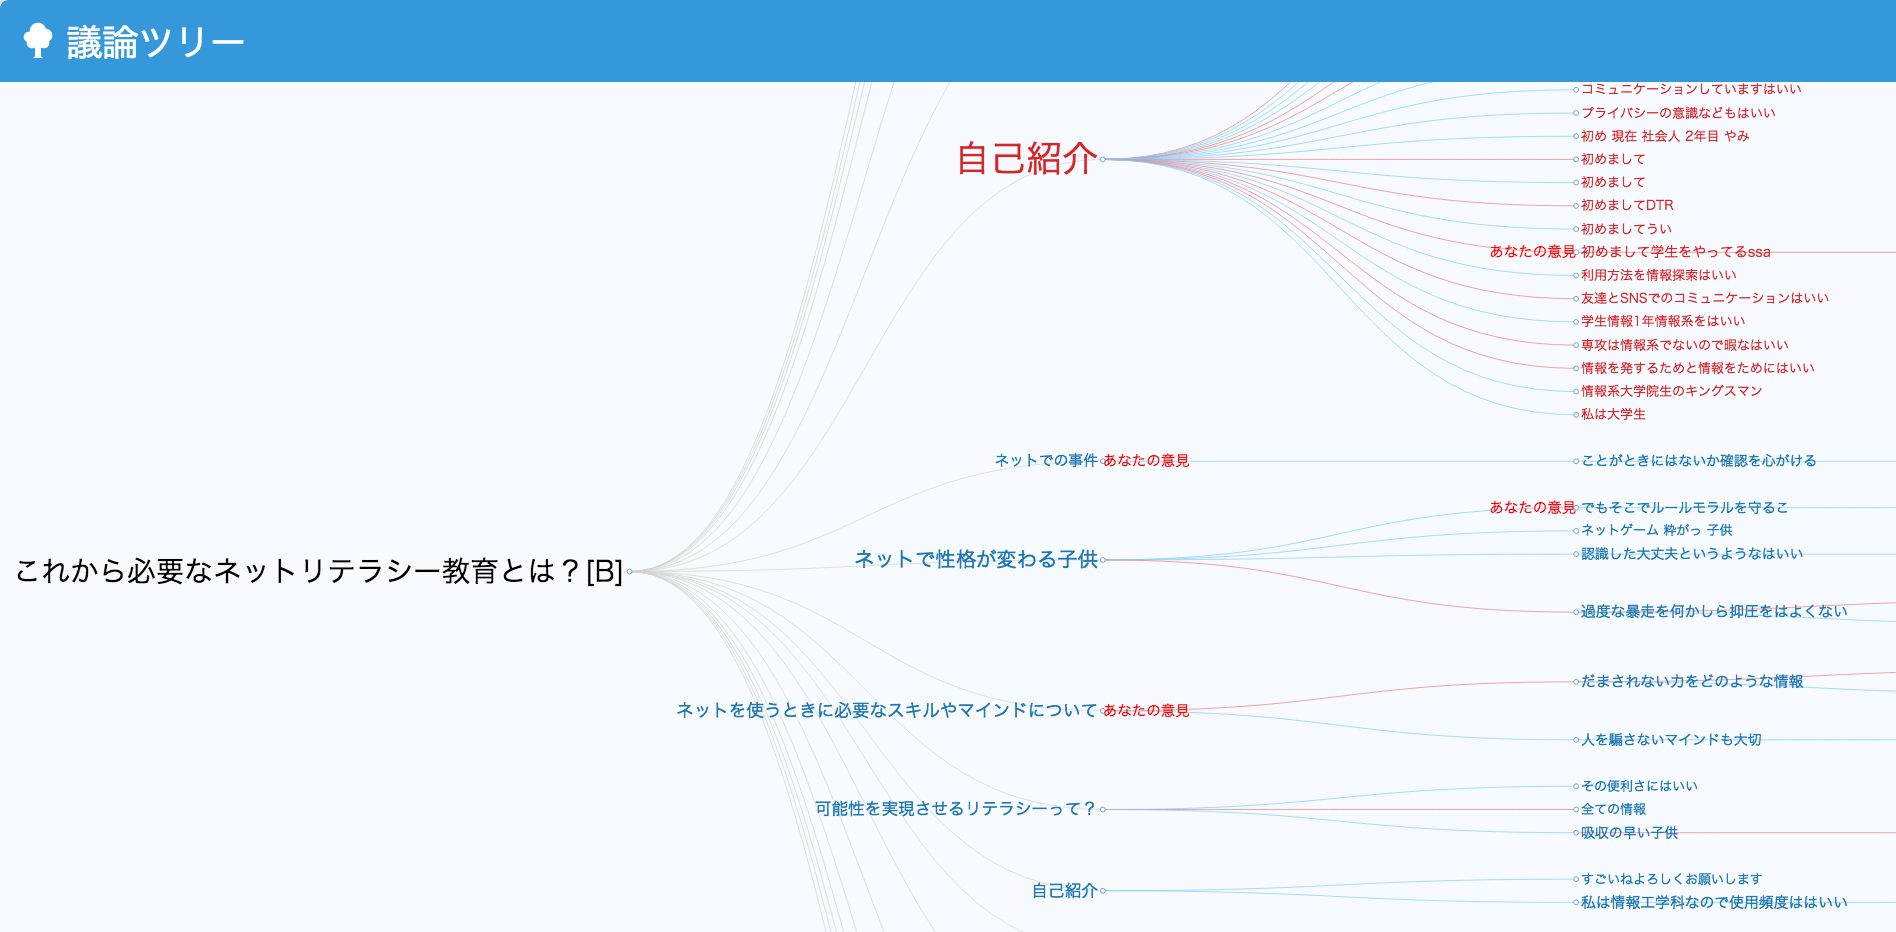
\includegraphics[width=\textwidth]{../images/2.Related_Work/argTree1.png}
  \caption{議論ツリー}
  \label{Fig:argTree1}
  \vspace{-10pt}
 \end{center}
\end{figure}
現行の機能では議論を見やすくすることに重点が置かれており,議論の把握の助けにはなるが画面に向き合う時間を減らすことにはなりにくい.むしろ,作業量を増やすことになり得ることもある.
従って,現行の支援機能ではファシリテーターの作業量の減少には繋がりにくい.
%
近年,自然言語処理の分野において分散表現が多くの研究で使われており,機械翻訳を始めとする単語の意味が重要となる分野で精度の向上が確認されている.分散表現を用いることで,人間に近い精度で話題の変化を観測することが可能となる.
%
以上のような背景を踏まえて,分散表現を用いて,話題の変化を観測し,話題の変化が確認された時にファシリテーターに伝えることが望ましい.
話題の変化の観測は,発言中に現れる単語の類似度の計算と見なすことができる.
分散表現を用いることで単語間の類似度を求めることができる,値が大きいほど単語がそれぞれ類似した実数ベクトルであることを表す.単語Aと単語Bの実数ベクトルが類似しているとは,単語Aと共に使われることの多い単語と単語Bと共に使われることの多い単語が多く共通していることを示す.故に,分散表現を使って単語の類似度を計算することができる.
%
発言文から単語を選ぶ際には自動要約を用いる.発言文から重要でない単語を取り除くことで関連度の計算の精度を高めることが可能となる.
要約の手法としてはokapi BM25 \cite{okapiBM25}とLexRankを組み合わせた抽出的要約手法を用いる.
\begin{comment}
%======================================= 社会的背景
2013年頃からWeb上での大規模な議論活動が活発になり,大規模な人数での議論が期待されている.
大規模な議論では意見を共有することは可能であるが,議論を整理させることや収束させることは難しい.以上から大規模意見集約システムCOLLAGREEが開発された.本システムではWeb上で適切に大規模な議論を行うことができるように議論をマネジメントするファシリテーターを導入した\cite{collagreeTest}.
過去の実験ではファシリテーターの存在が議論の集約に大きな役割を果たしていることが認識されており,大規模な議論のためにファシリテータは必要である.しかし,議論の規模に伴って議論時間が長くなる傾向があり,同時にファシリテーターは常に議論の動向を見続ける必要がある.故に,議論の規模が大きくなればなるほどファシリテーターは長時間かつ大規模な議論の動向の監視によって大きな負担がかかる.大規模な議論が増加する傾向を踏まえるとファシリテーターにかかる負担を軽減する支援が必要である.\\
以上の問題を解決するため,話題の変化を追い,重要な話題の転換点をファシリテーターの代わりに検出することが有用であると考える.必要な時にだけファシリテーターが画面を見れば良いようにすることでファシリテーターの負担軽減が期待できる.
%========================================= 現行手法問題点背景
%議論支援に関する先行研究において,既存の手法は全てが文字列を文字列のまま扱う手法である.
%既存手法は殆どがパターンマッチングと重み付けの2つに区分することができる.
%パターンマッチングでは事前に単語を登録して,単語がマッチした場合に処理を行うが,処理それぞれに対して単語を登録しなければならず手間が膨大になってしまう.また,単語の意味が考慮されておらず,手作業で登録を行うので登録漏れがあった場合に単語の意味に関係なく処理を行うことが不可能となってしまう.
%重み付けは単語の出現頻度や文章の長さを使用して単語・文章に順位を付ける手法で必ずしも単語の登録が必要でないため多くの研究で使用されている.
%しかし,重み付けもまた単語を文字列のまま扱っており,意味までは考慮されていない.故に ,人間なら対応できる似た単語でも1文字違うだけで対処が困難となる.
議論支援に関する先行研究においてファシリテーターに対する支援を目的としたものは無く,殆どが議論の活性化や可視化を目的としている.
%=================================新手法
近年,自然言語処理の分野において分散表現が多くの研究で使われており.分散表現は文字列である単語を辞書データを使用して実数ベクトルへと変換する.辞書データにない単語には対応できないが,多様な処理を1つの辞書データで行うことができる.また,実数ベクトルの各数値が単語の意味を表現するものとなっており,数値を使用して処理を行うことができる.
分散表現を用いることで既存手法より人間の感覚に近しい処理を行うことができる.
%=================================
以上のような背景を踏まえて,分散表現を用いてファシリテーターの代わりに話題の変化を判定し,知らせることを目指す.
話題転換の検出は発言同士の近さ,すなわち発言に含まれる単語意味の近さと見ることができる.
分散表現ではベクトル同士の内積計算を行うことで単語同士の意味の近さを計算することができる.
また,分散表現を使用することで機械翻訳を始めとする複数の分野で精度の向上が確認されている.
\end{comment}
\section{研究の目的}
\label{intro:taget}
本論文では,分散表現を用いて議論中での発言に含まれる単語の関連度を計算し,話題の変化を観測する手法を提案する.

\section{本論文の構成}
本論文の構成を以下に示す.
\ref{relwork:chapter} 章では要約手法に関する研究と,分散表現に関する先行研究を紹介する.
次に,\ref{model:chapter}章では発言の要約手法の説明を行い,\ref{impl:chapter}章では分散表現を用いた単語集合間の関連度計算について説明する.
そして,\ref{exp:chapter}章では話題転換点の検出の評価実験について説明する.
最後に\ref{con:chapter}章で本論文のまとめと考察を示す.

 %-------------------------------------------------------------------------------
 \expandafter\ifx\csname MasterFile\endcsname\relax
	\def\BibFile{hoge}
	\expandafter\ifx\csname MasterFile\endcsname\relax
\def\SubFile{hoge}
\documentclass[a4j,12pt,twoside,openany]{jreport}
%\nofiles %tocファイルを更新させない
%\documentclass[12pt,a4j,twoside,openany]{jsbook}
\usepackage[dvipdfmx]{graphicx}
\usepackage{../dspc} % ベースラインスキップの指定
\usepackage{../slashbox} % 表に斜線を入れる
%\usepackage{../mediabb}
\usepackage{fancyvrb} % Verbatim環境
\usepackage{fancyhdr} % Headerの下線付き章見出し
\usepackage{here} % float[H]
\usepackage{multirow}
\usepackage{hhline} % 表の罫線の角を美しくする
\usepackage{amsmath} %コレがないとcasesが動かない
\usepackage{amsfonts} % 数学用フォント
\usepackage{bm} % 数式環境での bold
\usepackage{algorithm}
\usepackage{algorithmicx}
\usepackage[noend]{algpseudocode}%\procedureはここに含まれる
\usepackage[flushleft]{threeparttable} % 脚注付きテーブル
\usepackage{enumitem}
\usepackage{comment}
\usepackage{fancybox}
%\usepackage{csvsimple,booktabs,siunitx}
%\usepackage{filecontents}
\usepackage{ulinej}


\setlength{\evensidemargin}{5pt}
\setlength{\oddsidemargin}{40pt}
%\setlength{\headheight}{16.5pt}
%%\setlength{\headheight}{30pt}
\setcounter{secnumdepth}{3}
\setlist[description]{leftmargin=2\parindent,labelindent=\parindent}

\makeatletter
\def\@makechapterhead#1{%
	\vspace*{50\p@}%
	{
		\parindent \z@ \raggedright \normalfont
		\ifnum \c@secnumdepth >\m@ne
		% \if@mainmatter
			\huge\bfseries\@chapapp\thechapter\@chappos
			\par\nobreak
			\vskip 20\p@
		% \fi
		\fi
		\interlinepenalty\@M
		\Huge\bfseries #1\par\nobreak
		\vskip 40\p@
	}
}

%新しいコマンド定義
\newcounter{linenumber}
\newenvironment{listing}{%
  \begin{list}{%
    \small\arabic{linenumber}:}{%
      \usecounter{linenumber}%
      \setlength{\baselineskip}{18pt}%
      \setlength{\itemsep}{0pt}%
      \setlength{\parsep}{0pt}}}%
 {\end{list}}
\newcommand{\figcaption}[1]{\def\@captype{figure}\caption{#1}}
\newcommand{\tblcaption}[1]{\def\@captype{table}\caption{#1}}
\newcommand{\norm}[1]{\left\| #1 \right\|}
\newcommand{\cc}[1]{\multicolumn{1}{|c|}{#1}}
\newcommand{\circled}[1]{\raisebox{.5pt}{\textcircled{\raisebox{-.9pt} {#1}}}}
\newcommand{\specialcell}[2][c]{%
  \begin{tabular}[#1]{@{}c@{}}#2\end{tabular}}
\makeatother
%===============================================================================
\expandafter\ifx\csname SubFile\endcsname\relax
\begin{document}
\def\MasterFile{hoge}
%-------------------------------------------------------------------------------
%\maketitle
\thispagestyle{empty}
\documentclass[a4j,12pt]{jarticle}
% 外表紙

% 題名
\def\title{降水量予測のための\\Sequence-to-Sequenceモデルに基づく\\マルチモーダル学習}
% 著者
\def\author{林 政行}
% 入学年度(平成)
\def\year{24}
% 学籍番号
\def\number{24115113}
% 指導教官
\def\kyoukan{伊藤孝行}
% 指導教官役職
\def\kyoukanrank{教授}
% 提出日
\def\teisyutubi{平成28年2月8日}

\begin{document}
\pagestyle{empty}
\baselineskip=18pt

\begin{center}

\vspace*{2cm}

{\huge \textbf{卒業論文}}

\vspace*{3cm}

%\vrule width 10cm height 1pt depth 0pt



%(題目)
%\vspace{5pt}
%\hrule height 3pt
%\vspace{1zh}

\vrule width 6.25cm height 6pt depth -2pt
\makebox[1.5cm]{(題目)}
\vrule width 6.25cm height 6pt depth -2pt

{\LARGE {\title}}

\vspace{1zh}
%{\large {\subtitle}}
%\hrule height 3pt
\vrule width 14cm height 4pt depth 0pt

\vspace*{1cm}

指導教員 {\large {\kyoukan}} {\kyoukanrank}

%\vspace*{5cm}
\vfill

{\large 名古屋工業大学 情報工学科}

{\large 平成{\year}年度 入学 ({\number})}

\vspace*{1cm}

%{\huge\mc {\author}}

\underline{(氏名)\hspace{3zw}{\huge\mc {\author}}\hspace{3zw}}

\vspace*{1cm}

({\teisyutubi}提出)

\vspace{2cm}
\end{center}

\end{document}
\begin{titlepage}

% 題名
\def\title{分散表現を用いた\\話題変化判定}
% 補助題名
\def\subtitle{卒業論文}
% 著者
\def\author{芳野 魁}
% 入学年度(平成)
\def\year{29}
% 学籍番号
\def\number{26115162}
% 指導教官
\def\kyoukan{伊藤 孝行}
% 指導教官役職
\def\kyoukanrank{教授}
% 提出日
\def\teisyutubi{平成29年9月19日}

\pagestyle{empty}

\begin{center}

\vspace*{20mm}
{\Large\mc 平成29年度 \hspace{7mm} 卒 業 論 文}
\vspace{15mm}

%\setlength{\unitlength}{1mm}
\begin{picture}(100,60)
  \put(0,0){\makebox(100,60){\huge\bf\shortstack{\title}}}
\end{picture}
\\
%\begin{picture}(100,5)
%  \put(0,0){\makebox(100,5){\Large\bf\shortstack{\subtitle}}}
%\end{picture}
\end{center}
\vspace{10mm}
\begin{flushright}
\begin{tabular}{ll}
{\large 提出日} & {\large {\teisyutubi}} \\
{\large 所属}  & {\large 名古屋工業大学 情報工学科} \\
{\large 指導教員} & {\large {\kyoukan} {\kyoukanrank}} \\
 & \\
{\large 入学年度} & {\large 平成{\year}年度入学}\\
{\large 学籍番号} &{\large {\number}} \\
 & \\
%{\large 氏名} & {\huge {\author}}
{\large 氏名} & {\huge\mc {\author}}
\end{tabular}
\end{flushright}

\end{titlepage}

%\addcontentsline{toc}{chapter}{表紙}
\thispagestyle{empty}
\mbox{}\newpage
%===============================================================================
%\frontmatter
%===============================================================================
%\mainmatter
%-------------------------------------------------------------------------------
\pagenumbering{arabic}
\cleardoublepage
\expandafter\ifx\csname MasterFile\endcsname\relax
\def\SubFile{hoge}
\input{../thesis/thesis}
\begin{document}
\fi
%-------------------------------------------------------------------------------
\cleardoublepage
\chapter*{論文要旨}\addcontentsline{toc}{chapter}{論文要旨}
近年,Web上での大規模な議論活動が活発になっているが,現在一般的に使われている "2ちゃんねる" や "Twitter" といったシステムでは整理や収束を行うことが困難である.困難である原因として,議論の管理を行う者がいないことが挙げられる.
議論を収束させるには議論のマネジメントを行う人物が必要である.
%
大規模意見集約システムCOLLAGREEではファシリテーターと呼ばれる人物が議論のマネジメントを行っている.
しかし,ファシリテーターは人間であり,長時間に渡って大人数での議論の動向をマネジメントし続けるのは困難である.
%
COLLAGREEで大規模な議論を収束させるためには,ファシリテーターが必要な時にだけ画面を見るようにして画面に向き合う時間を減らす工夫があることが望ましい.ファシリテーターが画面を見るべきタイミングは議論の話題が変化したときである.以前の議論の内容から外れた発言がされた時,ファシリテーターが適切に発言することで,脱線や炎上を避けて議論を収束させることができる.
すなわち,ファシリテーターの代わりに自動的に議論中の話題の変化を事前に判定することが求められている.
%
現在,COLLAGREE上で使用されている議論支援システムは投稿支援システムと議論可視化システムの2つに大別できる.
投稿支援システムはポイント機能やファシリテーションフレーズ簡易投稿機能のように,ユーザーが投稿をする際に何らかの補助やリアクションを行う.現行の機能では選択肢の提示に留まっており,作業量を減らすことには繋がりにくい。
一方,議論可視化システムは議論ツリーやキーワード抽出のように,ユーザーにスレッドとは異なる議論の見方を提供する.現行の機能では議論を見やすくすることに重点が置かれており,議論の把握の助けにはなるが画面に向き合う時間を減らすことにはなりにくい.むしろ,作業量を増やすことになり得る機能もある.
\begin{comment}
ポイント機能(ユーザの議論行動を活性化)-1
ファシリテーションフレーズ簡易投稿機能-1
議論ツリー-2
1文の要約,スレッドの要約,クラスタリング,返信意見の極性判定-2
ファシリテーションスタンプ-1
キーワード抽出-2
いいね機能-1
いいねランキング-2
投票機能-1
議論フェーズ機能-2
1-意見を出す、投稿をする際に補助や選択肢、リアクションを与える
2-議論の別の見方を提供する
\end{comment}
%
近年,自然言語処理の分野において分散表現が多くの研究で使われており,機械翻訳を始めとする単語の意味が重要となる分野で精度の向上が確認されている.分散表現を用いることで,人間に近い精度で話題の変化を観測することが可能となる.
%
以上のような背景を踏まえて,分散表現を用いて,話題の変化を観測し,話題の変化が確認された時にファシリテーターに伝えることが望ましい.
話題の変化の観測は,発言中に現れる単語の関連度合いの計算と見なすことができる.
分散表現を用いることで単語間の類似度を求めることができる,値が大きいほど単語がそれぞれ類似した実数ベクトルであることを表す.単語Aと単語Bの実数ベクトルが類似しているとは,単語Aと共に使われることの多い単語と単語Bと共に使われることの多い単語が多く共通していることを示す.故に,分散表現を使って単語の関連度を計算することができる.
%
発言文から単語を選ぶ際には自動要約を用いる.発言文から重要でない単語を取り除くことで関連度の計算の精度を高めることが可能となる.
%
本論文では,分散表現を用いて議論中での発言に含まれる単語の関連度を計算し,話題の変化を観測する手法を提案する.
%
提案手法は,既存の抽出的要約手法を用いて選ばれた単語の関連度を計算する手法,Seq2Seqによる生成的要約を用いて生成された単語の関連度を計算する手法,オントロジーを用いて求められた単語の関連度を計算する手法の3つである.
提案した3つの手法により,議論中の話題の変化の観測の評価実験を行い,各手法の評価を行う.
評価実験によって,提案手法を用いることで人間の代わりに自動的に話題の変化を観測できることを確認する.
%
 \begin{comment}
大規模な議論では意見を共有することは可能であるが,議論を整理させることや収束させることは難しい.以上から大規模意見集約システムCOLLAGREEが開発された.本システムではWeb上で適切に大規模な議論を行うことができるように議論をマネジメントするファシリテーターを導入した.
過去の実験ではファシリテーターの存在が議論の集約に大きな役割を果たしていることが認識されており,大規模な議論のためにファシリテータは必要である.しかし,議論の規模に伴って議論時間が長くなる傾向があり,同時にファシリテーターは常に議論の動向を見続ける必要がある.故に,議論の規模が大きくなればなるほどファシリテーターは長時間かつ大規模な議論の動向の監視によって大きな負担がかかる.大規模な議論が増加する傾向を踏まえるとファシリテーターにかかる負担を軽減する支援が必要となることは明白である.
また,近年自然言語処理の分野において分散表現が多くの研究で使われており,機械翻訳を始めとする複数の分野で精度の向上が確認されている.まだ適応されていない分野でも結果の向上が期待できる.
従って,本研究では負担軽減の1つとして分散表現を用いて議論中での話題の変化を人間の代わりに検知することでファシリテーターの負担を軽減することを目指す.
-----------------

\end{comment}
%-------------------------------------------------------------------------------
\expandafter\ifx\csname MasterFile\endcsname\relax
\end{document}
\fi

%-------------------------------------------------------------------------------
\clearpage
\addcontentsline{toc}{chapter}{目次}
\tableofcontents

\clearpage
\addcontentsline{toc}{chapter}{図目次}
\listoffigures

\clearpage
\addcontentsline{toc}{chapter}{表目次}
\listoftables

%-------------------------------------------------------------------------------

%=====================
\pagestyle{fancy} % Headerをつける
\renewcommand{\sectionmark}[1]{\markright{\thesection\ \ \ #1}}
\renewcommand{\chaptermark}[1]{\markboth{#1}{}}
\lhead{}
\chead{}
\lfoot{}
\rfoot{}%-------------------------------------------------------------------------------
\expandafter\ifx\csname MasterFile\endcsname\relax
\def\SubFile{hoge}
\input{../thesis/thesis}
\begin{document}
\fi
%-------------------------------------------------------------------------------
\cleardoublepage
\chapter*{論文要旨}\addcontentsline{toc}{chapter}{論文要旨}
近年,Web上での大規模な議論活動が活発になっているが,現在一般的に使われている "2ちゃんねる" や "Twitter" といったシステムでは整理や収束を行うことが困難である.困難である原因として,議論の管理を行う者がいないことが挙げられる.
議論を収束させるには議論のマネジメントを行う人物が必要である.
%
大規模意見集約システムCOLLAGREEではファシリテーターと呼ばれる人物が議論のマネジメントを行っている.
しかし,ファシリテーターは人間であり,長時間に渡って大人数での議論の動向をマネジメントし続けるのは困難である.
%
COLLAGREEで大規模な議論を収束させるためには,ファシリテーターが必要な時にだけ画面を見るようにして画面に向き合う時間を減らす工夫があることが望ましい.ファシリテーターが画面を見るべきタイミングは議論の話題が変化したときである.以前の議論の内容から外れた発言がされた時,ファシリテーターが適切に発言することで,脱線や炎上を避けて議論を収束させることができる.
すなわち,ファシリテーターの代わりに自動的に議論中の話題の変化を事前に判定することが求められている.
%
現在,COLLAGREE上で使用されている議論支援システムは投稿支援システムと議論可視化システムの2つに大別できる.
投稿支援システムはポイント機能やファシリテーションフレーズ簡易投稿機能のように,ユーザーが投稿をする際に何らかの補助やリアクションを行う.現行の機能では選択肢の提示に留まっており,作業量を減らすことには繋がりにくい。
一方,議論可視化システムは議論ツリーやキーワード抽出のように,ユーザーにスレッドとは異なる議論の見方を提供する.現行の機能では議論を見やすくすることに重点が置かれており,議論の把握の助けにはなるが画面に向き合う時間を減らすことにはなりにくい.むしろ,作業量を増やすことになり得る機能もある.
\begin{comment}
ポイント機能(ユーザの議論行動を活性化)-1
ファシリテーションフレーズ簡易投稿機能-1
議論ツリー-2
1文の要約,スレッドの要約,クラスタリング,返信意見の極性判定-2
ファシリテーションスタンプ-1
キーワード抽出-2
いいね機能-1
いいねランキング-2
投票機能-1
議論フェーズ機能-2
1-意見を出す、投稿をする際に補助や選択肢、リアクションを与える
2-議論の別の見方を提供する
\end{comment}
%
近年,自然言語処理の分野において分散表現が多くの研究で使われており,機械翻訳を始めとする単語の意味が重要となる分野で精度の向上が確認されている.分散表現を用いることで,人間に近い精度で話題の変化を観測することが可能となる.
%
以上のような背景を踏まえて,分散表現を用いて,話題の変化を観測し,話題の変化が確認された時にファシリテーターに伝えることが望ましい.
話題の変化の観測は,発言中に現れる単語の関連度合いの計算と見なすことができる.
分散表現を用いることで単語間の類似度を求めることができる,値が大きいほど単語がそれぞれ類似した実数ベクトルであることを表す.単語Aと単語Bの実数ベクトルが類似しているとは,単語Aと共に使われることの多い単語と単語Bと共に使われることの多い単語が多く共通していることを示す.故に,分散表現を使って単語の関連度を計算することができる.
%
発言文から単語を選ぶ際には自動要約を用いる.発言文から重要でない単語を取り除くことで関連度の計算の精度を高めることが可能となる.
%
本論文では,分散表現を用いて議論中での発言に含まれる単語の関連度を計算し,話題の変化を観測する手法を提案する.
%
提案手法は,既存の抽出的要約手法を用いて選ばれた単語の関連度を計算する手法,Seq2Seqによる生成的要約を用いて生成された単語の関連度を計算する手法,オントロジーを用いて求められた単語の関連度を計算する手法の3つである.
提案した3つの手法により,議論中の話題の変化の観測の評価実験を行い,各手法の評価を行う.
評価実験によって,提案手法を用いることで人間の代わりに自動的に話題の変化を観測できることを確認する.
%
 \begin{comment}
大規模な議論では意見を共有することは可能であるが,議論を整理させることや収束させることは難しい.以上から大規模意見集約システムCOLLAGREEが開発された.本システムではWeb上で適切に大規模な議論を行うことができるように議論をマネジメントするファシリテーターを導入した.
過去の実験ではファシリテーターの存在が議論の集約に大きな役割を果たしていることが認識されており,大規模な議論のためにファシリテータは必要である.しかし,議論の規模に伴って議論時間が長くなる傾向があり,同時にファシリテーターは常に議論の動向を見続ける必要がある.故に,議論の規模が大きくなればなるほどファシリテーターは長時間かつ大規模な議論の動向の監視によって大きな負担がかかる.大規模な議論が増加する傾向を踏まえるとファシリテーターにかかる負担を軽減する支援が必要となることは明白である.
また,近年自然言語処理の分野において分散表現が多くの研究で使われており,機械翻訳を始めとする複数の分野で精度の向上が確認されている.まだ適応されていない分野でも結果の向上が期待できる.
従って,本研究では負担軽減の1つとして分散表現を用いて議論中での話題の変化を人間の代わりに検知することでファシリテーターの負担を軽減することを目指す.
-----------------

\end{comment}
%-------------------------------------------------------------------------------
\expandafter\ifx\csname MasterFile\endcsname\relax
\end{document}
\fi

%-------------------------------------------------------------------------------
\expandafter\ifx\csname MasterFile\endcsname\relax
\def\SubFile{hoge}
\input{../thesis/thesis}
\begin{document}
\fi
%-------------------------------------------------------------------------------
\cleardoublepage
\chapter*{論文要旨}\addcontentsline{toc}{chapter}{論文要旨}
近年,Web上での大規模な議論活動が活発になっているが,現在一般的に使われている "2ちゃんねる" や "Twitter" といったシステムでは整理や収束を行うことが困難である.困難である原因として,議論の管理を行う者がいないことが挙げられる.
議論を収束させるには議論のマネジメントを行う人物が必要である.
%
大規模意見集約システムCOLLAGREEではファシリテーターと呼ばれる人物が議論のマネジメントを行っている.
しかし,ファシリテーターは人間であり,長時間に渡って大人数での議論の動向をマネジメントし続けるのは困難である.
%
COLLAGREEで大規模な議論を収束させるためには,ファシリテーターが必要な時にだけ画面を見るようにして画面に向き合う時間を減らす工夫があることが望ましい.ファシリテーターが画面を見るべきタイミングは議論の話題が変化したときである.以前の議論の内容から外れた発言がされた時,ファシリテーターが適切に発言することで,脱線や炎上を避けて議論を収束させることができる.
すなわち,ファシリテーターの代わりに自動的に議論中の話題の変化を事前に判定することが求められている.
%
現在,COLLAGREE上で使用されている議論支援システムは投稿支援システムと議論可視化システムの2つに大別できる.
投稿支援システムはポイント機能やファシリテーションフレーズ簡易投稿機能のように,ユーザーが投稿をする際に何らかの補助やリアクションを行う.現行の機能では選択肢の提示に留まっており,作業量を減らすことには繋がりにくい。
一方,議論可視化システムは議論ツリーやキーワード抽出のように,ユーザーにスレッドとは異なる議論の見方を提供する.現行の機能では議論を見やすくすることに重点が置かれており,議論の把握の助けにはなるが画面に向き合う時間を減らすことにはなりにくい.むしろ,作業量を増やすことになり得る機能もある.
\begin{comment}
ポイント機能(ユーザの議論行動を活性化)-1
ファシリテーションフレーズ簡易投稿機能-1
議論ツリー-2
1文の要約,スレッドの要約,クラスタリング,返信意見の極性判定-2
ファシリテーションスタンプ-1
キーワード抽出-2
いいね機能-1
いいねランキング-2
投票機能-1
議論フェーズ機能-2
1-意見を出す、投稿をする際に補助や選択肢、リアクションを与える
2-議論の別の見方を提供する
\end{comment}
%
近年,自然言語処理の分野において分散表現が多くの研究で使われており,機械翻訳を始めとする単語の意味が重要となる分野で精度の向上が確認されている.分散表現を用いることで,人間に近い精度で話題の変化を観測することが可能となる.
%
以上のような背景を踏まえて,分散表現を用いて,話題の変化を観測し,話題の変化が確認された時にファシリテーターに伝えることが望ましい.
話題の変化の観測は,発言中に現れる単語の関連度合いの計算と見なすことができる.
分散表現を用いることで単語間の類似度を求めることができる,値が大きいほど単語がそれぞれ類似した実数ベクトルであることを表す.単語Aと単語Bの実数ベクトルが類似しているとは,単語Aと共に使われることの多い単語と単語Bと共に使われることの多い単語が多く共通していることを示す.故に,分散表現を使って単語の関連度を計算することができる.
%
発言文から単語を選ぶ際には自動要約を用いる.発言文から重要でない単語を取り除くことで関連度の計算の精度を高めることが可能となる.
%
本論文では,分散表現を用いて議論中での発言に含まれる単語の関連度を計算し,話題の変化を観測する手法を提案する.
%
提案手法は,既存の抽出的要約手法を用いて選ばれた単語の関連度を計算する手法,Seq2Seqによる生成的要約を用いて生成された単語の関連度を計算する手法,オントロジーを用いて求められた単語の関連度を計算する手法の3つである.
提案した3つの手法により,議論中の話題の変化の観測の評価実験を行い,各手法の評価を行う.
評価実験によって,提案手法を用いることで人間の代わりに自動的に話題の変化を観測できることを確認する.
%
 \begin{comment}
大規模な議論では意見を共有することは可能であるが,議論を整理させることや収束させることは難しい.以上から大規模意見集約システムCOLLAGREEが開発された.本システムではWeb上で適切に大規模な議論を行うことができるように議論をマネジメントするファシリテーターを導入した.
過去の実験ではファシリテーターの存在が議論の集約に大きな役割を果たしていることが認識されており,大規模な議論のためにファシリテータは必要である.しかし,議論の規模に伴って議論時間が長くなる傾向があり,同時にファシリテーターは常に議論の動向を見続ける必要がある.故に,議論の規模が大きくなればなるほどファシリテーターは長時間かつ大規模な議論の動向の監視によって大きな負担がかかる.大規模な議論が増加する傾向を踏まえるとファシリテーターにかかる負担を軽減する支援が必要となることは明白である.
また,近年自然言語処理の分野において分散表現が多くの研究で使われており,機械翻訳を始めとする複数の分野で精度の向上が確認されている.まだ適応されていない分野でも結果の向上が期待できる.
従って,本研究では負担軽減の1つとして分散表現を用いて議論中での話題の変化を人間の代わりに検知することでファシリテーターの負担を軽減することを目指す.
-----------------

\end{comment}
%-------------------------------------------------------------------------------
\expandafter\ifx\csname MasterFile\endcsname\relax
\end{document}
\fi

%-------------------------------------------------------------------------------
\expandafter\ifx\csname MasterFile\endcsname\relax
\def\SubFile{hoge}
\input{../thesis/thesis}
\begin{document}
\fi
%-------------------------------------------------------------------------------
\cleardoublepage
\chapter*{論文要旨}\addcontentsline{toc}{chapter}{論文要旨}
近年,Web上での大規模な議論活動が活発になっているが,現在一般的に使われている "2ちゃんねる" や "Twitter" といったシステムでは整理や収束を行うことが困難である.困難である原因として,議論の管理を行う者がいないことが挙げられる.
議論を収束させるには議論のマネジメントを行う人物が必要である.
%
大規模意見集約システムCOLLAGREEではファシリテーターと呼ばれる人物が議論のマネジメントを行っている.
しかし,ファシリテーターは人間であり,長時間に渡って大人数での議論の動向をマネジメントし続けるのは困難である.
%
COLLAGREEで大規模な議論を収束させるためには,ファシリテーターが必要な時にだけ画面を見るようにして画面に向き合う時間を減らす工夫があることが望ましい.ファシリテーターが画面を見るべきタイミングは議論の話題が変化したときである.以前の議論の内容から外れた発言がされた時,ファシリテーターが適切に発言することで,脱線や炎上を避けて議論を収束させることができる.
すなわち,ファシリテーターの代わりに自動的に議論中の話題の変化を事前に判定することが求められている.
%
現在,COLLAGREE上で使用されている議論支援システムは投稿支援システムと議論可視化システムの2つに大別できる.
投稿支援システムはポイント機能やファシリテーションフレーズ簡易投稿機能のように,ユーザーが投稿をする際に何らかの補助やリアクションを行う.現行の機能では選択肢の提示に留まっており,作業量を減らすことには繋がりにくい。
一方,議論可視化システムは議論ツリーやキーワード抽出のように,ユーザーにスレッドとは異なる議論の見方を提供する.現行の機能では議論を見やすくすることに重点が置かれており,議論の把握の助けにはなるが画面に向き合う時間を減らすことにはなりにくい.むしろ,作業量を増やすことになり得る機能もある.
\begin{comment}
ポイント機能(ユーザの議論行動を活性化)-1
ファシリテーションフレーズ簡易投稿機能-1
議論ツリー-2
1文の要約,スレッドの要約,クラスタリング,返信意見の極性判定-2
ファシリテーションスタンプ-1
キーワード抽出-2
いいね機能-1
いいねランキング-2
投票機能-1
議論フェーズ機能-2
1-意見を出す、投稿をする際に補助や選択肢、リアクションを与える
2-議論の別の見方を提供する
\end{comment}
%
近年,自然言語処理の分野において分散表現が多くの研究で使われており,機械翻訳を始めとする単語の意味が重要となる分野で精度の向上が確認されている.分散表現を用いることで,人間に近い精度で話題の変化を観測することが可能となる.
%
以上のような背景を踏まえて,分散表現を用いて,話題の変化を観測し,話題の変化が確認された時にファシリテーターに伝えることが望ましい.
話題の変化の観測は,発言中に現れる単語の関連度合いの計算と見なすことができる.
分散表現を用いることで単語間の類似度を求めることができる,値が大きいほど単語がそれぞれ類似した実数ベクトルであることを表す.単語Aと単語Bの実数ベクトルが類似しているとは,単語Aと共に使われることの多い単語と単語Bと共に使われることの多い単語が多く共通していることを示す.故に,分散表現を使って単語の関連度を計算することができる.
%
発言文から単語を選ぶ際には自動要約を用いる.発言文から重要でない単語を取り除くことで関連度の計算の精度を高めることが可能となる.
%
本論文では,分散表現を用いて議論中での発言に含まれる単語の関連度を計算し,話題の変化を観測する手法を提案する.
%
提案手法は,既存の抽出的要約手法を用いて選ばれた単語の関連度を計算する手法,Seq2Seqによる生成的要約を用いて生成された単語の関連度を計算する手法,オントロジーを用いて求められた単語の関連度を計算する手法の3つである.
提案した3つの手法により,議論中の話題の変化の観測の評価実験を行い,各手法の評価を行う.
評価実験によって,提案手法を用いることで人間の代わりに自動的に話題の変化を観測できることを確認する.
%
 \begin{comment}
大規模な議論では意見を共有することは可能であるが,議論を整理させることや収束させることは難しい.以上から大規模意見集約システムCOLLAGREEが開発された.本システムではWeb上で適切に大規模な議論を行うことができるように議論をマネジメントするファシリテーターを導入した.
過去の実験ではファシリテーターの存在が議論の集約に大きな役割を果たしていることが認識されており,大規模な議論のためにファシリテータは必要である.しかし,議論の規模に伴って議論時間が長くなる傾向があり,同時にファシリテーターは常に議論の動向を見続ける必要がある.故に,議論の規模が大きくなればなるほどファシリテーターは長時間かつ大規模な議論の動向の監視によって大きな負担がかかる.大規模な議論が増加する傾向を踏まえるとファシリテーターにかかる負担を軽減する支援が必要となることは明白である.
また,近年自然言語処理の分野において分散表現が多くの研究で使われており,機械翻訳を始めとする複数の分野で精度の向上が確認されている.まだ適応されていない分野でも結果の向上が期待できる.
従って,本研究では負担軽減の1つとして分散表現を用いて議論中での話題の変化を人間の代わりに検知することでファシリテーターの負担を軽減することを目指す.
-----------------

\end{comment}
%-------------------------------------------------------------------------------
\expandafter\ifx\csname MasterFile\endcsname\relax
\end{document}
\fi

%-------------------------------------------------------------------------------
\expandafter\ifx\csname MasterFile\endcsname\relax
\def\SubFile{hoge}
\input{../thesis/thesis}
\begin{document}
\fi
%-------------------------------------------------------------------------------
\cleardoublepage
\chapter*{論文要旨}\addcontentsline{toc}{chapter}{論文要旨}
近年,Web上での大規模な議論活動が活発になっているが,現在一般的に使われている "2ちゃんねる" や "Twitter" といったシステムでは整理や収束を行うことが困難である.困難である原因として,議論の管理を行う者がいないことが挙げられる.
議論を収束させるには議論のマネジメントを行う人物が必要である.
%
大規模意見集約システムCOLLAGREEではファシリテーターと呼ばれる人物が議論のマネジメントを行っている.
しかし,ファシリテーターは人間であり,長時間に渡って大人数での議論の動向をマネジメントし続けるのは困難である.
%
COLLAGREEで大規模な議論を収束させるためには,ファシリテーターが必要な時にだけ画面を見るようにして画面に向き合う時間を減らす工夫があることが望ましい.ファシリテーターが画面を見るべきタイミングは議論の話題が変化したときである.以前の議論の内容から外れた発言がされた時,ファシリテーターが適切に発言することで,脱線や炎上を避けて議論を収束させることができる.
すなわち,ファシリテーターの代わりに自動的に議論中の話題の変化を事前に判定することが求められている.
%
現在,COLLAGREE上で使用されている議論支援システムは投稿支援システムと議論可視化システムの2つに大別できる.
投稿支援システムはポイント機能やファシリテーションフレーズ簡易投稿機能のように,ユーザーが投稿をする際に何らかの補助やリアクションを行う.現行の機能では選択肢の提示に留まっており,作業量を減らすことには繋がりにくい。
一方,議論可視化システムは議論ツリーやキーワード抽出のように,ユーザーにスレッドとは異なる議論の見方を提供する.現行の機能では議論を見やすくすることに重点が置かれており,議論の把握の助けにはなるが画面に向き合う時間を減らすことにはなりにくい.むしろ,作業量を増やすことになり得る機能もある.
\begin{comment}
ポイント機能(ユーザの議論行動を活性化)-1
ファシリテーションフレーズ簡易投稿機能-1
議論ツリー-2
1文の要約,スレッドの要約,クラスタリング,返信意見の極性判定-2
ファシリテーションスタンプ-1
キーワード抽出-2
いいね機能-1
いいねランキング-2
投票機能-1
議論フェーズ機能-2
1-意見を出す、投稿をする際に補助や選択肢、リアクションを与える
2-議論の別の見方を提供する
\end{comment}
%
近年,自然言語処理の分野において分散表現が多くの研究で使われており,機械翻訳を始めとする単語の意味が重要となる分野で精度の向上が確認されている.分散表現を用いることで,人間に近い精度で話題の変化を観測することが可能となる.
%
以上のような背景を踏まえて,分散表現を用いて,話題の変化を観測し,話題の変化が確認された時にファシリテーターに伝えることが望ましい.
話題の変化の観測は,発言中に現れる単語の関連度合いの計算と見なすことができる.
分散表現を用いることで単語間の類似度を求めることができる,値が大きいほど単語がそれぞれ類似した実数ベクトルであることを表す.単語Aと単語Bの実数ベクトルが類似しているとは,単語Aと共に使われることの多い単語と単語Bと共に使われることの多い単語が多く共通していることを示す.故に,分散表現を使って単語の関連度を計算することができる.
%
発言文から単語を選ぶ際には自動要約を用いる.発言文から重要でない単語を取り除くことで関連度の計算の精度を高めることが可能となる.
%
本論文では,分散表現を用いて議論中での発言に含まれる単語の関連度を計算し,話題の変化を観測する手法を提案する.
%
提案手法は,既存の抽出的要約手法を用いて選ばれた単語の関連度を計算する手法,Seq2Seqによる生成的要約を用いて生成された単語の関連度を計算する手法,オントロジーを用いて求められた単語の関連度を計算する手法の3つである.
提案した3つの手法により,議論中の話題の変化の観測の評価実験を行い,各手法の評価を行う.
評価実験によって,提案手法を用いることで人間の代わりに自動的に話題の変化を観測できることを確認する.
%
 \begin{comment}
大規模な議論では意見を共有することは可能であるが,議論を整理させることや収束させることは難しい.以上から大規模意見集約システムCOLLAGREEが開発された.本システムではWeb上で適切に大規模な議論を行うことができるように議論をマネジメントするファシリテーターを導入した.
過去の実験ではファシリテーターの存在が議論の集約に大きな役割を果たしていることが認識されており,大規模な議論のためにファシリテータは必要である.しかし,議論の規模に伴って議論時間が長くなる傾向があり,同時にファシリテーターは常に議論の動向を見続ける必要がある.故に,議論の規模が大きくなればなるほどファシリテーターは長時間かつ大規模な議論の動向の監視によって大きな負担がかかる.大規模な議論が増加する傾向を踏まえるとファシリテーターにかかる負担を軽減する支援が必要となることは明白である.
また,近年自然言語処理の分野において分散表現が多くの研究で使われており,機械翻訳を始めとする複数の分野で精度の向上が確認されている.まだ適応されていない分野でも結果の向上が期待できる.
従って,本研究では負担軽減の1つとして分散表現を用いて議論中での話題の変化を人間の代わりに検知することでファシリテーターの負担を軽減することを目指す.
-----------------

\end{comment}
%-------------------------------------------------------------------------------
\expandafter\ifx\csname MasterFile\endcsname\relax
\end{document}
\fi

%-------------------------------------------------------------------------------
\expandafter\ifx\csname MasterFile\endcsname\relax
\def\SubFile{hoge}
\input{../thesis/thesis}
\begin{document}
\fi
%-------------------------------------------------------------------------------
\cleardoublepage
\chapter*{論文要旨}\addcontentsline{toc}{chapter}{論文要旨}
近年,Web上での大規模な議論活動が活発になっているが,現在一般的に使われている "2ちゃんねる" や "Twitter" といったシステムでは整理や収束を行うことが困難である.困難である原因として,議論の管理を行う者がいないことが挙げられる.
議論を収束させるには議論のマネジメントを行う人物が必要である.
%
大規模意見集約システムCOLLAGREEではファシリテーターと呼ばれる人物が議論のマネジメントを行っている.
しかし,ファシリテーターは人間であり,長時間に渡って大人数での議論の動向をマネジメントし続けるのは困難である.
%
COLLAGREEで大規模な議論を収束させるためには,ファシリテーターが必要な時にだけ画面を見るようにして画面に向き合う時間を減らす工夫があることが望ましい.ファシリテーターが画面を見るべきタイミングは議論の話題が変化したときである.以前の議論の内容から外れた発言がされた時,ファシリテーターが適切に発言することで,脱線や炎上を避けて議論を収束させることができる.
すなわち,ファシリテーターの代わりに自動的に議論中の話題の変化を事前に判定することが求められている.
%
現在,COLLAGREE上で使用されている議論支援システムは投稿支援システムと議論可視化システムの2つに大別できる.
投稿支援システムはポイント機能やファシリテーションフレーズ簡易投稿機能のように,ユーザーが投稿をする際に何らかの補助やリアクションを行う.現行の機能では選択肢の提示に留まっており,作業量を減らすことには繋がりにくい。
一方,議論可視化システムは議論ツリーやキーワード抽出のように,ユーザーにスレッドとは異なる議論の見方を提供する.現行の機能では議論を見やすくすることに重点が置かれており,議論の把握の助けにはなるが画面に向き合う時間を減らすことにはなりにくい.むしろ,作業量を増やすことになり得る機能もある.
\begin{comment}
ポイント機能(ユーザの議論行動を活性化)-1
ファシリテーションフレーズ簡易投稿機能-1
議論ツリー-2
1文の要約,スレッドの要約,クラスタリング,返信意見の極性判定-2
ファシリテーションスタンプ-1
キーワード抽出-2
いいね機能-1
いいねランキング-2
投票機能-1
議論フェーズ機能-2
1-意見を出す、投稿をする際に補助や選択肢、リアクションを与える
2-議論の別の見方を提供する
\end{comment}
%
近年,自然言語処理の分野において分散表現が多くの研究で使われており,機械翻訳を始めとする単語の意味が重要となる分野で精度の向上が確認されている.分散表現を用いることで,人間に近い精度で話題の変化を観測することが可能となる.
%
以上のような背景を踏まえて,分散表現を用いて,話題の変化を観測し,話題の変化が確認された時にファシリテーターに伝えることが望ましい.
話題の変化の観測は,発言中に現れる単語の関連度合いの計算と見なすことができる.
分散表現を用いることで単語間の類似度を求めることができる,値が大きいほど単語がそれぞれ類似した実数ベクトルであることを表す.単語Aと単語Bの実数ベクトルが類似しているとは,単語Aと共に使われることの多い単語と単語Bと共に使われることの多い単語が多く共通していることを示す.故に,分散表現を使って単語の関連度を計算することができる.
%
発言文から単語を選ぶ際には自動要約を用いる.発言文から重要でない単語を取り除くことで関連度の計算の精度を高めることが可能となる.
%
本論文では,分散表現を用いて議論中での発言に含まれる単語の関連度を計算し,話題の変化を観測する手法を提案する.
%
提案手法は,既存の抽出的要約手法を用いて選ばれた単語の関連度を計算する手法,Seq2Seqによる生成的要約を用いて生成された単語の関連度を計算する手法,オントロジーを用いて求められた単語の関連度を計算する手法の3つである.
提案した3つの手法により,議論中の話題の変化の観測の評価実験を行い,各手法の評価を行う.
評価実験によって,提案手法を用いることで人間の代わりに自動的に話題の変化を観測できることを確認する.
%
 \begin{comment}
大規模な議論では意見を共有することは可能であるが,議論を整理させることや収束させることは難しい.以上から大規模意見集約システムCOLLAGREEが開発された.本システムではWeb上で適切に大規模な議論を行うことができるように議論をマネジメントするファシリテーターを導入した.
過去の実験ではファシリテーターの存在が議論の集約に大きな役割を果たしていることが認識されており,大規模な議論のためにファシリテータは必要である.しかし,議論の規模に伴って議論時間が長くなる傾向があり,同時にファシリテーターは常に議論の動向を見続ける必要がある.故に,議論の規模が大きくなればなるほどファシリテーターは長時間かつ大規模な議論の動向の監視によって大きな負担がかかる.大規模な議論が増加する傾向を踏まえるとファシリテーターにかかる負担を軽減する支援が必要となることは明白である.
また,近年自然言語処理の分野において分散表現が多くの研究で使われており,機械翻訳を始めとする複数の分野で精度の向上が確認されている.まだ適応されていない分野でも結果の向上が期待できる.
従って,本研究では負担軽減の1つとして分散表現を用いて議論中での話題の変化を人間の代わりに検知することでファシリテーターの負担を軽減することを目指す.
-----------------

\end{comment}
%-------------------------------------------------------------------------------
\expandafter\ifx\csname MasterFile\endcsname\relax
\end{document}
\fi

%-------------------------------------------------------------------------------
\expandafter\ifx\csname MasterFile\endcsname\relax
\def\SubFile{hoge}
\input{../thesis/thesis}
\begin{document}
\fi
%-------------------------------------------------------------------------------
\cleardoublepage
\chapter*{論文要旨}\addcontentsline{toc}{chapter}{論文要旨}
近年,Web上での大規模な議論活動が活発になっているが,現在一般的に使われている "2ちゃんねる" や "Twitter" といったシステムでは整理や収束を行うことが困難である.困難である原因として,議論の管理を行う者がいないことが挙げられる.
議論を収束させるには議論のマネジメントを行う人物が必要である.
%
大規模意見集約システムCOLLAGREEではファシリテーターと呼ばれる人物が議論のマネジメントを行っている.
しかし,ファシリテーターは人間であり,長時間に渡って大人数での議論の動向をマネジメントし続けるのは困難である.
%
COLLAGREEで大規模な議論を収束させるためには,ファシリテーターが必要な時にだけ画面を見るようにして画面に向き合う時間を減らす工夫があることが望ましい.ファシリテーターが画面を見るべきタイミングは議論の話題が変化したときである.以前の議論の内容から外れた発言がされた時,ファシリテーターが適切に発言することで,脱線や炎上を避けて議論を収束させることができる.
すなわち,ファシリテーターの代わりに自動的に議論中の話題の変化を事前に判定することが求められている.
%
現在,COLLAGREE上で使用されている議論支援システムは投稿支援システムと議論可視化システムの2つに大別できる.
投稿支援システムはポイント機能やファシリテーションフレーズ簡易投稿機能のように,ユーザーが投稿をする際に何らかの補助やリアクションを行う.現行の機能では選択肢の提示に留まっており,作業量を減らすことには繋がりにくい。
一方,議論可視化システムは議論ツリーやキーワード抽出のように,ユーザーにスレッドとは異なる議論の見方を提供する.現行の機能では議論を見やすくすることに重点が置かれており,議論の把握の助けにはなるが画面に向き合う時間を減らすことにはなりにくい.むしろ,作業量を増やすことになり得る機能もある.
\begin{comment}
ポイント機能(ユーザの議論行動を活性化)-1
ファシリテーションフレーズ簡易投稿機能-1
議論ツリー-2
1文の要約,スレッドの要約,クラスタリング,返信意見の極性判定-2
ファシリテーションスタンプ-1
キーワード抽出-2
いいね機能-1
いいねランキング-2
投票機能-1
議論フェーズ機能-2
1-意見を出す、投稿をする際に補助や選択肢、リアクションを与える
2-議論の別の見方を提供する
\end{comment}
%
近年,自然言語処理の分野において分散表現が多くの研究で使われており,機械翻訳を始めとする単語の意味が重要となる分野で精度の向上が確認されている.分散表現を用いることで,人間に近い精度で話題の変化を観測することが可能となる.
%
以上のような背景を踏まえて,分散表現を用いて,話題の変化を観測し,話題の変化が確認された時にファシリテーターに伝えることが望ましい.
話題の変化の観測は,発言中に現れる単語の関連度合いの計算と見なすことができる.
分散表現を用いることで単語間の類似度を求めることができる,値が大きいほど単語がそれぞれ類似した実数ベクトルであることを表す.単語Aと単語Bの実数ベクトルが類似しているとは,単語Aと共に使われることの多い単語と単語Bと共に使われることの多い単語が多く共通していることを示す.故に,分散表現を使って単語の関連度を計算することができる.
%
発言文から単語を選ぶ際には自動要約を用いる.発言文から重要でない単語を取り除くことで関連度の計算の精度を高めることが可能となる.
%
本論文では,分散表現を用いて議論中での発言に含まれる単語の関連度を計算し,話題の変化を観測する手法を提案する.
%
提案手法は,既存の抽出的要約手法を用いて選ばれた単語の関連度を計算する手法,Seq2Seqによる生成的要約を用いて生成された単語の関連度を計算する手法,オントロジーを用いて求められた単語の関連度を計算する手法の3つである.
提案した3つの手法により,議論中の話題の変化の観測の評価実験を行い,各手法の評価を行う.
評価実験によって,提案手法を用いることで人間の代わりに自動的に話題の変化を観測できることを確認する.
%
 \begin{comment}
大規模な議論では意見を共有することは可能であるが,議論を整理させることや収束させることは難しい.以上から大規模意見集約システムCOLLAGREEが開発された.本システムではWeb上で適切に大規模な議論を行うことができるように議論をマネジメントするファシリテーターを導入した.
過去の実験ではファシリテーターの存在が議論の集約に大きな役割を果たしていることが認識されており,大規模な議論のためにファシリテータは必要である.しかし,議論の規模に伴って議論時間が長くなる傾向があり,同時にファシリテーターは常に議論の動向を見続ける必要がある.故に,議論の規模が大きくなればなるほどファシリテーターは長時間かつ大規模な議論の動向の監視によって大きな負担がかかる.大規模な議論が増加する傾向を踏まえるとファシリテーターにかかる負担を軽減する支援が必要となることは明白である.
また,近年自然言語処理の分野において分散表現が多くの研究で使われており,機械翻訳を始めとする複数の分野で精度の向上が確認されている.まだ適応されていない分野でも結果の向上が期待できる.
従って,本研究では負担軽減の1つとして分散表現を用いて議論中での話題の変化を人間の代わりに検知することでファシリテーターの負担を軽減することを目指す.
-----------------

\end{comment}
%-------------------------------------------------------------------------------
\expandafter\ifx\csname MasterFile\endcsname\relax
\end{document}
\fi


%===============================================================================
\pagestyle{plain}
%-------------------------------------------------------------------------------
\expandafter\ifx\csname MasterFile\endcsname\relax
\def\SubFile{hoge}
\input{../thesis/thesis}
\begin{document}
\fi
%-------------------------------------------------------------------------------
\cleardoublepage
\chapter*{論文要旨}\addcontentsline{toc}{chapter}{論文要旨}
近年,Web上での大規模な議論活動が活発になっているが,現在一般的に使われている "2ちゃんねる" や "Twitter" といったシステムでは整理や収束を行うことが困難である.困難である原因として,議論の管理を行う者がいないことが挙げられる.
議論を収束させるには議論のマネジメントを行う人物が必要である.
%
大規模意見集約システムCOLLAGREEではファシリテーターと呼ばれる人物が議論のマネジメントを行っている.
しかし,ファシリテーターは人間であり,長時間に渡って大人数での議論の動向をマネジメントし続けるのは困難である.
%
COLLAGREEで大規模な議論を収束させるためには,ファシリテーターが必要な時にだけ画面を見るようにして画面に向き合う時間を減らす工夫があることが望ましい.ファシリテーターが画面を見るべきタイミングは議論の話題が変化したときである.以前の議論の内容から外れた発言がされた時,ファシリテーターが適切に発言することで,脱線や炎上を避けて議論を収束させることができる.
すなわち,ファシリテーターの代わりに自動的に議論中の話題の変化を事前に判定することが求められている.
%
現在,COLLAGREE上で使用されている議論支援システムは投稿支援システムと議論可視化システムの2つに大別できる.
投稿支援システムはポイント機能やファシリテーションフレーズ簡易投稿機能のように,ユーザーが投稿をする際に何らかの補助やリアクションを行う.現行の機能では選択肢の提示に留まっており,作業量を減らすことには繋がりにくい。
一方,議論可視化システムは議論ツリーやキーワード抽出のように,ユーザーにスレッドとは異なる議論の見方を提供する.現行の機能では議論を見やすくすることに重点が置かれており,議論の把握の助けにはなるが画面に向き合う時間を減らすことにはなりにくい.むしろ,作業量を増やすことになり得る機能もある.
\begin{comment}
ポイント機能(ユーザの議論行動を活性化)-1
ファシリテーションフレーズ簡易投稿機能-1
議論ツリー-2
1文の要約,スレッドの要約,クラスタリング,返信意見の極性判定-2
ファシリテーションスタンプ-1
キーワード抽出-2
いいね機能-1
いいねランキング-2
投票機能-1
議論フェーズ機能-2
1-意見を出す、投稿をする際に補助や選択肢、リアクションを与える
2-議論の別の見方を提供する
\end{comment}
%
近年,自然言語処理の分野において分散表現が多くの研究で使われており,機械翻訳を始めとする単語の意味が重要となる分野で精度の向上が確認されている.分散表現を用いることで,人間に近い精度で話題の変化を観測することが可能となる.
%
以上のような背景を踏まえて,分散表現を用いて,話題の変化を観測し,話題の変化が確認された時にファシリテーターに伝えることが望ましい.
話題の変化の観測は,発言中に現れる単語の関連度合いの計算と見なすことができる.
分散表現を用いることで単語間の類似度を求めることができる,値が大きいほど単語がそれぞれ類似した実数ベクトルであることを表す.単語Aと単語Bの実数ベクトルが類似しているとは,単語Aと共に使われることの多い単語と単語Bと共に使われることの多い単語が多く共通していることを示す.故に,分散表現を使って単語の関連度を計算することができる.
%
発言文から単語を選ぶ際には自動要約を用いる.発言文から重要でない単語を取り除くことで関連度の計算の精度を高めることが可能となる.
%
本論文では,分散表現を用いて議論中での発言に含まれる単語の関連度を計算し,話題の変化を観測する手法を提案する.
%
提案手法は,既存の抽出的要約手法を用いて選ばれた単語の関連度を計算する手法,Seq2Seqによる生成的要約を用いて生成された単語の関連度を計算する手法,オントロジーを用いて求められた単語の関連度を計算する手法の3つである.
提案した3つの手法により,議論中の話題の変化の観測の評価実験を行い,各手法の評価を行う.
評価実験によって,提案手法を用いることで人間の代わりに自動的に話題の変化を観測できることを確認する.
%
 \begin{comment}
大規模な議論では意見を共有することは可能であるが,議論を整理させることや収束させることは難しい.以上から大規模意見集約システムCOLLAGREEが開発された.本システムではWeb上で適切に大規模な議論を行うことができるように議論をマネジメントするファシリテーターを導入した.
過去の実験ではファシリテーターの存在が議論の集約に大きな役割を果たしていることが認識されており,大規模な議論のためにファシリテータは必要である.しかし,議論の規模に伴って議論時間が長くなる傾向があり,同時にファシリテーターは常に議論の動向を見続ける必要がある.故に,議論の規模が大きくなればなるほどファシリテーターは長時間かつ大規模な議論の動向の監視によって大きな負担がかかる.大規模な議論が増加する傾向を踏まえるとファシリテーターにかかる負担を軽減する支援が必要となることは明白である.
また,近年自然言語処理の分野において分散表現が多くの研究で使われており,機械翻訳を始めとする複数の分野で精度の向上が確認されている.まだ適応されていない分野でも結果の向上が期待できる.
従って,本研究では負担軽減の1つとして分散表現を用いて議論中での話題の変化を人間の代わりに検知することでファシリテーターの負担を軽減することを目指す.
-----------------

\end{comment}
%-------------------------------------------------------------------------------
\expandafter\ifx\csname MasterFile\endcsname\relax
\end{document}
\fi
 %謝辞
%-------------------------------------------------------------------------------
\def\BibFile{../Bibliograhoy/database2}
\expandafter\ifx\csname MasterFile\endcsname\relax
\def\SubFile{hoge}
\input{../thesis/thesis}
\begin{document}
\fi
%-------------------------------------------------------------------------------
\cleardoublepage
\chapter*{論文要旨}\addcontentsline{toc}{chapter}{論文要旨}
近年,Web上での大規模な議論活動が活発になっているが,現在一般的に使われている "2ちゃんねる" や "Twitter" といったシステムでは整理や収束を行うことが困難である.困難である原因として,議論の管理を行う者がいないことが挙げられる.
議論を収束させるには議論のマネジメントを行う人物が必要である.
%
大規模意見集約システムCOLLAGREEではファシリテーターと呼ばれる人物が議論のマネジメントを行っている.
しかし,ファシリテーターは人間であり,長時間に渡って大人数での議論の動向をマネジメントし続けるのは困難である.
%
COLLAGREEで大規模な議論を収束させるためには,ファシリテーターが必要な時にだけ画面を見るようにして画面に向き合う時間を減らす工夫があることが望ましい.ファシリテーターが画面を見るべきタイミングは議論の話題が変化したときである.以前の議論の内容から外れた発言がされた時,ファシリテーターが適切に発言することで,脱線や炎上を避けて議論を収束させることができる.
すなわち,ファシリテーターの代わりに自動的に議論中の話題の変化を事前に判定することが求められている.
%
現在,COLLAGREE上で使用されている議論支援システムは投稿支援システムと議論可視化システムの2つに大別できる.
投稿支援システムはポイント機能やファシリテーションフレーズ簡易投稿機能のように,ユーザーが投稿をする際に何らかの補助やリアクションを行う.現行の機能では選択肢の提示に留まっており,作業量を減らすことには繋がりにくい。
一方,議論可視化システムは議論ツリーやキーワード抽出のように,ユーザーにスレッドとは異なる議論の見方を提供する.現行の機能では議論を見やすくすることに重点が置かれており,議論の把握の助けにはなるが画面に向き合う時間を減らすことにはなりにくい.むしろ,作業量を増やすことになり得る機能もある.
\begin{comment}
ポイント機能(ユーザの議論行動を活性化)-1
ファシリテーションフレーズ簡易投稿機能-1
議論ツリー-2
1文の要約,スレッドの要約,クラスタリング,返信意見の極性判定-2
ファシリテーションスタンプ-1
キーワード抽出-2
いいね機能-1
いいねランキング-2
投票機能-1
議論フェーズ機能-2
1-意見を出す、投稿をする際に補助や選択肢、リアクションを与える
2-議論の別の見方を提供する
\end{comment}
%
近年,自然言語処理の分野において分散表現が多くの研究で使われており,機械翻訳を始めとする単語の意味が重要となる分野で精度の向上が確認されている.分散表現を用いることで,人間に近い精度で話題の変化を観測することが可能となる.
%
以上のような背景を踏まえて,分散表現を用いて,話題の変化を観測し,話題の変化が確認された時にファシリテーターに伝えることが望ましい.
話題の変化の観測は,発言中に現れる単語の関連度合いの計算と見なすことができる.
分散表現を用いることで単語間の類似度を求めることができる,値が大きいほど単語がそれぞれ類似した実数ベクトルであることを表す.単語Aと単語Bの実数ベクトルが類似しているとは,単語Aと共に使われることの多い単語と単語Bと共に使われることの多い単語が多く共通していることを示す.故に,分散表現を使って単語の関連度を計算することができる.
%
発言文から単語を選ぶ際には自動要約を用いる.発言文から重要でない単語を取り除くことで関連度の計算の精度を高めることが可能となる.
%
本論文では,分散表現を用いて議論中での発言に含まれる単語の関連度を計算し,話題の変化を観測する手法を提案する.
%
提案手法は,既存の抽出的要約手法を用いて選ばれた単語の関連度を計算する手法,Seq2Seqによる生成的要約を用いて生成された単語の関連度を計算する手法,オントロジーを用いて求められた単語の関連度を計算する手法の3つである.
提案した3つの手法により,議論中の話題の変化の観測の評価実験を行い,各手法の評価を行う.
評価実験によって,提案手法を用いることで人間の代わりに自動的に話題の変化を観測できることを確認する.
%
 \begin{comment}
大規模な議論では意見を共有することは可能であるが,議論を整理させることや収束させることは難しい.以上から大規模意見集約システムCOLLAGREEが開発された.本システムではWeb上で適切に大規模な議論を行うことができるように議論をマネジメントするファシリテーターを導入した.
過去の実験ではファシリテーターの存在が議論の集約に大きな役割を果たしていることが認識されており,大規模な議論のためにファシリテータは必要である.しかし,議論の規模に伴って議論時間が長くなる傾向があり,同時にファシリテーターは常に議論の動向を見続ける必要がある.故に,議論の規模が大きくなればなるほどファシリテーターは長時間かつ大規模な議論の動向の監視によって大きな負担がかかる.大規模な議論が増加する傾向を踏まえるとファシリテーターにかかる負担を軽減する支援が必要となることは明白である.
また,近年自然言語処理の分野において分散表現が多くの研究で使われており,機械翻訳を始めとする複数の分野で精度の向上が確認されている.まだ適応されていない分野でも結果の向上が期待できる.
従って,本研究では負担軽減の1つとして分散表現を用いて議論中での話題の変化を人間の代わりに検知することでファシリテーターの負担を軽減することを目指す.
-----------------

\end{comment}
%-------------------------------------------------------------------------------
\expandafter\ifx\csname MasterFile\endcsname\relax
\end{document}
\fi
 %参考文献
% %===============================================================================
\appendix
\expandafter\ifx\csname MasterFile\endcsname\relax
\def\SubFile{hoge}
\input{../thesis/thesis}
\begin{document}
\fi
%-------------------------------------------------------------------------------
\cleardoublepage
\chapter*{論文要旨}\addcontentsline{toc}{chapter}{論文要旨}
近年,Web上での大規模な議論活動が活発になっているが,現在一般的に使われている "2ちゃんねる" や "Twitter" といったシステムでは整理や収束を行うことが困難である.困難である原因として,議論の管理を行う者がいないことが挙げられる.
議論を収束させるには議論のマネジメントを行う人物が必要である.
%
大規模意見集約システムCOLLAGREEではファシリテーターと呼ばれる人物が議論のマネジメントを行っている.
しかし,ファシリテーターは人間であり,長時間に渡って大人数での議論の動向をマネジメントし続けるのは困難である.
%
COLLAGREEで大規模な議論を収束させるためには,ファシリテーターが必要な時にだけ画面を見るようにして画面に向き合う時間を減らす工夫があることが望ましい.ファシリテーターが画面を見るべきタイミングは議論の話題が変化したときである.以前の議論の内容から外れた発言がされた時,ファシリテーターが適切に発言することで,脱線や炎上を避けて議論を収束させることができる.
すなわち,ファシリテーターの代わりに自動的に議論中の話題の変化を事前に判定することが求められている.
%
現在,COLLAGREE上で使用されている議論支援システムは投稿支援システムと議論可視化システムの2つに大別できる.
投稿支援システムはポイント機能やファシリテーションフレーズ簡易投稿機能のように,ユーザーが投稿をする際に何らかの補助やリアクションを行う.現行の機能では選択肢の提示に留まっており,作業量を減らすことには繋がりにくい。
一方,議論可視化システムは議論ツリーやキーワード抽出のように,ユーザーにスレッドとは異なる議論の見方を提供する.現行の機能では議論を見やすくすることに重点が置かれており,議論の把握の助けにはなるが画面に向き合う時間を減らすことにはなりにくい.むしろ,作業量を増やすことになり得る機能もある.
\begin{comment}
ポイント機能(ユーザの議論行動を活性化)-1
ファシリテーションフレーズ簡易投稿機能-1
議論ツリー-2
1文の要約,スレッドの要約,クラスタリング,返信意見の極性判定-2
ファシリテーションスタンプ-1
キーワード抽出-2
いいね機能-1
いいねランキング-2
投票機能-1
議論フェーズ機能-2
1-意見を出す、投稿をする際に補助や選択肢、リアクションを与える
2-議論の別の見方を提供する
\end{comment}
%
近年,自然言語処理の分野において分散表現が多くの研究で使われており,機械翻訳を始めとする単語の意味が重要となる分野で精度の向上が確認されている.分散表現を用いることで,人間に近い精度で話題の変化を観測することが可能となる.
%
以上のような背景を踏まえて,分散表現を用いて,話題の変化を観測し,話題の変化が確認された時にファシリテーターに伝えることが望ましい.
話題の変化の観測は,発言中に現れる単語の関連度合いの計算と見なすことができる.
分散表現を用いることで単語間の類似度を求めることができる,値が大きいほど単語がそれぞれ類似した実数ベクトルであることを表す.単語Aと単語Bの実数ベクトルが類似しているとは,単語Aと共に使われることの多い単語と単語Bと共に使われることの多い単語が多く共通していることを示す.故に,分散表現を使って単語の関連度を計算することができる.
%
発言文から単語を選ぶ際には自動要約を用いる.発言文から重要でない単語を取り除くことで関連度の計算の精度を高めることが可能となる.
%
本論文では,分散表現を用いて議論中での発言に含まれる単語の関連度を計算し,話題の変化を観測する手法を提案する.
%
提案手法は,既存の抽出的要約手法を用いて選ばれた単語の関連度を計算する手法,Seq2Seqによる生成的要約を用いて生成された単語の関連度を計算する手法,オントロジーを用いて求められた単語の関連度を計算する手法の3つである.
提案した3つの手法により,議論中の話題の変化の観測の評価実験を行い,各手法の評価を行う.
評価実験によって,提案手法を用いることで人間の代わりに自動的に話題の変化を観測できることを確認する.
%
 \begin{comment}
大規模な議論では意見を共有することは可能であるが,議論を整理させることや収束させることは難しい.以上から大規模意見集約システムCOLLAGREEが開発された.本システムではWeb上で適切に大規模な議論を行うことができるように議論をマネジメントするファシリテーターを導入した.
過去の実験ではファシリテーターの存在が議論の集約に大きな役割を果たしていることが認識されており,大規模な議論のためにファシリテータは必要である.しかし,議論の規模に伴って議論時間が長くなる傾向があり,同時にファシリテーターは常に議論の動向を見続ける必要がある.故に,議論の規模が大きくなればなるほどファシリテーターは長時間かつ大規模な議論の動向の監視によって大きな負担がかかる.大規模な議論が増加する傾向を踏まえるとファシリテーターにかかる負担を軽減する支援が必要となることは明白である.
また,近年自然言語処理の分野において分散表現が多くの研究で使われており,機械翻訳を始めとする複数の分野で精度の向上が確認されている.まだ適応されていない分野でも結果の向上が期待できる.
従って,本研究では負担軽減の1つとして分散表現を用いて議論中での話題の変化を人間の代わりに検知することでファシリテーターの負担を軽減することを目指す.
-----------------

\end{comment}
%-------------------------------------------------------------------------------
\expandafter\ifx\csname MasterFile\endcsname\relax
\end{document}
\fi
 % 投稿論文リスト
\expandafter\ifx\csname MasterFile\endcsname\relax
\def\SubFile{hoge}
\input{../thesis/thesis}
\begin{document}
\fi
%-------------------------------------------------------------------------------
\cleardoublepage
\chapter*{論文要旨}\addcontentsline{toc}{chapter}{論文要旨}
近年,Web上での大規模な議論活動が活発になっているが,現在一般的に使われている "2ちゃんねる" や "Twitter" といったシステムでは整理や収束を行うことが困難である.困難である原因として,議論の管理を行う者がいないことが挙げられる.
議論を収束させるには議論のマネジメントを行う人物が必要である.
%
大規模意見集約システムCOLLAGREEではファシリテーターと呼ばれる人物が議論のマネジメントを行っている.
しかし,ファシリテーターは人間であり,長時間に渡って大人数での議論の動向をマネジメントし続けるのは困難である.
%
COLLAGREEで大規模な議論を収束させるためには,ファシリテーターが必要な時にだけ画面を見るようにして画面に向き合う時間を減らす工夫があることが望ましい.ファシリテーターが画面を見るべきタイミングは議論の話題が変化したときである.以前の議論の内容から外れた発言がされた時,ファシリテーターが適切に発言することで,脱線や炎上を避けて議論を収束させることができる.
すなわち,ファシリテーターの代わりに自動的に議論中の話題の変化を事前に判定することが求められている.
%
現在,COLLAGREE上で使用されている議論支援システムは投稿支援システムと議論可視化システムの2つに大別できる.
投稿支援システムはポイント機能やファシリテーションフレーズ簡易投稿機能のように,ユーザーが投稿をする際に何らかの補助やリアクションを行う.現行の機能では選択肢の提示に留まっており,作業量を減らすことには繋がりにくい。
一方,議論可視化システムは議論ツリーやキーワード抽出のように,ユーザーにスレッドとは異なる議論の見方を提供する.現行の機能では議論を見やすくすることに重点が置かれており,議論の把握の助けにはなるが画面に向き合う時間を減らすことにはなりにくい.むしろ,作業量を増やすことになり得る機能もある.
\begin{comment}
ポイント機能(ユーザの議論行動を活性化)-1
ファシリテーションフレーズ簡易投稿機能-1
議論ツリー-2
1文の要約,スレッドの要約,クラスタリング,返信意見の極性判定-2
ファシリテーションスタンプ-1
キーワード抽出-2
いいね機能-1
いいねランキング-2
投票機能-1
議論フェーズ機能-2
1-意見を出す、投稿をする際に補助や選択肢、リアクションを与える
2-議論の別の見方を提供する
\end{comment}
%
近年,自然言語処理の分野において分散表現が多くの研究で使われており,機械翻訳を始めとする単語の意味が重要となる分野で精度の向上が確認されている.分散表現を用いることで,人間に近い精度で話題の変化を観測することが可能となる.
%
以上のような背景を踏まえて,分散表現を用いて,話題の変化を観測し,話題の変化が確認された時にファシリテーターに伝えることが望ましい.
話題の変化の観測は,発言中に現れる単語の関連度合いの計算と見なすことができる.
分散表現を用いることで単語間の類似度を求めることができる,値が大きいほど単語がそれぞれ類似した実数ベクトルであることを表す.単語Aと単語Bの実数ベクトルが類似しているとは,単語Aと共に使われることの多い単語と単語Bと共に使われることの多い単語が多く共通していることを示す.故に,分散表現を使って単語の関連度を計算することができる.
%
発言文から単語を選ぶ際には自動要約を用いる.発言文から重要でない単語を取り除くことで関連度の計算の精度を高めることが可能となる.
%
本論文では,分散表現を用いて議論中での発言に含まれる単語の関連度を計算し,話題の変化を観測する手法を提案する.
%
提案手法は,既存の抽出的要約手法を用いて選ばれた単語の関連度を計算する手法,Seq2Seqによる生成的要約を用いて生成された単語の関連度を計算する手法,オントロジーを用いて求められた単語の関連度を計算する手法の3つである.
提案した3つの手法により,議論中の話題の変化の観測の評価実験を行い,各手法の評価を行う.
評価実験によって,提案手法を用いることで人間の代わりに自動的に話題の変化を観測できることを確認する.
%
 \begin{comment}
大規模な議論では意見を共有することは可能であるが,議論を整理させることや収束させることは難しい.以上から大規模意見集約システムCOLLAGREEが開発された.本システムではWeb上で適切に大規模な議論を行うことができるように議論をマネジメントするファシリテーターを導入した.
過去の実験ではファシリテーターの存在が議論の集約に大きな役割を果たしていることが認識されており,大規模な議論のためにファシリテータは必要である.しかし,議論の規模に伴って議論時間が長くなる傾向があり,同時にファシリテーターは常に議論の動向を見続ける必要がある.故に,議論の規模が大きくなればなるほどファシリテーターは長時間かつ大規模な議論の動向の監視によって大きな負担がかかる.大規模な議論が増加する傾向を踏まえるとファシリテーターにかかる負担を軽減する支援が必要となることは明白である.
また,近年自然言語処理の分野において分散表現が多くの研究で使われており,機械翻訳を始めとする複数の分野で精度の向上が確認されている.まだ適応されていない分野でも結果の向上が期待できる.
従って,本研究では負担軽減の1つとして分散表現を用いて議論中での話題の変化を人間の代わりに検知することでファシリテーターの負担を軽減することを目指す.
-----------------

\end{comment}
%-------------------------------------------------------------------------------
\expandafter\ifx\csname MasterFile\endcsname\relax
\end{document}
\fi
 %
\expandafter\ifx\csname MasterFile\endcsname\relax
\def\SubFile{hoge}
\input{../thesis/thesis}
\begin{document}
\fi
%-------------------------------------------------------------------------------
\cleardoublepage
\chapter*{論文要旨}\addcontentsline{toc}{chapter}{論文要旨}
近年,Web上での大規模な議論活動が活発になっているが,現在一般的に使われている "2ちゃんねる" や "Twitter" といったシステムでは整理や収束を行うことが困難である.困難である原因として,議論の管理を行う者がいないことが挙げられる.
議論を収束させるには議論のマネジメントを行う人物が必要である.
%
大規模意見集約システムCOLLAGREEではファシリテーターと呼ばれる人物が議論のマネジメントを行っている.
しかし,ファシリテーターは人間であり,長時間に渡って大人数での議論の動向をマネジメントし続けるのは困難である.
%
COLLAGREEで大規模な議論を収束させるためには,ファシリテーターが必要な時にだけ画面を見るようにして画面に向き合う時間を減らす工夫があることが望ましい.ファシリテーターが画面を見るべきタイミングは議論の話題が変化したときである.以前の議論の内容から外れた発言がされた時,ファシリテーターが適切に発言することで,脱線や炎上を避けて議論を収束させることができる.
すなわち,ファシリテーターの代わりに自動的に議論中の話題の変化を事前に判定することが求められている.
%
現在,COLLAGREE上で使用されている議論支援システムは投稿支援システムと議論可視化システムの2つに大別できる.
投稿支援システムはポイント機能やファシリテーションフレーズ簡易投稿機能のように,ユーザーが投稿をする際に何らかの補助やリアクションを行う.現行の機能では選択肢の提示に留まっており,作業量を減らすことには繋がりにくい。
一方,議論可視化システムは議論ツリーやキーワード抽出のように,ユーザーにスレッドとは異なる議論の見方を提供する.現行の機能では議論を見やすくすることに重点が置かれており,議論の把握の助けにはなるが画面に向き合う時間を減らすことにはなりにくい.むしろ,作業量を増やすことになり得る機能もある.
\begin{comment}
ポイント機能(ユーザの議論行動を活性化)-1
ファシリテーションフレーズ簡易投稿機能-1
議論ツリー-2
1文の要約,スレッドの要約,クラスタリング,返信意見の極性判定-2
ファシリテーションスタンプ-1
キーワード抽出-2
いいね機能-1
いいねランキング-2
投票機能-1
議論フェーズ機能-2
1-意見を出す、投稿をする際に補助や選択肢、リアクションを与える
2-議論の別の見方を提供する
\end{comment}
%
近年,自然言語処理の分野において分散表現が多くの研究で使われており,機械翻訳を始めとする単語の意味が重要となる分野で精度の向上が確認されている.分散表現を用いることで,人間に近い精度で話題の変化を観測することが可能となる.
%
以上のような背景を踏まえて,分散表現を用いて,話題の変化を観測し,話題の変化が確認された時にファシリテーターに伝えることが望ましい.
話題の変化の観測は,発言中に現れる単語の関連度合いの計算と見なすことができる.
分散表現を用いることで単語間の類似度を求めることができる,値が大きいほど単語がそれぞれ類似した実数ベクトルであることを表す.単語Aと単語Bの実数ベクトルが類似しているとは,単語Aと共に使われることの多い単語と単語Bと共に使われることの多い単語が多く共通していることを示す.故に,分散表現を使って単語の関連度を計算することができる.
%
発言文から単語を選ぶ際には自動要約を用いる.発言文から重要でない単語を取り除くことで関連度の計算の精度を高めることが可能となる.
%
本論文では,分散表現を用いて議論中での発言に含まれる単語の関連度を計算し,話題の変化を観測する手法を提案する.
%
提案手法は,既存の抽出的要約手法を用いて選ばれた単語の関連度を計算する手法,Seq2Seqによる生成的要約を用いて生成された単語の関連度を計算する手法,オントロジーを用いて求められた単語の関連度を計算する手法の3つである.
提案した3つの手法により,議論中の話題の変化の観測の評価実験を行い,各手法の評価を行う.
評価実験によって,提案手法を用いることで人間の代わりに自動的に話題の変化を観測できることを確認する.
%
 \begin{comment}
大規模な議論では意見を共有することは可能であるが,議論を整理させることや収束させることは難しい.以上から大規模意見集約システムCOLLAGREEが開発された.本システムではWeb上で適切に大規模な議論を行うことができるように議論をマネジメントするファシリテーターを導入した.
過去の実験ではファシリテーターの存在が議論の集約に大きな役割を果たしていることが認識されており,大規模な議論のためにファシリテータは必要である.しかし,議論の規模に伴って議論時間が長くなる傾向があり,同時にファシリテーターは常に議論の動向を見続ける必要がある.故に,議論の規模が大きくなればなるほどファシリテーターは長時間かつ大規模な議論の動向の監視によって大きな負担がかかる.大規模な議論が増加する傾向を踏まえるとファシリテーターにかかる負担を軽減する支援が必要となることは明白である.
また,近年自然言語処理の分野において分散表現が多くの研究で使われており,機械翻訳を始めとする複数の分野で精度の向上が確認されている.まだ適応されていない分野でも結果の向上が期待できる.
従って,本研究では負担軽減の1つとして分散表現を用いて議論中での話題の変化を人間の代わりに検知することでファシリテーターの負担を軽減することを目指す.
-----------------

\end{comment}
%-------------------------------------------------------------------------------
\expandafter\ifx\csname MasterFile\endcsname\relax
\end{document}
\fi
 %
\expandafter\ifx\csname MasterFile\endcsname\relax
\def\SubFile{hoge}
\input{../thesis/thesis}
\begin{document}
\fi
%-------------------------------------------------------------------------------
\cleardoublepage
\chapter*{論文要旨}\addcontentsline{toc}{chapter}{論文要旨}
近年,Web上での大規模な議論活動が活発になっているが,現在一般的に使われている "2ちゃんねる" や "Twitter" といったシステムでは整理や収束を行うことが困難である.困難である原因として,議論の管理を行う者がいないことが挙げられる.
議論を収束させるには議論のマネジメントを行う人物が必要である.
%
大規模意見集約システムCOLLAGREEではファシリテーターと呼ばれる人物が議論のマネジメントを行っている.
しかし,ファシリテーターは人間であり,長時間に渡って大人数での議論の動向をマネジメントし続けるのは困難である.
%
COLLAGREEで大規模な議論を収束させるためには,ファシリテーターが必要な時にだけ画面を見るようにして画面に向き合う時間を減らす工夫があることが望ましい.ファシリテーターが画面を見るべきタイミングは議論の話題が変化したときである.以前の議論の内容から外れた発言がされた時,ファシリテーターが適切に発言することで,脱線や炎上を避けて議論を収束させることができる.
すなわち,ファシリテーターの代わりに自動的に議論中の話題の変化を事前に判定することが求められている.
%
現在,COLLAGREE上で使用されている議論支援システムは投稿支援システムと議論可視化システムの2つに大別できる.
投稿支援システムはポイント機能やファシリテーションフレーズ簡易投稿機能のように,ユーザーが投稿をする際に何らかの補助やリアクションを行う.現行の機能では選択肢の提示に留まっており,作業量を減らすことには繋がりにくい。
一方,議論可視化システムは議論ツリーやキーワード抽出のように,ユーザーにスレッドとは異なる議論の見方を提供する.現行の機能では議論を見やすくすることに重点が置かれており,議論の把握の助けにはなるが画面に向き合う時間を減らすことにはなりにくい.むしろ,作業量を増やすことになり得る機能もある.
\begin{comment}
ポイント機能(ユーザの議論行動を活性化)-1
ファシリテーションフレーズ簡易投稿機能-1
議論ツリー-2
1文の要約,スレッドの要約,クラスタリング,返信意見の極性判定-2
ファシリテーションスタンプ-1
キーワード抽出-2
いいね機能-1
いいねランキング-2
投票機能-1
議論フェーズ機能-2
1-意見を出す、投稿をする際に補助や選択肢、リアクションを与える
2-議論の別の見方を提供する
\end{comment}
%
近年,自然言語処理の分野において分散表現が多くの研究で使われており,機械翻訳を始めとする単語の意味が重要となる分野で精度の向上が確認されている.分散表現を用いることで,人間に近い精度で話題の変化を観測することが可能となる.
%
以上のような背景を踏まえて,分散表現を用いて,話題の変化を観測し,話題の変化が確認された時にファシリテーターに伝えることが望ましい.
話題の変化の観測は,発言中に現れる単語の関連度合いの計算と見なすことができる.
分散表現を用いることで単語間の類似度を求めることができる,値が大きいほど単語がそれぞれ類似した実数ベクトルであることを表す.単語Aと単語Bの実数ベクトルが類似しているとは,単語Aと共に使われることの多い単語と単語Bと共に使われることの多い単語が多く共通していることを示す.故に,分散表現を使って単語の関連度を計算することができる.
%
発言文から単語を選ぶ際には自動要約を用いる.発言文から重要でない単語を取り除くことで関連度の計算の精度を高めることが可能となる.
%
本論文では,分散表現を用いて議論中での発言に含まれる単語の関連度を計算し,話題の変化を観測する手法を提案する.
%
提案手法は,既存の抽出的要約手法を用いて選ばれた単語の関連度を計算する手法,Seq2Seqによる生成的要約を用いて生成された単語の関連度を計算する手法,オントロジーを用いて求められた単語の関連度を計算する手法の3つである.
提案した3つの手法により,議論中の話題の変化の観測の評価実験を行い,各手法の評価を行う.
評価実験によって,提案手法を用いることで人間の代わりに自動的に話題の変化を観測できることを確認する.
%
 \begin{comment}
大規模な議論では意見を共有することは可能であるが,議論を整理させることや収束させることは難しい.以上から大規模意見集約システムCOLLAGREEが開発された.本システムではWeb上で適切に大規模な議論を行うことができるように議論をマネジメントするファシリテーターを導入した.
過去の実験ではファシリテーターの存在が議論の集約に大きな役割を果たしていることが認識されており,大規模な議論のためにファシリテータは必要である.しかし,議論の規模に伴って議論時間が長くなる傾向があり,同時にファシリテーターは常に議論の動向を見続ける必要がある.故に,議論の規模が大きくなればなるほどファシリテーターは長時間かつ大規模な議論の動向の監視によって大きな負担がかかる.大規模な議論が増加する傾向を踏まえるとファシリテーターにかかる負担を軽減する支援が必要となることは明白である.
また,近年自然言語処理の分野において分散表現が多くの研究で使われており,機械翻訳を始めとする複数の分野で精度の向上が確認されている.まだ適応されていない分野でも結果の向上が期待できる.
従って,本研究では負担軽減の1つとして分散表現を用いて議論中での話題の変化を人間の代わりに検知することでファシリテーターの負担を軽減することを目指す.
-----------------

\end{comment}
%-------------------------------------------------------------------------------
\expandafter\ifx\csname MasterFile\endcsname\relax
\end{document}
\fi
 %
%===============================================================================
\end{document}\input{../../../../../../../Downloads/2章.docx}

\fi

\begin{document}
\fi
%-------------------------------------------------------------------------------
\cleardoublepage
\chapter*{論文要旨}\addcontentsline{toc}{chapter}{論文要旨}
近年,Web上での大規模な議論活動が活発になっているが,現在一般的に使われている "2ちゃんねる" や "Twitter" といったシステムでは整理や収束を行うことが困難である.困難である原因として,議論の管理を行う者がいないことが挙げられる.
議論を収束させるには議論のマネジメントを行う人物が必要である.
%
大規模意見集約システムCOLLAGREEではファシリテーターと呼ばれる人物が議論のマネジメントを行っている.
しかし,ファシリテーターは人間であり,長時間に渡って大人数での議論の動向をマネジメントし続けるのは困難である.
%
COLLAGREEで大規模な議論を収束させるためには,ファシリテーターが必要な時にだけ画面を見るようにして画面に向き合う時間を減らす工夫があることが望ましい.ファシリテーターが画面を見るべきタイミングは議論の話題が変化したときである.以前の議論の内容から外れた発言がされた時,ファシリテーターが適切に発言することで,脱線や炎上を避けて議論を収束させることができる.
すなわち,ファシリテーターの代わりに自動的に議論中の話題の変化を事前に判定することが求められている.
%
現在,COLLAGREE上で使用されている議論支援システムは投稿支援システムと議論可視化システムの2つに大別できる.
投稿支援システムはポイント機能やファシリテーションフレーズ簡易投稿機能のように,ユーザーが投稿をする際に何らかの補助やリアクションを行う.現行の機能では選択肢の提示に留まっており,作業量を減らすことには繋がりにくい。
一方,議論可視化システムは議論ツリーやキーワード抽出のように,ユーザーにスレッドとは異なる議論の見方を提供する.現行の機能では議論を見やすくすることに重点が置かれており,議論の把握の助けにはなるが画面に向き合う時間を減らすことにはなりにくい.むしろ,作業量を増やすことになり得る機能もある.
\begin{comment}
ポイント機能(ユーザの議論行動を活性化)-1
ファシリテーションフレーズ簡易投稿機能-1
議論ツリー-2
1文の要約,スレッドの要約,クラスタリング,返信意見の極性判定-2
ファシリテーションスタンプ-1
キーワード抽出-2
いいね機能-1
いいねランキング-2
投票機能-1
議論フェーズ機能-2
1-意見を出す、投稿をする際に補助や選択肢、リアクションを与える
2-議論の別の見方を提供する
\end{comment}
%
近年,自然言語処理の分野において分散表現が多くの研究で使われており,機械翻訳を始めとする単語の意味が重要となる分野で精度の向上が確認されている.分散表現を用いることで,人間に近い精度で話題の変化を観測することが可能となる.
%
以上のような背景を踏まえて,分散表現を用いて,話題の変化を観測し,話題の変化が確認された時にファシリテーターに伝えることが望ましい.
話題の変化の観測は,発言中に現れる単語の関連度合いの計算と見なすことができる.
分散表現を用いることで単語間の類似度を求めることができる,値が大きいほど単語がそれぞれ類似した実数ベクトルであることを表す.単語Aと単語Bの実数ベクトルが類似しているとは,単語Aと共に使われることの多い単語と単語Bと共に使われることの多い単語が多く共通していることを示す.故に,分散表現を使って単語の関連度を計算することができる.
%
発言文から単語を選ぶ際には自動要約を用いる.発言文から重要でない単語を取り除くことで関連度の計算の精度を高めることが可能となる.
%
本論文では,分散表現を用いて議論中での発言に含まれる単語の関連度を計算し,話題の変化を観測する手法を提案する.
%
提案手法は,既存の抽出的要約手法を用いて選ばれた単語の関連度を計算する手法,Seq2Seqによる生成的要約を用いて生成された単語の関連度を計算する手法,オントロジーを用いて求められた単語の関連度を計算する手法の3つである.
提案した3つの手法により,議論中の話題の変化の観測の評価実験を行い,各手法の評価を行う.
評価実験によって,提案手法を用いることで人間の代わりに自動的に話題の変化を観測できることを確認する.
%
 \begin{comment}
大規模な議論では意見を共有することは可能であるが,議論を整理させることや収束させることは難しい.以上から大規模意見集約システムCOLLAGREEが開発された.本システムではWeb上で適切に大規模な議論を行うことができるように議論をマネジメントするファシリテーターを導入した.
過去の実験ではファシリテーターの存在が議論の集約に大きな役割を果たしていることが認識されており,大規模な議論のためにファシリテータは必要である.しかし,議論の規模に伴って議論時間が長くなる傾向があり,同時にファシリテーターは常に議論の動向を見続ける必要がある.故に,議論の規模が大きくなればなるほどファシリテーターは長時間かつ大規模な議論の動向の監視によって大きな負担がかかる.大規模な議論が増加する傾向を踏まえるとファシリテーターにかかる負担を軽減する支援が必要となることは明白である.
また,近年自然言語処理の分野において分散表現が多くの研究で使われており,機械翻訳を始めとする複数の分野で精度の向上が確認されている.まだ適応されていない分野でも結果の向上が期待できる.
従って,本研究では負担軽減の1つとして分散表現を用いて議論中での話題の変化を人間の代わりに検知することでファシリテーターの負担を軽減することを目指す.
-----------------

\end{comment}
%-------------------------------------------------------------------------------
\expandafter\ifx\csname MasterFile\endcsname\relax
\end{document}
\fi

  \fi
  %-------------------------------------------------------------------------------
  \expandafter\ifx\csname MasterFile\endcsname\relax
  \end{document}
  \fi
